%!TEX root = ../thesis.tex
%*******************************************************************************
%****************************** Fourth Chapter *********************************
%*******************************************************************************

\chapter{Multi\textit{-omics} based approach to characterize changes in pancreatic immune cells during western diet feeding and aging}
\label{chp:diet_aging}

%\newpage\null\thispagestyle{empty}\newpage
%\newpage\null\thispagestyle{empty}\newpage


% \begin{Abstract}

% \vspace{5mm}
% \label{abstract:chapter2}
% \hspace{-3mm}
% \textbf{\large Abstract}\\
    
% \end{Abstract}
    
    
\clearpage

\begin{Comment2}

\vspace{5mm}
\label{contr:chapter2}
\hspace{-3mm}
\textbf{\large Statement of Contributions} \\
\par This work was a joint effort between:
\begin{itemize}
  \item \textbf{Prof. Dr. Maike Sander} and her former group at \href{https://ucsd.edu/}{University of California San Diego (UCSD)} \textit{and}
  \item  \textbf{Prof. Dr. Birgit Sawitzki} and group at the \href{https://www.bihealth.org/de/forschung/sektionen/exploratory-diagnostic-sciences-eds/center-of-immunomics}{Center of Immunomics} in \href{https://www.bihealth.org/}{Berlin Institute of Health (BIH)}
\end{itemize}

%(immunohistochemistry, antibody metal conjugation and retrieval, \glspl{tma} and \glslink{imc}{IMC} staining)

\par In particular, the imaging mass cytometry (\glsentryshort{imc}) data was generated by Prof. Dr. Birgit Sawitzki's group, and the experiments were initially led by Dr. Kerstin Mühle and later by Dr. Maria Schneider. They were assisted by a master student - Tizia Thoma. The \glsentryshort{imc} data acquisition was performed at the BIH Cytometry Core Facility (CCF). The \glsentryshort{imc} data analysis, in its entirety was conducted by Dr. Matthias Barone, who also generated all the figures related to the \glsentryshort{imc} analysis. The interpretation of the results from the \glsentryshort{imc} analysis was performed by Prof. Dr. Birgit Sawitzki, Dr. Matthias Barone and Dr. Han Zhu, from UCSD.\\

\par The single-cell data was generated by Prof. Dr. Maike Sander's group, in particular by Dr. Han Zhu and Dr. Ibrahim Omar, who performed the mice and tissue preparation, islet isolation and sorting, single-cell library preparation and quantification, and metabolic studies. The single-cell libraries were sequenced and demultiplexed at the UCSD Genomics Center, USA and the Scientific Genomics Platforms at Max-Delbrück Centrum (MDC), Germany. Following this, I processed all the single-cell data, performed quality control of samples and conducted all preprocessing and downstream analysis on the data. I generated all the figures pertaining to single-cell data analysis. The interpretation of the results from the single-cell analysis was performed by Prof. Dr. Birgit Sawitzki, Dr. Han Zhu, Dr. Ibrahim Omar and I.\\

\par The manuscript for the work presented in this chapter is currently being prepared and is headed by Dr. Han Zhu. I have contributed to manuscript with the main and supplementary figures related to the single-cell data, by editing and proof-reading the manuscript, preparing supplementary data, submission of the sequencing data and compilation of the code used for analysis.\\

\end{Comment2}

\clearpage

% \section{Introduction}
% \label{sec:endodiff_intro}

% \subsection{Immune System}
% \subsection{Inflammation}
% \subsection{Obesity \& Inflammation}
% \subsection{Aging \& Inflammation}


% \newpage

\section{Introduction}
\label{sec:chp2_intro}

Obesity and aging are key risk factors for \gls{t2d}, with both conditions being commonly associated with systemic, low-grade inflammation, dubbed metaflammation and inflammaging respectively \textbf{\cite{schulze_dietary_2005,donath_inflammation_2013,prattichizzo_inflammageing_2018,lee_integrated_2018,ying_role_2019}}. Chronic inflammation in peripheral tissues such as white adipose tissues, the liver and muscles plays a pivotal role in driving the pathophysiological changes leading to insulin resistance and elevated plasma glucose levels \textbf{\cite{gregor_inflammatory_2011,hotamisligil_inflammation_2017}}. Inflammation of the pancreatic islets involve increase in immune cell numbers and a rise in pro-inflammatory cytokine levels contributing to impairment in insulin secretion and reduced $\beta$-cell functionality \textbf{\cite{ehses_increased_2007,boni-schnetzler_increased_2008,boni-schnetzler_islet_2019}}. However, it remains unclear whether islet inflammation is primarily induced by obesity or aging and whether the induced inflammatory patterns overlap. Furthermore, due to the infrequency of immune cells within the islets, detailed immune profiles in the context of \gls{t2d} pathogenesis is lacking. The advent of single-cell and high-throughput spatial \textit{-omics} technologies have enabled better profiling of complex inflammatory mechanisms at cellular and spatial levels, and have also been applied to the study of pancreatic tissue and islets in the context of \gls{t1d} \textbf{\cite{ damond_map_2019, wang_multiplexed_2019,chiou_interpreting_2021}} and \gls{t2d} \textbf{\cite{wang_integrating_2023,weng_single_2023}}\\

\par  In this study, we applied a multi-modal approach, utilizing both \acrfull{scr} and \acrfull{imc} to conduct a detailed analysis of immune cell dynamics in pancreatic tissue and within pancreatic islets of mouse. We also examined the impacts of both, obesity, induced by \gls{wd} feeding, and the natural process of aging. This comprehensive methodology allowed us to directly compare the inflammatory patterns elicited by obesity and aging. By integrating the data from \gls{imc} and \gls{scr}, we were able to identify and contrast the specific immune cells and signaling pathways activated in each scenario. The comparative analysis elucidated how different environmental and physiological factors like diet and age influence the onset and progression of inflammatory processes within the pancreas and islets. This is particularly crucial for understanding the complex interplay of factors that contribute to the development of \gls{t2d} and other metabolic disorders linked to inflammation.

\clearpage

\section[A multi\textit{-omics} approach to assess pancreatic immune cell dynamics]{A multi\textit{-omics} approach to assess pancreatic immune\\cell dynamics}
\label{sec:chp2_workflow}

To study the effect of \gls{wd} feeding versus aging on changes in spatial configuration and molecular characteristics of pancreatic immune cells, we implemented a multi\textit{-omics} based approach. We first applied \gls{imc} to pancreatic tissue sections from mice subjected 

\begin{figure}[b!]
\centering
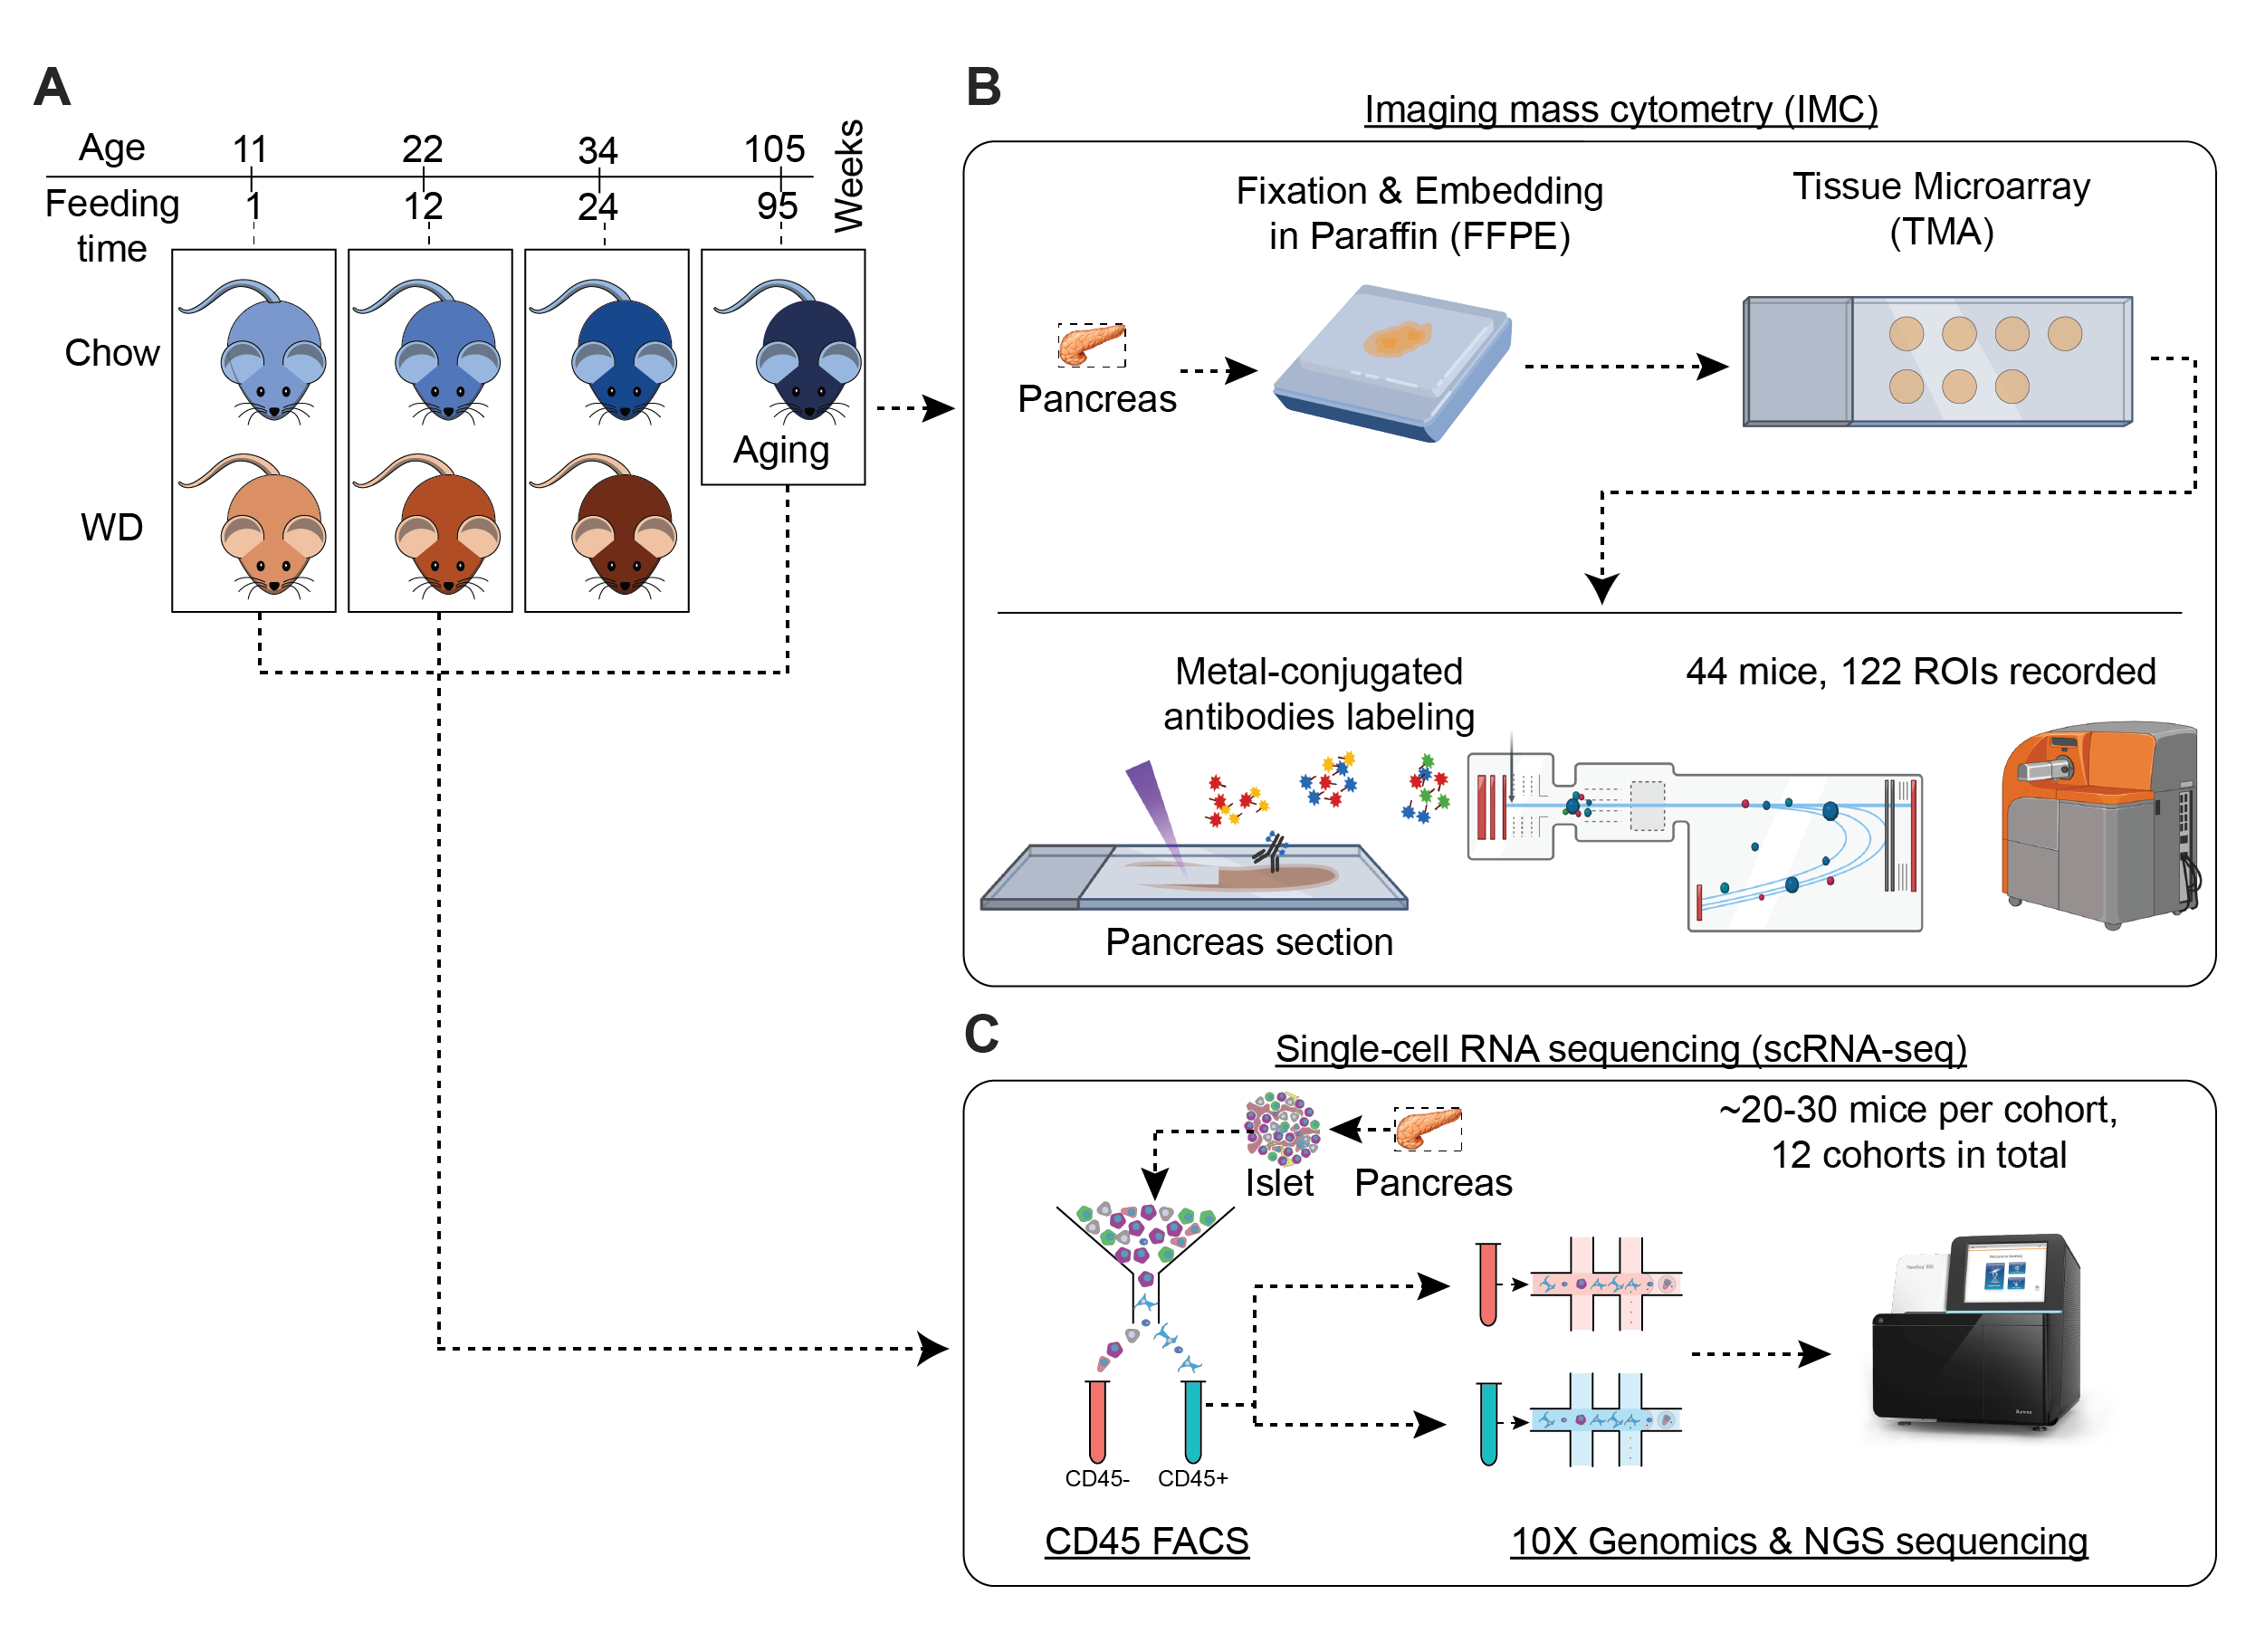
\includegraphics[width=15cm]{Chapter4/Fig/F2-1-01.png}
\caption[Experimental design to study \glsentryshort{wd}-induced obesity and aging]{\textbf{Experimental design to characterize changes in pancreatic immune cells during \gls{wd}-induced obesity and aging.} This illustration outlines the methodology where pancreas samples were harvested from at-least four mice at three post-\gls{wd} feeding time-points (W1, W12 and W24), alongside samples from age-matched, chow-fed mice and \textasciitilde2-year-old mice. These samples underwent \gls{imc} analysis using an established panel of markers targeting several immune populations, islet $\beta$-cells and endothelial cells \textbf{(\autoref{tab:app_imc_panel})}. For \gls{scr} analysis, islets from ten cohorts across early (W1) and mid-term (W12) \gls{wd} stages and two chow-fed aging cohorts, were isolated. \textasciitilde20-30 mice contributed to each cohort. Post-isolation, islet cells were \glsentryshort{facs}-sorted into immune (CD45\textsuperscript{+}) and non-immune (CD45\textsuperscript{-}) groups and processed via the 10x Genomics v3 protocol, and sequenced.}
\label{fig:chp2_experimental_design}
\end{figure}

 to \gls{wd} or a control chow diet feeding for 1 week (W1), 12 weeks (W12), or 24 weeks (W24). In addition, we incorporated samples from a cohort of \textasciitilde2-year-old to contrast between metabolic and aging-associated stress. This allowed us to compare the spatial organization of immune cells under these conditions. To complement the \gls{imc} spatial data with molecular profiles, we performed \gls{scr} on isolated CD45\textsuperscript{+} immune cells and CD45\textsuperscript{-} non-immune populations from the pancreatic islets \textbf{(}see \hyperref[subsec:met_chp2_scrdata]{\textbf{Methods}}\textbf{)}. In the \gls{scr} analysis, our objective was to detect initial molecular alterations triggered by the \gls{wd} feeding, focusing on samples collected at W1 and W12 feeding time-points \textbf{(\autoref{fig:chp2_experimental_design})}. Additionally, we also included samples from \textasciitilde2-year-old mice in order to gain further insights regarding the aging-associated inflammatory processes that trigger \gls{t2d}.  %(\textbf{Fig.\ref{fig:wdaging_experimental_design}}).


%\clearpage
\section[Unraveling complex cellular heterogeneity within the pancreatic tissue and islets]{Unraveling complex cellular heterogeneity within the\\pancreatic tissue and islets}
\label{sec:chp2_imc_scrna}

\subsubsection{\large \gls{imc} data analysis}
\label{sec_chp2_imc1}

In the \gls{imc} analysis, pancreatic tissue sections from at least 4 mice for each feeding groups and time-points were included (in total, seven experimental conditions). In total, at least 10 \glspl{roi} were sampled for each of the seven experimental conditions, and 78 \glspl{roi} were used altogether to create 17 \glspl{tma}, each containing \glspl{roi} from different experimental conditions and time-points. \glspl{tma} were then subjected to comprehensive \gls{imc} analysis of 25 selected immune cell marker proteins \textbf{(\autoref{tab:app_imc_panel};} see \hyperref[subsec:met_chp2_imcdata]{\textbf{Methods}}\textbf{)}. Additionally, we used INS, \glsentryshort{glp1}R and NKX6-1 as markers of pancreatic islets. Using a comprehensive, standardized cell segmentation workflow, we achieved single-cell resolution of our  analysis \textbf{(\autoref{fig:app_imc_segmentation};} see \hyperref[subsec:met_chp2_imcdata]{\textbf{Methods}}\textbf{)}. We also included one \gls{roi} from a spleen sample in each individual \gls{tma}. This served as a cross-\gls{tma} reference for the batch correction of immune cell marker staining intensity channels across all \glspl{tma} \textbf{(\autoref{fig:app_imc_anchorbcell} A)}.\\


\begin{figure}[t]
\centering
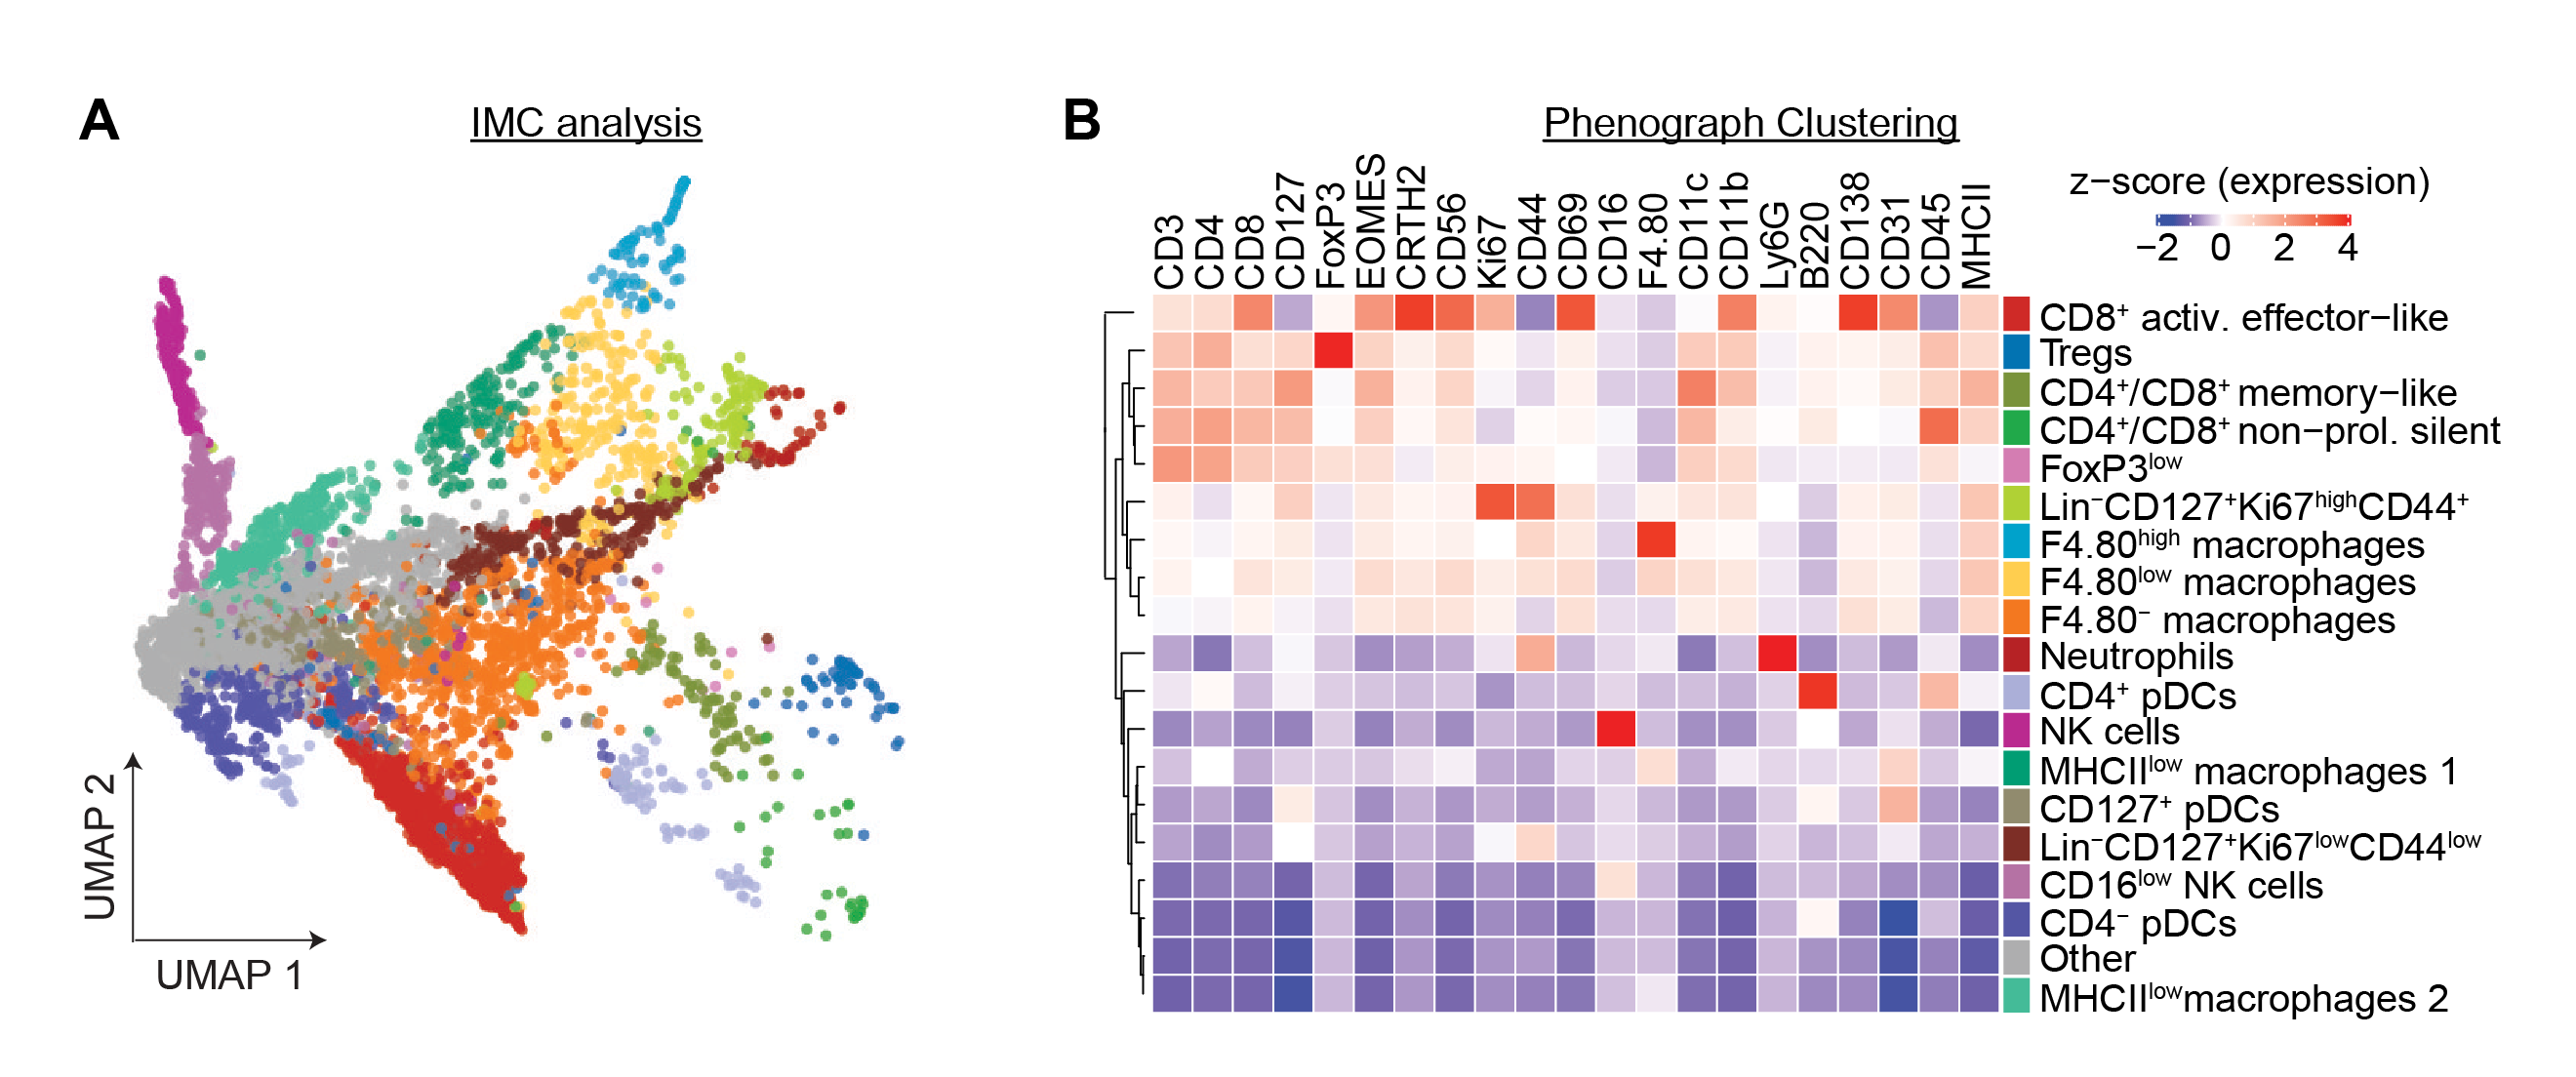
\includegraphics[width=\linewidth]{Chapter4/Fig/F2-2-01.png}
\caption[Characterization of immune cell populations with \glsentryshort{imc}]{\textbf{Characterization of immune cell populations with \gls{imc}.} \textbf{(A)} \gls{umap} embedding of the CD45\textsuperscript{+}CD19\textsuperscript{-} immune cell populations identified by \gls{imc} analysis. \textbf{(B)}  Heatmap depicting the Phenograph clustering and transformed \textit{z-scores} of protein expression for the immune cell marker channels. The identities of the sub-populations were defined based on the relative expression levels of these marker proteins. \textit{This data and figure were originally generated by Dr. Matthias Barone and reused here with permission.}}
\label{fig:chp2_imc_umap}
\end{figure}

\par The pancreatic islets were identified using the INS, NKX6-1 and \glsentryshort{glp1} channels, whereas the pancreatic lymph nodes were marked using B220, CD19, CD44 and CD45 channels \textbf{(\autoref{tab:app_imc_panel})}. Interestingly, CD19\textsuperscript{+} B-cells were nearly all localized within the pancreatic lymph nodes \textbf{(\autoref{fig:app_imc_anchorbcell} B,C)}, and were therefore not selected for subsequent analyses. Cluster analysis of the selected CD45\textsuperscript{+}CD19\textsuperscript{-} immune cells using Phenograph enabled us to identify a wide variety of immune cell populations, including different CD3 expressing T-cell sub-populations, such as EOMES\textsuperscript{+}CD56\textsuperscript{+}KI67\textsuperscript{+}CD69\textsuperscript{+} activated effector-like CD8\textsuperscript{+} cells, FOXP3\textsuperscript{+} \gls{treg}, CD127\textsuperscript{\textit{high}}CD4\textsuperscript{+}/CD8\textsuperscript{+} memory-like cells, KI67\textsuperscript{-}CD4\textsuperscript{+}/CD8\textsuperscript{+} non-proliferative silent cells, and FOXP3\textsuperscript{\textit{low}}CD4\textsuperscript{+} T-cells, differently activated macrophage sub-populations such as F4/80\textsuperscript{-}CD11c\textsuperscript{\textit{high}}, F4/80\textsuperscript{\textit{low}}CD11c\textsuperscript{\textit{high}}, F4/80\textsuperscript{\textit{high}}CD11c\textsuperscript{\textit{low}}, and two \glsentrylong{mhc2} low (\glsentryshort{mhc2}\textsuperscript{\textit{low}}) sub-populations, three types of B220 expressing plasmacytoid dendritic-like cells (\glsentryshort{pdc}) - CD4\textsuperscript{+}, CD4\textsuperscript{-}, and CD127\textsuperscript{+}, Ly6G\textsuperscript{+} neutrophils, CD16\textsuperscript{\textit{high}} natural killer (\glsentryshort{nk}) cells, and Lin\textsuperscript{-}CD127\textsuperscript{+} innate lymphoid-like cells (\glsentryshort{ilc}s) \textbf{(\autoref{fig:chp2_imc_umap})}. Thus, our \gls{imc} analysis facilitated the identification and characterization of diverse immune cell populations within the pancreatic tissue.

\subsubsection{\large \gls{scr} data analysis}
\label{sec_chp2_scrna1}
Similarly, we applied a robust \gls{qc} and data integration pipeline to our \gls{scr} data \textbf{(\autoref{fig:app_scrna_qc} A-C}, see \hyperref[subsec:met_chp2_scrdataprocess]{\textbf{Methods}}\textbf{)}, yielding 125,372 high-quality single-cell transcriptomic profiles of CD45\textsuperscript{+} immune cells and CD45\textsuperscript{-} non-immune cells, annotated based on the expression of CD45 gene, \textit{Ptprc} \textbf{(\autoref{fig:chp2_fullscRNA} A)}. The immune and the non-immune populations were further analyzed separately by assessing the respective cells, performing additional \gls{qc} steps when necessary and re-integrating the subsets to allow for more granular characterization of the immune and non-immune populations within the pancreatic islets \textbf{(}see \hyperref[subsubsec:met_chp2_immuneendo]{\textbf{Methods}}\textbf{)}.

\begin{figure}[H]
\centering
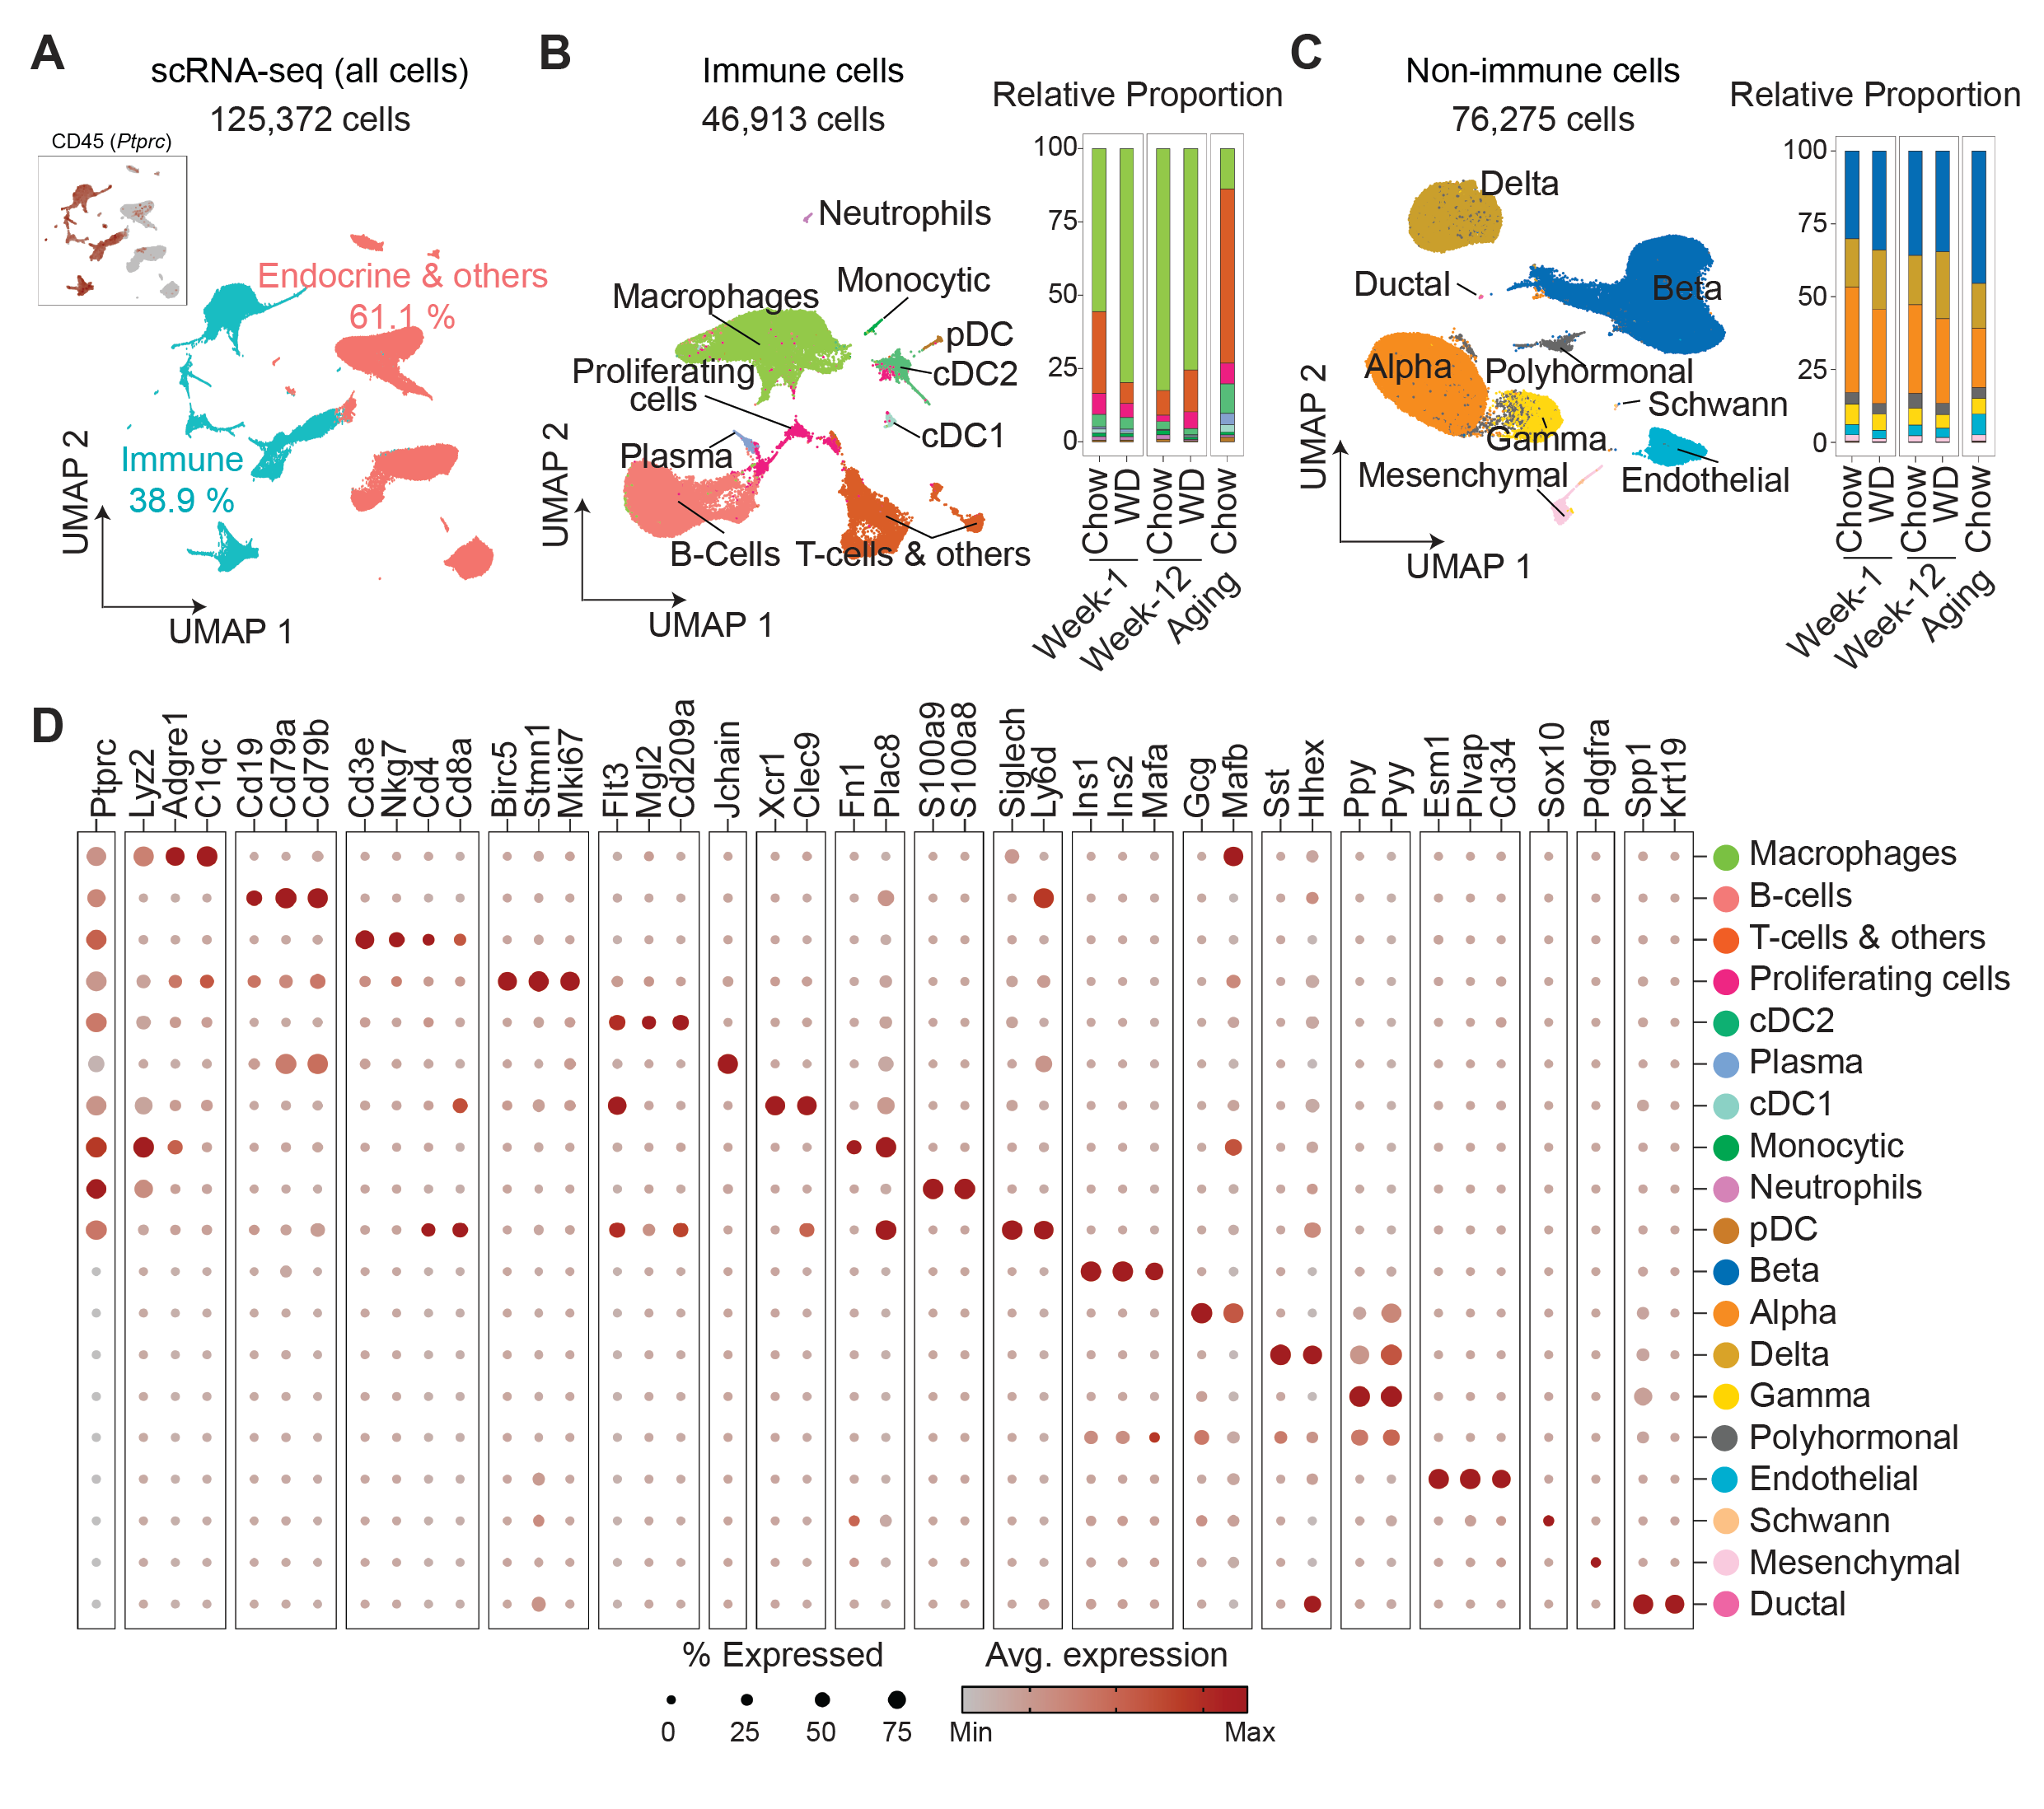
\includegraphics[width=\linewidth]{Chapter4/Fig/F2-3-01.png}
\caption[Revealing the complex heterogeneity of pancreatic islets with \glsentryshort{scr}]{\textbf{Revealing the complex heterogeneity of pancreatic islets with \gls{scr}} \textbf{(A)} \gls{umap} embedding of the integrated data consisting of 125,372 single cells across twelve cohorts. The immune cells were annotated based on the expression of CD45 (\textit{Ptprc}) and the remaining cells were labelled as `Endocrine \& others'. Values indicate the overall proportion of each annotated population. \textbf{(B)} \gls{umap} embedding of the immune cell population, following additional \gls{qc} and subsequent re-integration. Cluster identities were defined based on the expression of known immune markers. \textbf{(C)} The proportion of each annotated immune cell sub-populations computed as a percentage of total immune cells in every experimental group. The cells from different biological replicate cohorts were pooled together. B-cells were excluded from calculation and are therefore not represented. \textbf{(D)} \gls{umap} embedding of the `Endocrine \& others' cell populations, following additional \gls{qc} and subsequent re-integration. Cluster identities were defined based on the expression of known gene markers. \textbf{(E)} The proportion of each annotated endocrine, exocrine and other cell populations computed as a percentage of total non-immune cells in every experimental group. The cells from different biological replicate cohorts were pooled together. \textbf{(F)} Combined dot plot showing hallmark marker genes for all annotated cell types in \textbf{(B)} and \textbf{(D)}. The color of the dots represent the scaled average expression of the genes and the size of the dots correspond to the percentage of cells expressing the gene.}
\label{fig:chp2_fullscRNA}
\end{figure}

\par Our approach, focusing on CD45 enrichment \textbf{(\autoref{fig:chp2_experimental_design})}, allowed us to profile a total of 46,913 islet-associated immune cells, which currently represents the most comprehensive immune cell map available for mouse islets \textbf{(\autoref{fig:chp2_fullscRNA} B; \autoref{fig:app_scrna_qc} A,C)}. Utilizing the expression of known markers \textbf{(\autoref{fig:chp2_fullscRNA} F)}, we confirmed the presence of macrophages (marked by \textit{Lyz2, Adgre1, C1qc}), monocytes (identified by \textit{Fn1, Plac8}), neutrophils (\textit{S100a9, S100a8}), dendritic cells (indicated by \textit{Xcr1, Flt3, Siglech}), and a variety of lymphocytes such as T-cells (expressing \textit{Cd3e, Cd4, Cd8a}), B-cells (transcribing \textit{Cd19, Cd79a} and \textit{Cd79b}), and plasma cells (marked by \textit{Jchain}). The macrophages represented the major immune population within the islets of adult mice (W1 and W12) \textbf{(\autoref{fig:chp2_fullscRNA} C)}. However, the proportion of T-cells was highest in the cohort of older mice \textbf{(\autoref{fig:chp2_fullscRNA} C)}, which is in line with the observation of significant accumulation of T-cells in aging mice \textbf{\cite{denroche_t_2021}}. Of note, B-cells were also excluded in downstream analyses of the single-cell data, as they were primarily associated with pancreatic lymph nodes in the \gls{imc} analysis \textbf{(\autoref{fig:app_imc_anchorbcell} B,C)} and their proportion across the single-cell cohorts was also inconsistent \textbf{(\autoref{fig:app_scrna_qc} A)}. The remaining immune populations represented a minor fraction of the total islet-associated immune cells across all cohorts in the single-cell data \textbf{(\autoref{fig:chp2_fullscRNA} C)}.\\% Our \gls{scr} analysis further enabled the investigation of islet-associated immune cells at a resolution that is significantly superior to that achievable with \gls{ihc}.\\

\par We also profiled 76,275 islet-associated CD45\textsuperscript{-} cells from the same cohort of animals, which consisted of pancreatic endocrine and exocrine cells, endothelial cells, mesenchymal cells and schwann cells, based on well-established hallmark gene expression patterns \textbf{(\autoref{fig:chp2_fullscRNA} D,F; \autoref{fig:app_scrna_qc} B,C)} \textbf{\cite{van_gurp_generation_2022}}. We annotated the endocrine populations as Alpha ($\alpha$) - \textit{Gcg, Mafb}; Beta ($\beta$) -\textit{Ins1, Ins2, Mafa}; Delta ($\delta$) - \textit{Sst, Hhex} cells and Gamma ($\gamma$) - \textit{Ppy, Pyy}, also known as \gls{pp}-cells, based on the expression of primary islet hormones and \glspl{tf} \textbf{(\autoref{fig:chp2_fullscRNA} D,F)}. $\beta$-cells constituted the major fraction of endocrine cells (\textasciitilde37\%), followed by $\alpha$-cells (\textasciitilde30\%), $\delta$-cells (\textasciitilde19\%) and \gls{pp}-cells (\textasciitilde6\%) \textbf{(\autoref{fig:chp2_fullscRNA} E)}. In line with previous studies, the proportion of $\beta$-cells in the chow diet-fed aging cohort was higher compared to the all the non-aging (W1 and W12) cohorts \textbf{(\autoref{fig:chp2_fullscRNA} E)} \textbf{\cite{tuduri_pancreatic_2022}}. Consistent with methodologies employed in published reports, endocrine cells expressing more than one hormone marker were classified as polyhormonal cells and accounted for \textasciitilde4\% of the data \textbf{(\autoref{fig:app_scrna_qc} D,E)} \textbf{\cite{sachs_targeted_2020, perez-frances_pancreatic_2021}}. The other endocrine populations, as well as the exocrine cells, did not show any shifts in their cellular proportions in response to metabolic stress or aging. The mesenchymal (2\%), schwann (1\%), ductal (1\%) and endothelial (5\%) cells together made up less that 10\% of the single-cell data \textbf{(\autoref{fig:chp2_fullscRNA} E)}, thereby reflecting the efficiency of the islet isolation step during sample preparation.\\

\par Thus, the CD45\textsuperscript{+} enrichment combined with single-cell transcriptomics enabled a detailed characterization of the immune landscape within pancreatic islets. Further, integrating with \gls{imc}, we have constructed a comprehensive representation of the immune cells within the mouse pancreas, encompassing both their spatial distribution and molecular characteristics. 

%\clearpage

\section[Metabolic stress accelerates aging-induced accumulation of inflammatory F4/80\textsuperscript{\textit{low}} macrophages]{Metabolic stress accelerates aging-induced accumulation \\of inflammatory F4/80\textsuperscript{\textit{low}} macrophages}
\label{sec:imc_acceleration}

We subsequently investigated whether immune cell populations within the pancreas expanded in response to \gls{wd}-feeding or aging. Using \gls{imc}, we assessed the density of each immune cell population and detected significant changes in the macrophage abundance across metabolic stress and aging \textbf{(\autoref{tab:app_imc_macrophages})}. This affected the three macrophage sub-populations expressing various levels of CD11c and F4/80: F4/80\textsuperscript{\textit{high}}, F4/80\textsuperscript{\textit{low}}, and F4/80\textsuperscript{\textit{-}} \textbf{(\autoref{fig:chp2_imc_umap} B, \autoref{fig:chp2_imc_macrophages1} A)}. Our analysis primarily centered on two major aspects of sub-population dynamics: 
\begin{enumerate}
    \item The relative enrichment of these cells within the entire pancreas and
    \item The accumulation of these immune cells in specific regions, namely the pancreatic islets and the peri-islet areas.
\end{enumerate}

To address the second aspect, we identified the islet regions based on INS, NKX6-1 and \glsentryshort{glp1} channels. To evaluate both, the expansion of islet-resident immune cells and the recruitment of immune cells to the periphery of the islet, we defined a peri-islet region that extended 70\textmu m beyond the boundary of the identified islets \textbf{(\autoref{fig:chp2_imc_macrophages1} B)}. Our --


\begin{figure}[H]
    \centering
    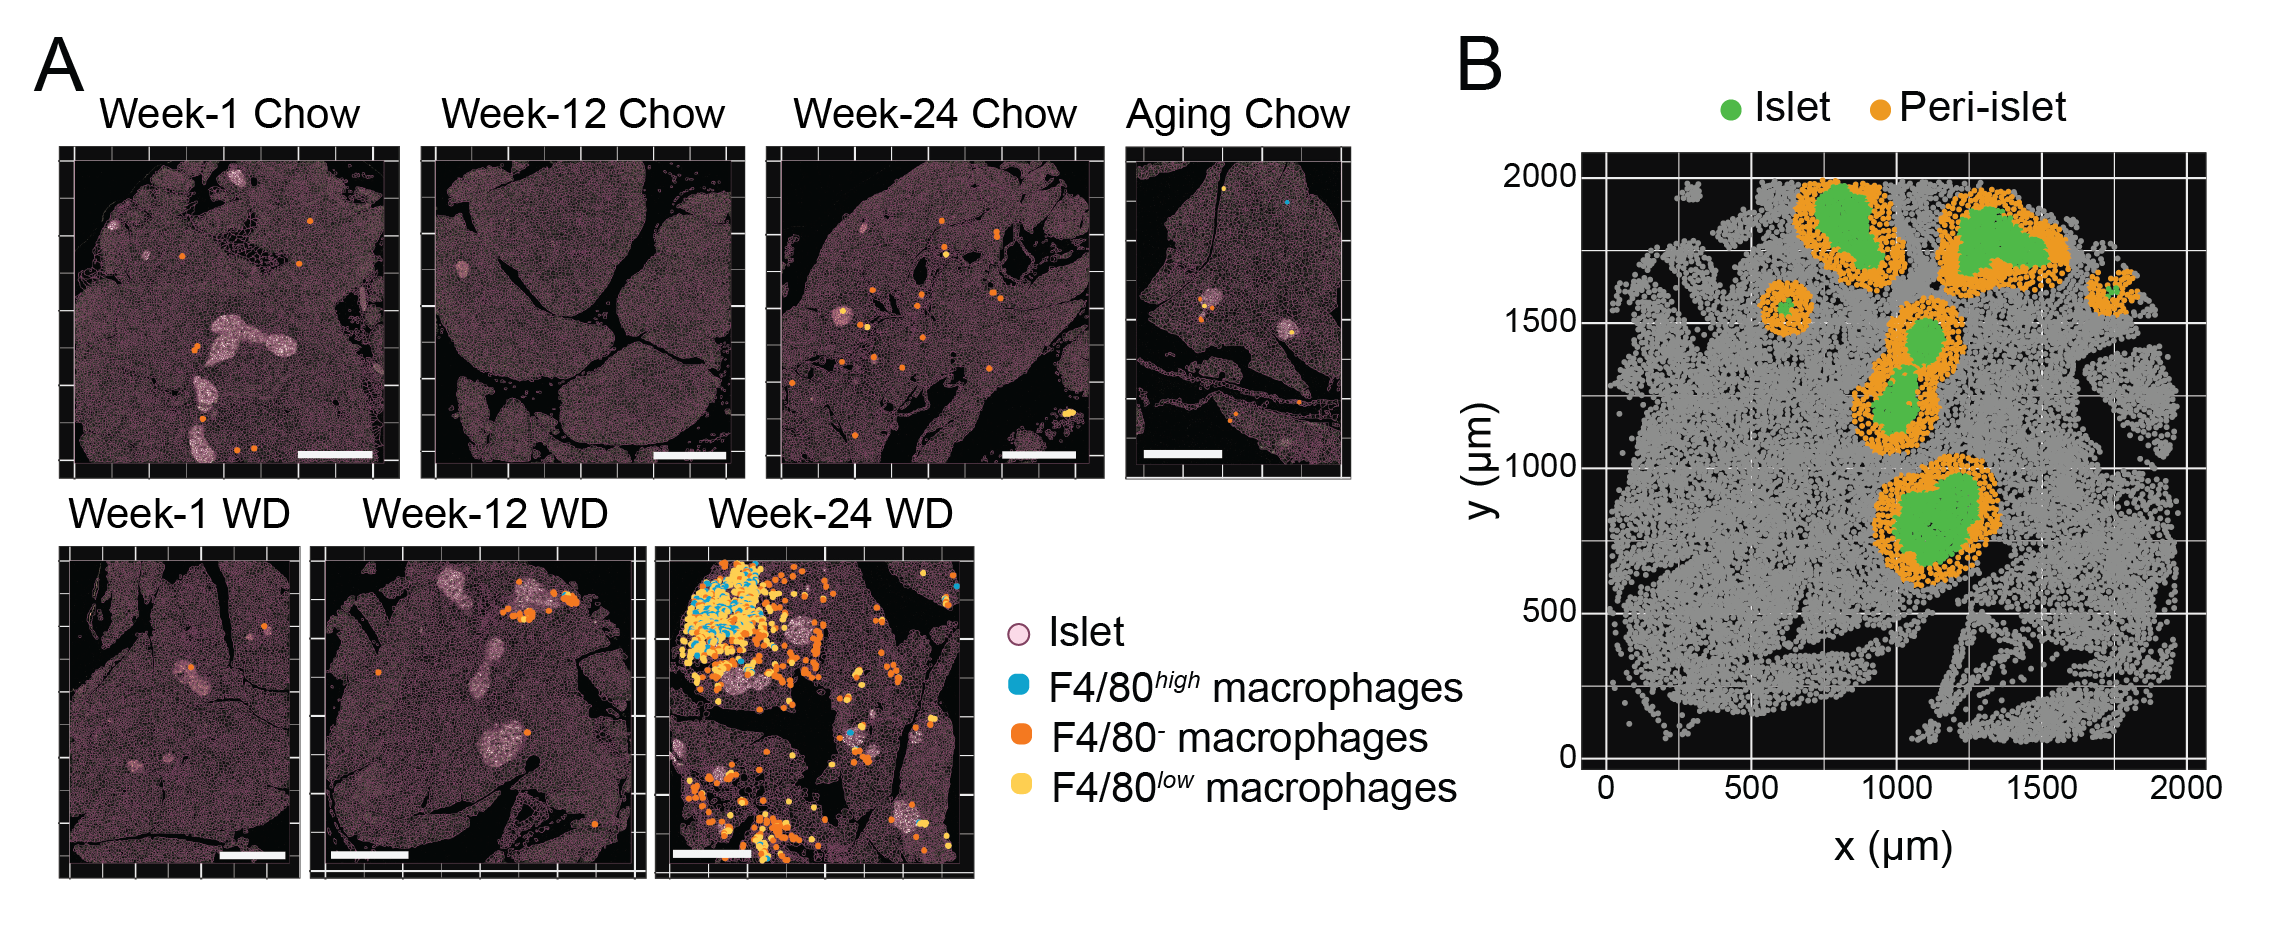
\includegraphics[width=\linewidth]{Chapter4/Fig/F2-9-01.png}
    \caption[Mapping macrophages within pancreatic tissue]{\textbf{Mapping macrophages within pancreatic tissue.} \textbf{(A)} Representative \glspl{roi} showing the three macrophage sub-populations expressing different levels of CD11c and F4/80: F4/80\textsuperscript{\textit{high}}, F4/80\textsuperscript{\textit{low}}, and F4/80\textsuperscript{\textit{-}} in the pancreas. Pancreatic islet regions are marked by INS channel. Scale bar 500 \textmu m. \textbf{(B)} Representative image illustrating a pancreatic islet (green) enclosed by peri-islet region (yellow) encompassing the area extending from the islet boundary up to 70\textmu m away. \textit{This data and figure were originally generated by Dr. Matthias Barone and reused here with permission.}}
    \label{fig:chp2_imc_macrophages1}
\end{figure}
 
-- observations indicated that most immune cell populations in the pancreas remained stable under metabolic stress or progressive aging \textbf{(\autoref{fig:chp2_imc_macrophages2} A, \autoref{fig:app_imc_macrophages})}. However, there was a notable increase in F4/80\textsuperscript{\textit{low}} macrophages across the entire pancreas \textbf{(\autoref{fig:chp2_imc_macrophages2} A}, middle\textbf{; \autoref{fig:app_imc_macrophages} B,E)}. These cells also accumulated within the islets and their adjacent areas. Due to the higher variability in \gls{wd} feeding, this became only significant in the aging condition \textbf{(\autoref{fig:chp2_imc_macrophages2} B}, middle\textbf{)}. Overnutrition also caused a mild elevation in F4/80\textsuperscript{\textit{-}} macrophages throughout the pancreas \textbf{(\autoref{fig:chp2_imc_macrophages2} A}, right\textbf{; \autoref{fig:app_imc_macrophages} C,F)}, whereas F4/80\textsuperscript{\textit{high}} macrophages stayed constant, irrespective of the conditions \textbf{(\autoref{fig:chp2_imc_macrophages2} A}, left\textbf{; \autoref{fig:app_imc_macrophages} A,D)}. Additionally, neither F4/80\textsuperscript{\textit{high}} \textbf{(\autoref{fig:chp2_imc_macrophages2} B}, left\textbf{)}  and F4/80\textsuperscript{\textit{-}} \textbf{(\autoref{fig:chp2_imc_macrophages2} B}, right\textbf{)} macrophages moved closer to the islet region under either of the metabolic stresses.\\

\begin{SCfigure}[][h]
  \centering
  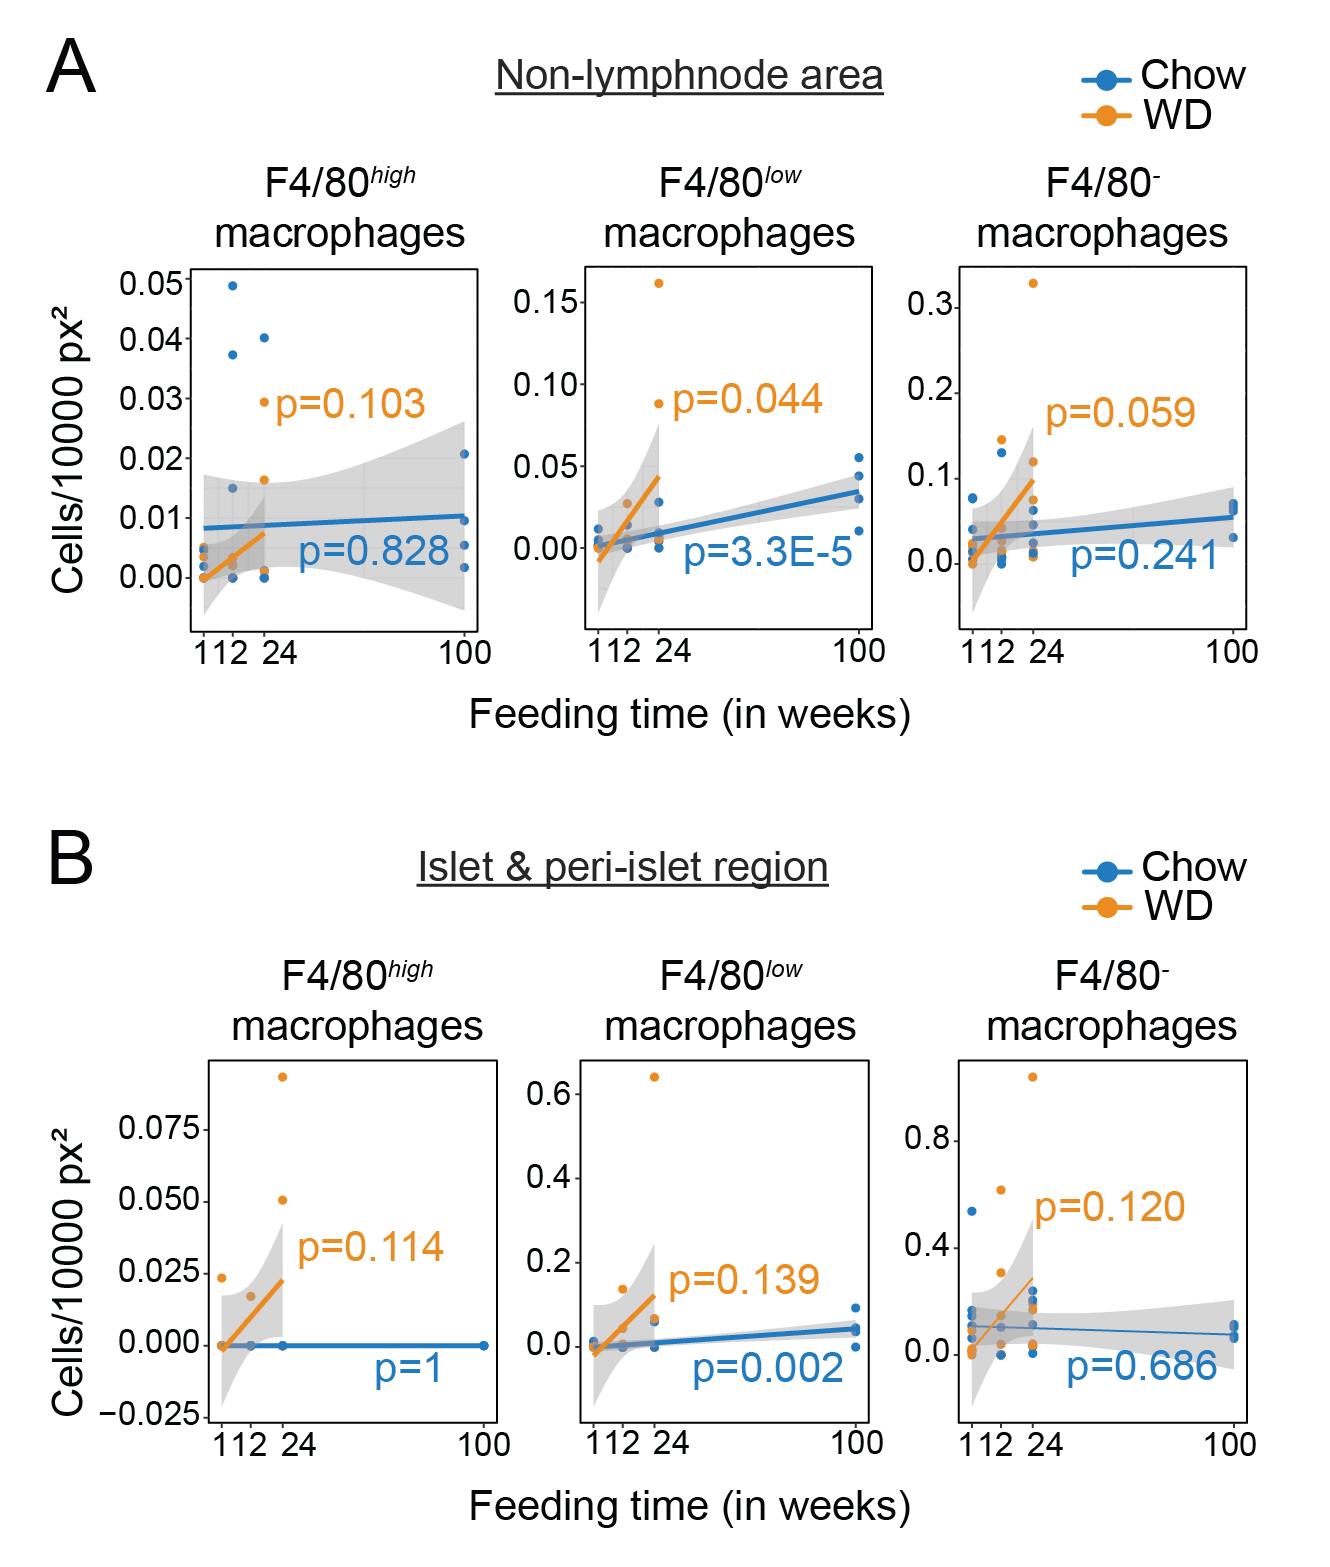
\includegraphics[width=0.5\linewidth]{Chapter4/Fig/F2-9-02.png}
  \vspace{-10pt}
  \caption[Accumulation of inflammatory macrophages within the pancreas]{\textbf{\gls{wd} accelerates aging-induced accumulation of inflammatory F4/80\textsuperscript{\textit{low}} macrophages}.\textbf{(A) - (B)} Scatter plots depicting the cell counts of F4/80\textsuperscript{\textit{high}}, F4/80\textsuperscript{\textit{low}} and F4/80\textsuperscript{\textit{-}} macrophages per area of the pancreas (excluding lymph nodes) \textbf{(A)} and per area within the pancreatic islets and peri-islet regions \textbf{(B)}  across all experimental conditions. Linear regression fits representing the cell count per area trends over time are plotted as solid lines. The 95\% confidence intervals for each linear regression are highlighted in grey. p-values for regressions were determined using t-tests. \textit{This data and figure were originally generated by Dr. Matthias Barone and reused here with permission.}}
  \label{fig:chp2_imc_macrophages2}

\end{SCfigure}

\vspace{20pt}

\par In summary, our analysis revealed a \gls{wd} feeding accelerated the accumulation of F4/80\textsuperscript{\textit{low}} macrophages within the pancreas, an effect that occurs naturally during aging under chow diet. Interestingly, conditions of overnutrition also promote the accumulation of another inflammatory macrophage sub-population - F4/80\textsuperscript{-} macrophages, which did not increase with aging.%  -mediated acceleration of the accumulation of the F4/80\textsuperscript{\textit{low}} macrophages within the pancreas and peri-islet regions, which under chow diet only happens later in life. Metabolic stress also favored accumulation of another inflammatory CD11c\textsuperscript{\textit{high}} expressing F4/80\textsuperscript{\textit{-}} macrophages, which was not observed in aging.

% \begin{figure}
% \floatbox[{\capbeside\thisfloatsetup{capbesideposition={right,top},capbesidewidth=4cm}}]{figure}[\FBwidth]
% {\caption{A test figure with its caption side by side}\label{fig:test}}
% {\includegraphics[width=5cm]{}}
% \end{figure}

% \begin{figure}
%     \floatbox[{\capbeside\thisfloatsetup{capbesideposition={right,top},capbesidewidth=4cm}}]{figure}[\FBwidth]
    
%     {\caption{Caption}\label{fig:enter-label}}
%     {\includegraphics{}}
    
% \end{figure}


% \mysidecaption{0.4}{%
% \captionof{figure}[Linking macrophage sub-populations between scRNA-seq and IMC analyses]{\textbf{.} \textbf{(A)} Violin plots depicting the normalized expression levels of selected markers with corresponding channels in the IMC panel. The top plots compare these levels across various macrophage sub-populations, and the bottom plots display their expression in the Macs-3 population under different experimental conditions. \textbf{(B)}Heatmap showing z-scored expression of selected IMC channgels across the four macrophage sub-populations identified in the IMC analysis. Corresponding macrophage sub-populations from scRNA-seq analysis are indicated in parantheses. \textbf{(C)} Violin plots of \textit{arcsinh} transformed expression of selected IMC channels in the F4/80\textsuperscript{\textit{low}} macrophage sub-population from the IMC analysis across experimental conditions. * p<0.05, ** p<0.01, *** p<0.001 and **** p<0.0001. p-values were calculated using the Wilcoxon rank-sum test with Bonferroni correction.}%
% }
% {%
% \begin{figure}
%    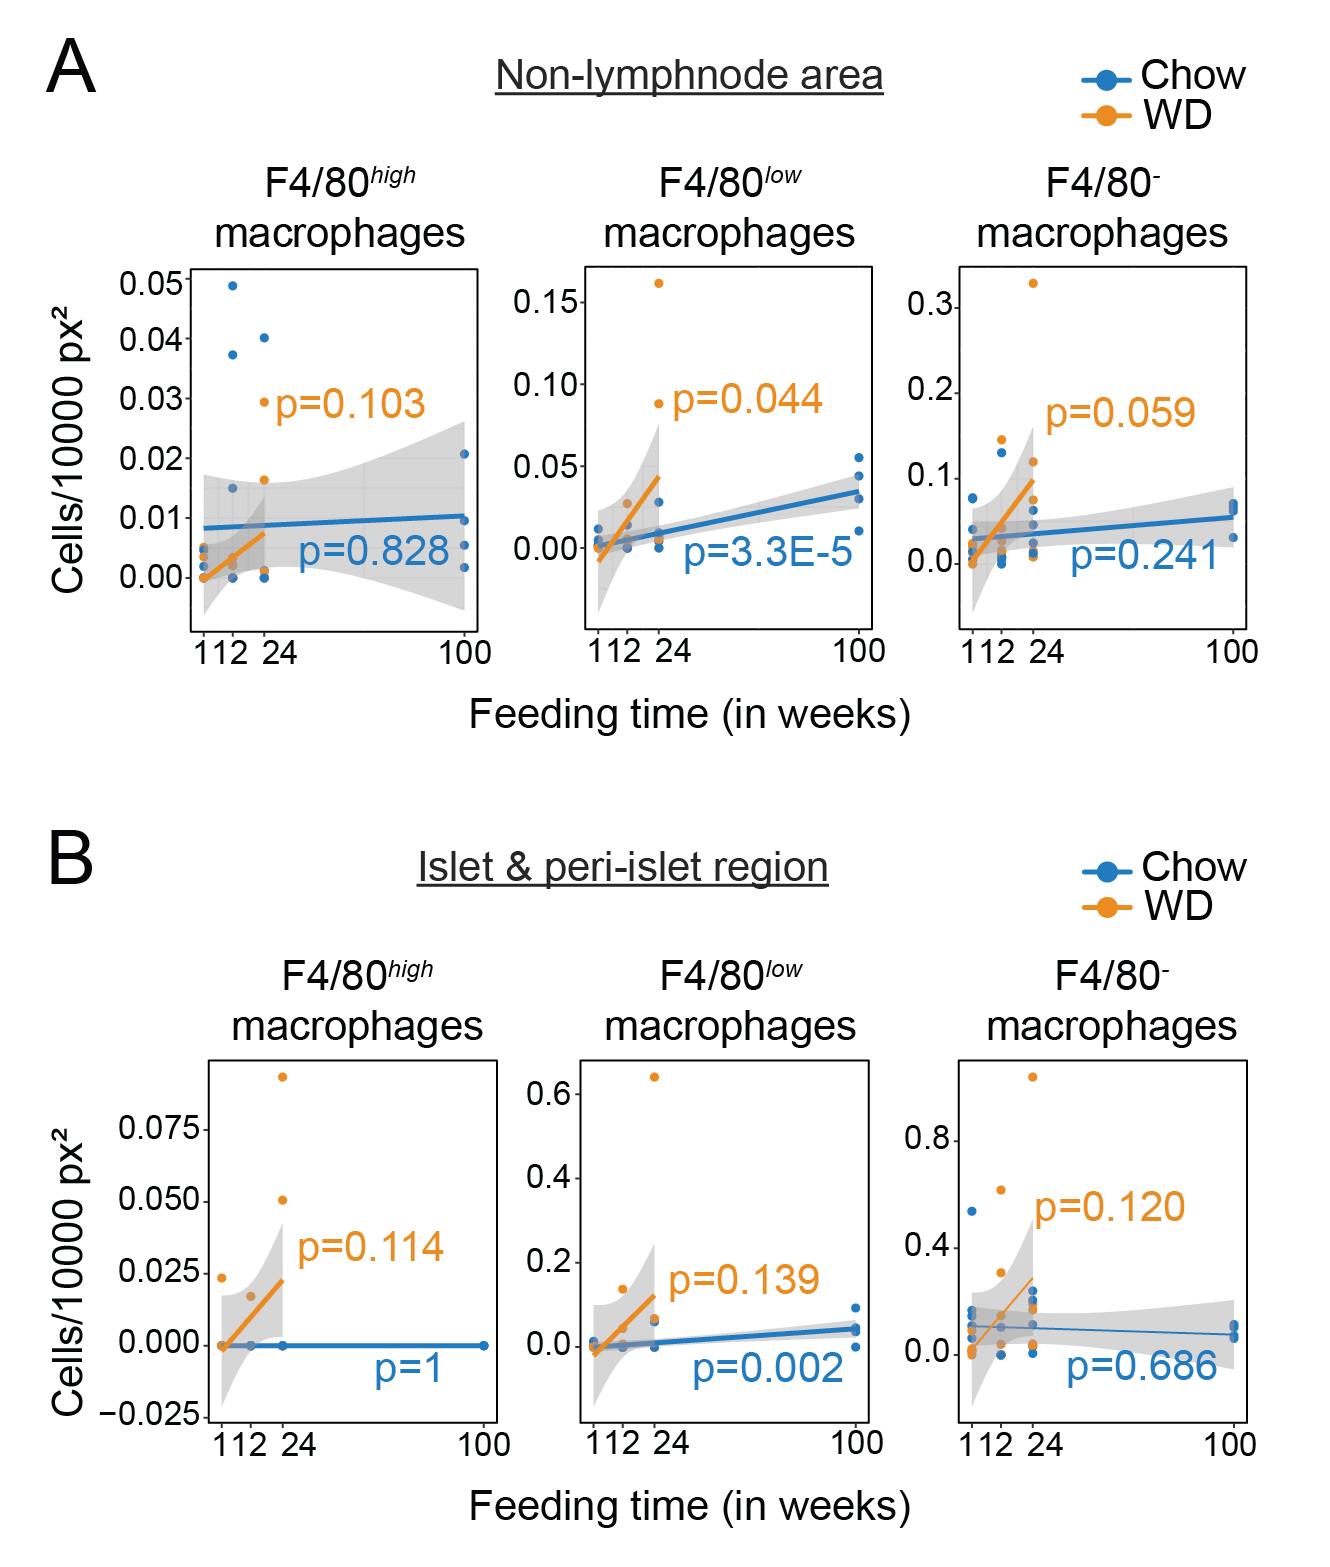
\includegraphics[width=9cm,height=11cm,keepaspectratio]{Chapter4/Fig/F2-9-02.png}%
%    \label{fig:chp2_imc_macrophages2}
% \end{figure}
% }[t]%



% \begin{figure}[b]
%     \centering
%     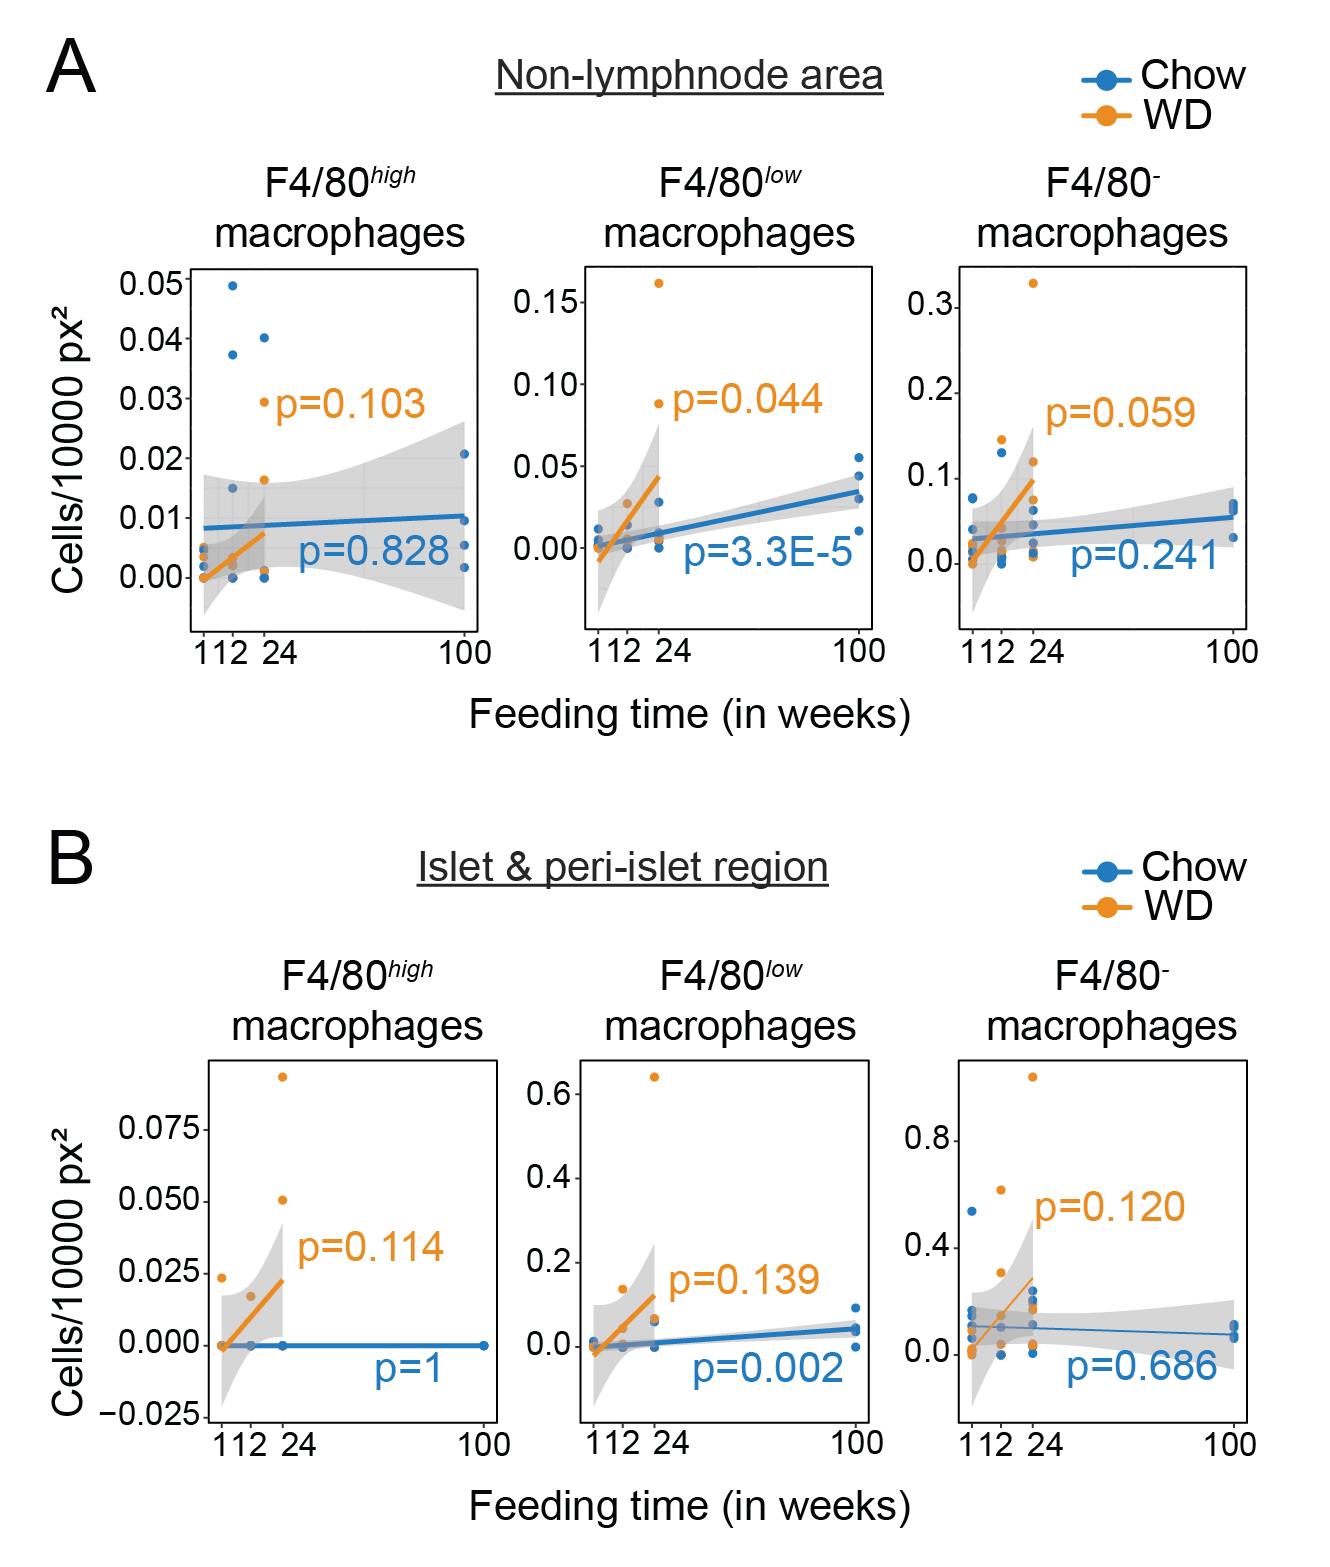
\includegraphics[width=\linewidth]{Chapter4/Fig/F2-9-02.png}
%     \caption[Accumulation of inflammatory macrophages within the pancreas]{\textbf{\gls{wd} accelerates aging-induced accumulation of inflammatory F4/80\textsuperscript{\textit{low}} macrophages.} \textbf{(A) - (B)} Scatter plots showing the cell counts of F4/80\textsuperscript{\textit{high}}, F4/80\textsuperscript{\textit{low}} and F4/80\textsuperscript{\textit{-}} macrophages per area of the pancreas (excluding lymph nodes) \textbf{(A)} and per area within the pancreatic islets and peri-islet regions \textbf{(B)}  across four time-points and two feeding conditions. Linear regression fits representing the cell count per area trends over time are plotted as solid lines. The 95\% confidence intervals for each linear regression are highlighted in grey. p-values for regressions were determined using t-tests. \textit{This data and figure were originally generated by Dr. Matthias Barone and reused here with permission.}}
%     \label{fig:chp2_imc_macrophages2}
% \end{figure}


\clearpage

\section[\glsentryshort{ifn}-activated macrophages are enriched in the islets in response to metabolic- and aging-induced stress]{Interferon-activated macrophages are enriched in the\\islets in response to metabolic- and aging-induced stress}
\label{sec:chp2_sc_macs}

% %\subsection{Characterization of islet-intrinsic macrophage sub-populations\\using scRNA-seq\\}
% Macrophages are the only resident myeloid cells found in islets of all mouse strains, under normal conditions \textbf{\cite{zakharov_single-cell_2020}}. The presence of islet-resident macrophages is essential for the normal islet development, $\beta$-cell regeneration and regulation of insulin secretion \textbf{\cite{ying_expansion_2019}}. In diet-induced islet inflammation, islet-resident macrophages have been shown to impair $\beta$-cell insulin secretion while also promoting adaptive $\beta$-cell proliferation % via PDGFR signaling. This suggests that macrophages within islets are heterogeneous in function and that diet could alter the abundance of specific macrophage subsets in pancreatic islets.

While the role of islet macrophages in perpetuating islet inflammation is known, discrepancies exists around nature of islet macrophages in insulin-resistant and \gls{t2d} models. We therefore performed detailed single-cell characterization of the islet-associated macrophages identified in our \gls{scr} data. 

\subsubsection{\large Annotating islet-intrinsic macrophages using gene expression}
 
\par To characterize the islet-associated macrophages, we extracted the macrophages from the CD45\textsuperscript{+} immmune single-cell dataset and performed sub-clustering analysis \textbf{(}see \hyperref[subsubsec:met_chp2_immuneendo]{\textbf{Methods}}\textbf{)}. We identified a total of five macrophage sub-populations which included a homeostatic, non-activated population (Macs-1), two activated populations, (Macs-2 and Macs-3), a proliferating population (Macs-4), and a phagocytic population (Macs-5) \textbf{(\autoref{fig:chp2_scrna_macrophages} A)}. Contrary to the homeostatic Macs-1, both Macs-2 and Macs-3 displayed a pro-inflammatory phenotype, characterized by type-2 and type-1 \gls{ifn} response gene signature respectively. The level of activation was more dramatic in Macs-3 than in Macs-2 \textbf{(\autoref{fig:chp2_scrna_macrophages} B,C; \autoref{tab:app_scrna_macrophages_markers})}. Intriguingly, the highest expression of \textit{Ifnb1} was observed in Macs-2, suggesting it as the likely initiator of the \gls{ifn} response \textbf{(\autoref{fig:app_scrna_macrophages_macs2_genes} A)}. Additionally, Macs-2 showed higher expression of genes downstream of \gls{tnf} and \gls{nfkb} when compared to Macs-1, a trait that was not present in Macs-3 \textbf{(\autoref{fig:chp2_scrna_macrophages} C)}. Macs-4 represented group of islet-macrophages expressing genes involved in cell-cycle pathways, and together with Macs-1, likely constitute the macrophages involved in islet homeostatic functions \textbf{(\autoref{fig:chp2_scrna_macrophages} B,C; \autoref{tab:app_scrna_macrophages_markers})}. This finding of islet macrophages with self-replicating capacity is consistent with a previous study \textbf{\cite{calderon_pancreas_2015}}. Finally, the gene expression signature of Macs-5 was associated with apoptotic cell clearance and strong anti-inflammatory function marked by the expression of \textit{Prdx1} and \textit{Lgals3} \textbf{(\autoref{fig:chp2_scrna_macrophages} B,C; \autoref{tab:app_scrna_macrophages_markers})}.\\

\begin{figure}[t!]
\centering
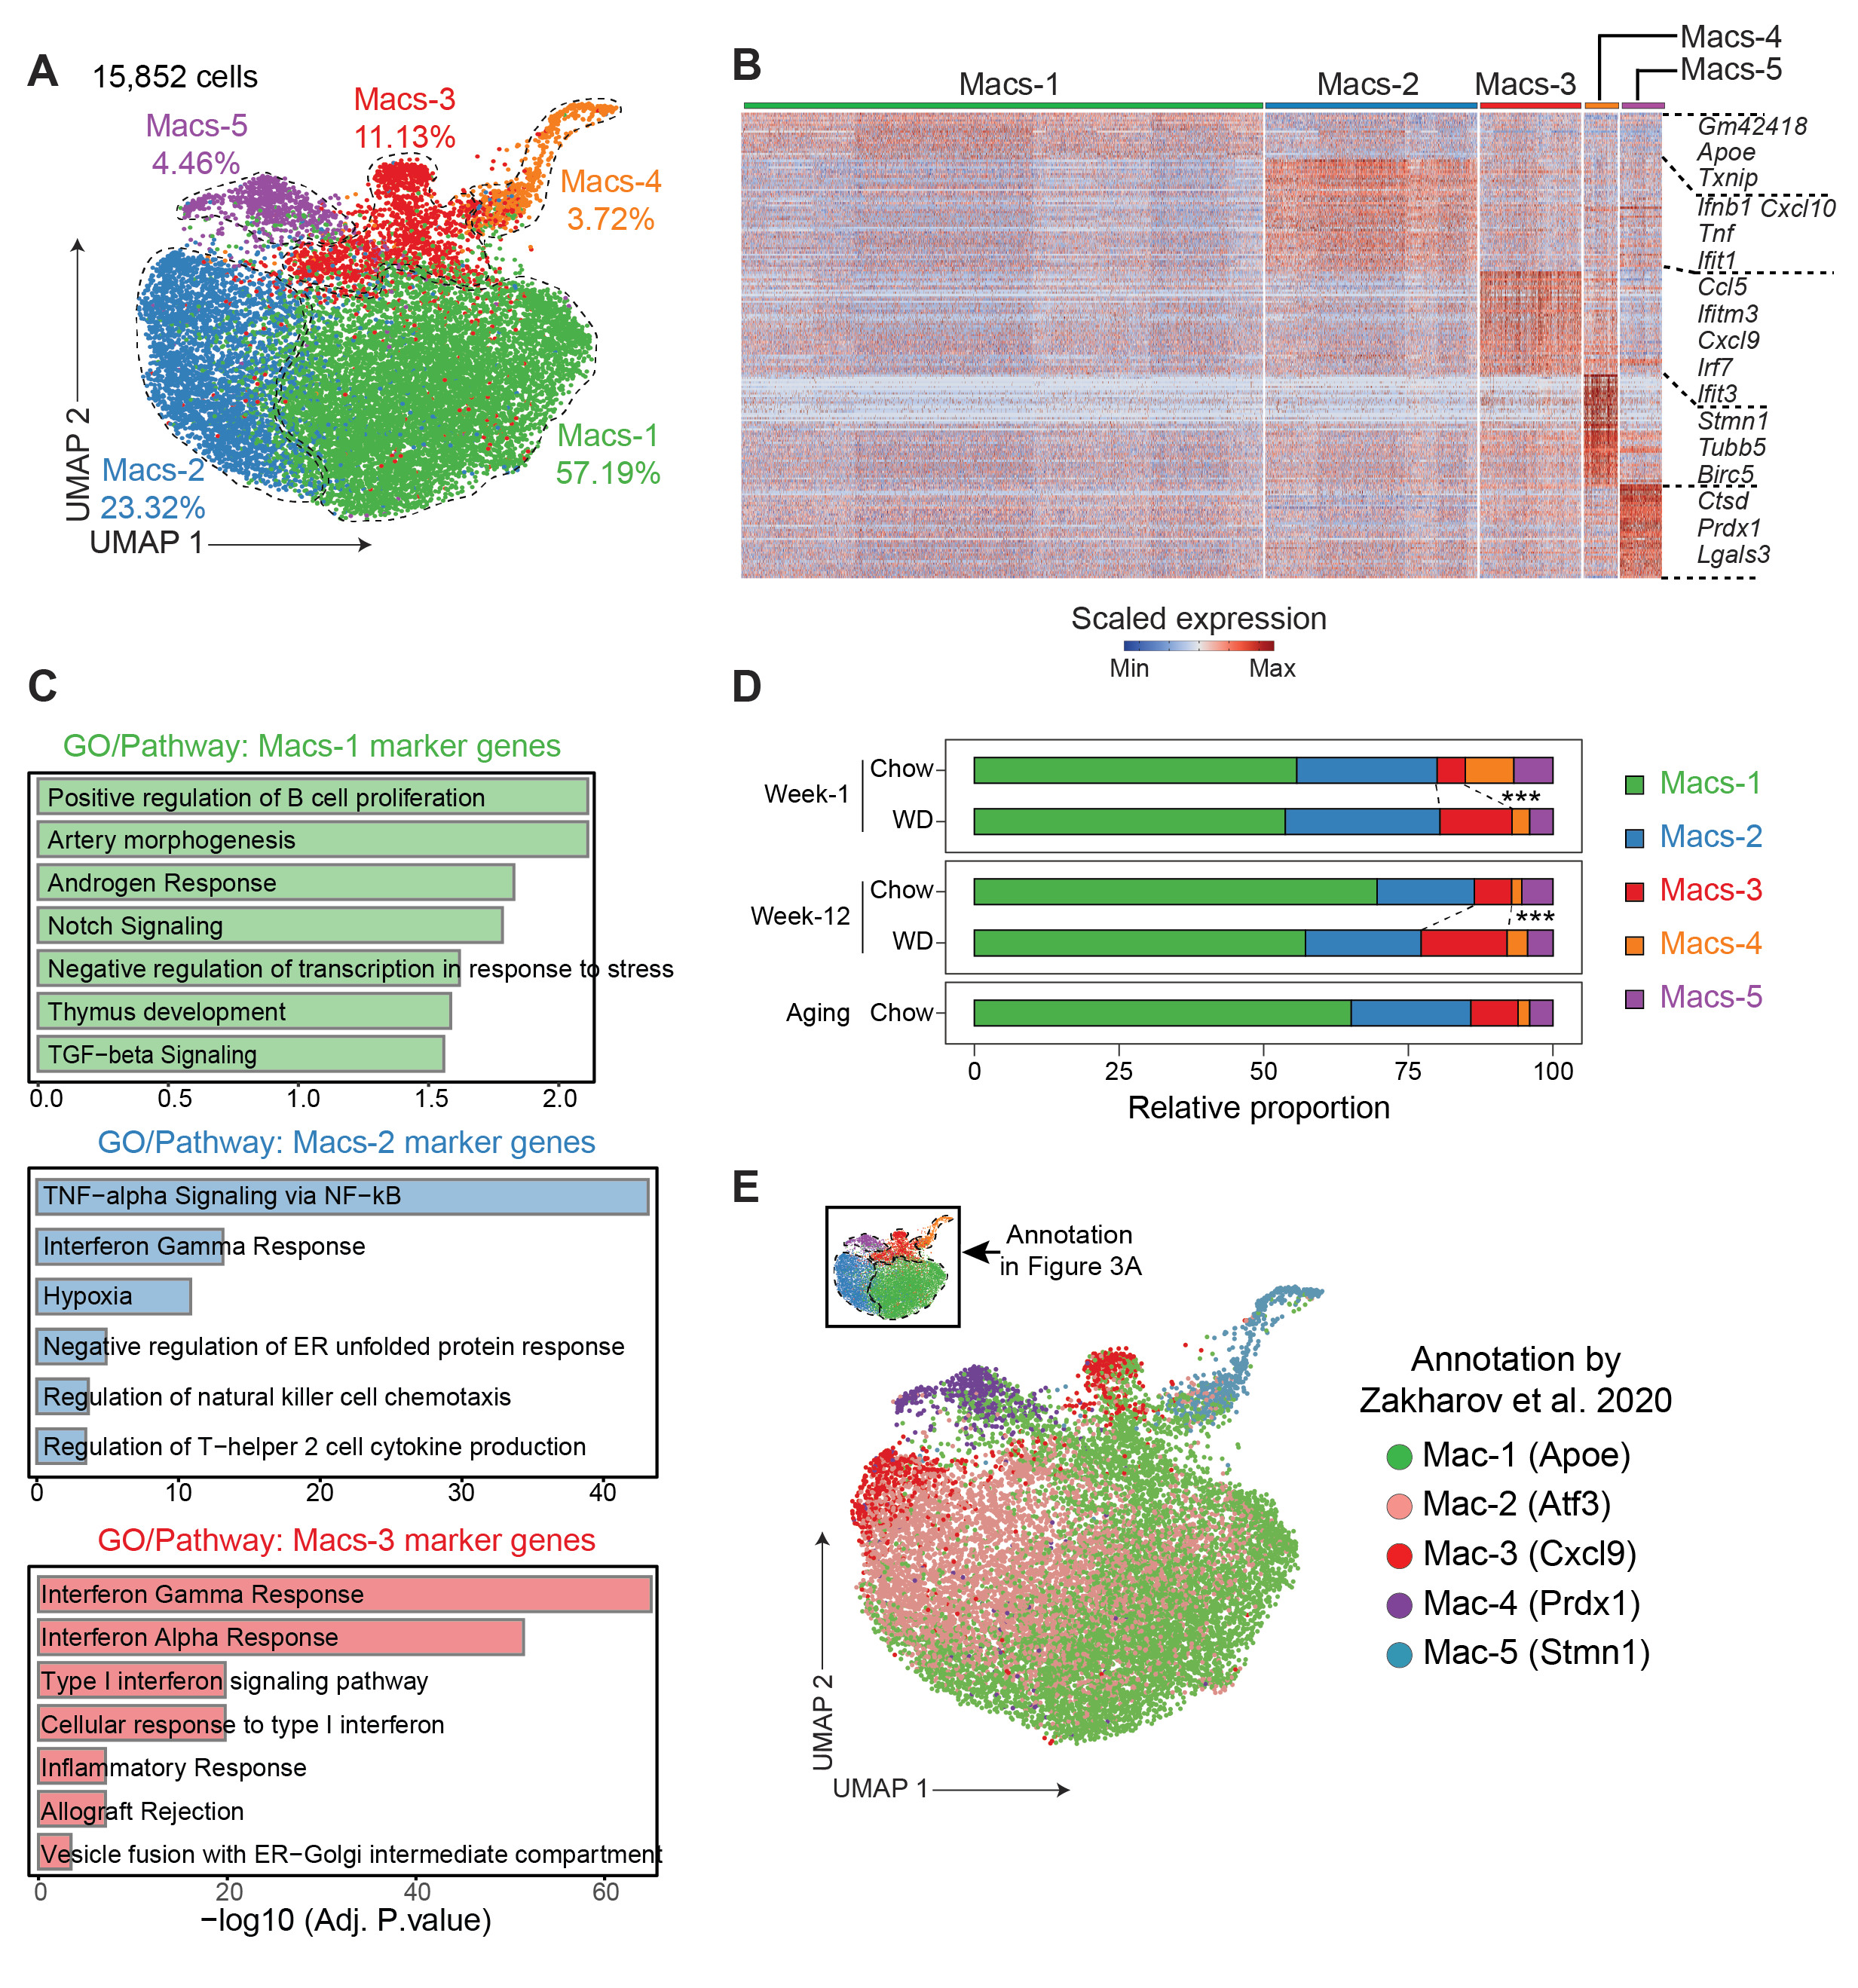
\includegraphics[width=\linewidth]{Chapter4/Fig/F2-5-01.png}
\caption[Characterization of islet-intrinsic macrophages using \glsentryshort{scr}]{\textbf{Characterization of islet-intrinsic macrophages using \gls{scr}}. \textbf{(A)} \gls{umap} embedding of pancreatic islet associated macrophages, pooled across three time-points (W1, W12 and Aging) and two dietary conditions (Chow and \gls{wd}). Values indicate the overall proportion of each defined sub-population. The identities of sub-populations were defined based on marker gene expression. \textbf{(B)} Heatmaps showing scaled expression levels of marker genes in each macrophage sub-population. \textbf{(C)} Enriched \gls{go} terms using top markers for the five macrophage sub-populations. Significance ($-\log_{10}$ adjusted p-value) of the enrichment are shown in bar plots. \textbf{(D)} The proportion of each macrophage sub-population in \textbf{(A)}, computed as a percentage of total macrophage cell numbers in every experimental group. The cells from different biological replicate cohorts were pooled together. $\textsuperscript{*} p < 0.05, \textsuperscript{**} p < 0.01, \textsuperscript{***} p < 0.001$. p-values were calculated from a mixed-effects binomial model. }
\label{fig:chp2_scrna_macrophages}
\end{figure}

% \begin{wrapfigure}{r}{0.5\textwidth}
% \vspace{-20pt} 
% 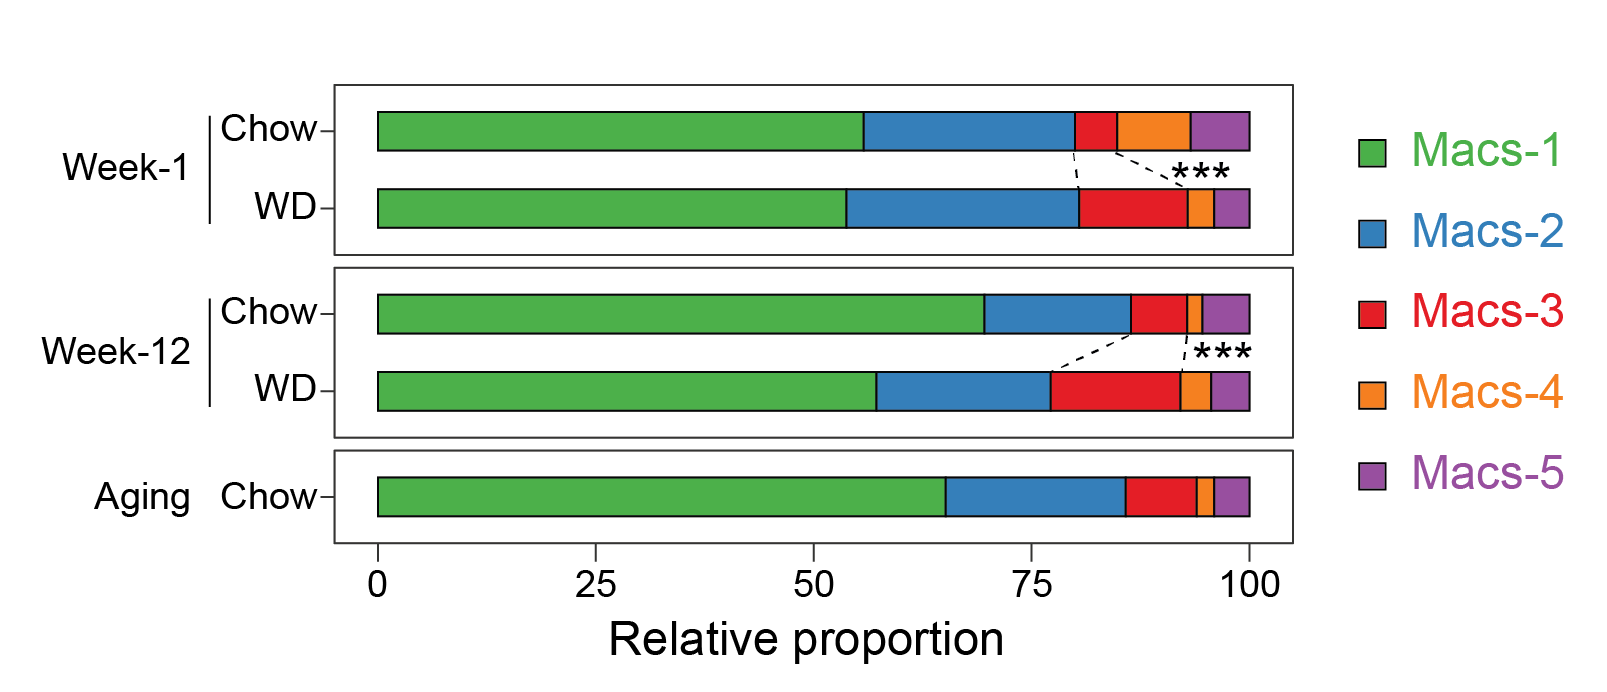
\includegraphics[width=7.5cm]{Chapter4/Fig/F2-5-03.png}
% \caption[Proportions of islet-intrinsic macrophages]{\textbf{Relative proportions of islet macrophages across \gls{wd}-feeding and aging}. Proportion of each macrophage sub-population in \textbf{(\autoref{fig:chp2_scrna_macrophages} A)}, computed as a percentage of total macrophage cell numbers in every experimental group. The cells from different biological replicate cohorts were pooled together. *: p<0.05, **: p<0.01, ***: p<0.001. p-values were calculated from a mixed-effects binomial model.}
% \label{fig:chp2_scrna_macrophages_composition}
% \vspace{-10pt}
% \end{wrapfigure} This increase could be likely to further support islet homeostasis as the mice age. 

\par The proportion of the non-inflammatory Macs-1 was the highest among all islet macrophage sub-populations, with over 50\% of the cells identified as Macs-1 in all conditions \textbf{(\autoref{fig:chp2_scrna_macrophages} D)}. Intriguingly, the W12-Chow and the Aging-Chow groups exhibited a notable higher proportion of the homeostatic Macs-1 macrophages compared to their W1-Chow counterparts \textbf{(\autoref{fig:chp2_scrna_macrophages} D)}. There was a rapid and significant expansion of the Macs-3 macrophages in response to \gls{wd} feeding, and a comparable, albeit less obvious increase during aging \textbf{(\autoref{fig:chp2_scrna_macrophages} D)}. This mirrors the stress-induced accumulation of F4/80\textsuperscript{\textit{low}} macrophages not just in the pancreas, but also in the islets and the peri-islet region \textbf{(\autoref{fig:chp2_imc_macrophages2} A}, middle\textbf{; \autoref{fig:chp2_imc_macrophages2} B}, middle\textbf{)}. In addition to these shifts, while there was a marked decrease in the proportion of the proliferating Macs-4 macrophages in response to short-term \gls{wd} feeding for 1 week, the pro-inflammatory Macs-2 and the phagocytotic Macs-5 macrophages were relatively stable during the course of \gls{wd}-feeding and aging \textbf{(\autoref{fig:chp2_scrna_macrophages} D)}.

%\clearpage

\subsubsection{\large Mapping islet-macrophages from \glsentryshort{nod} mouse model of \glsentryshort{t1d}}

% \begin{wrapfigure}{l}{0.5\textwidth}
% 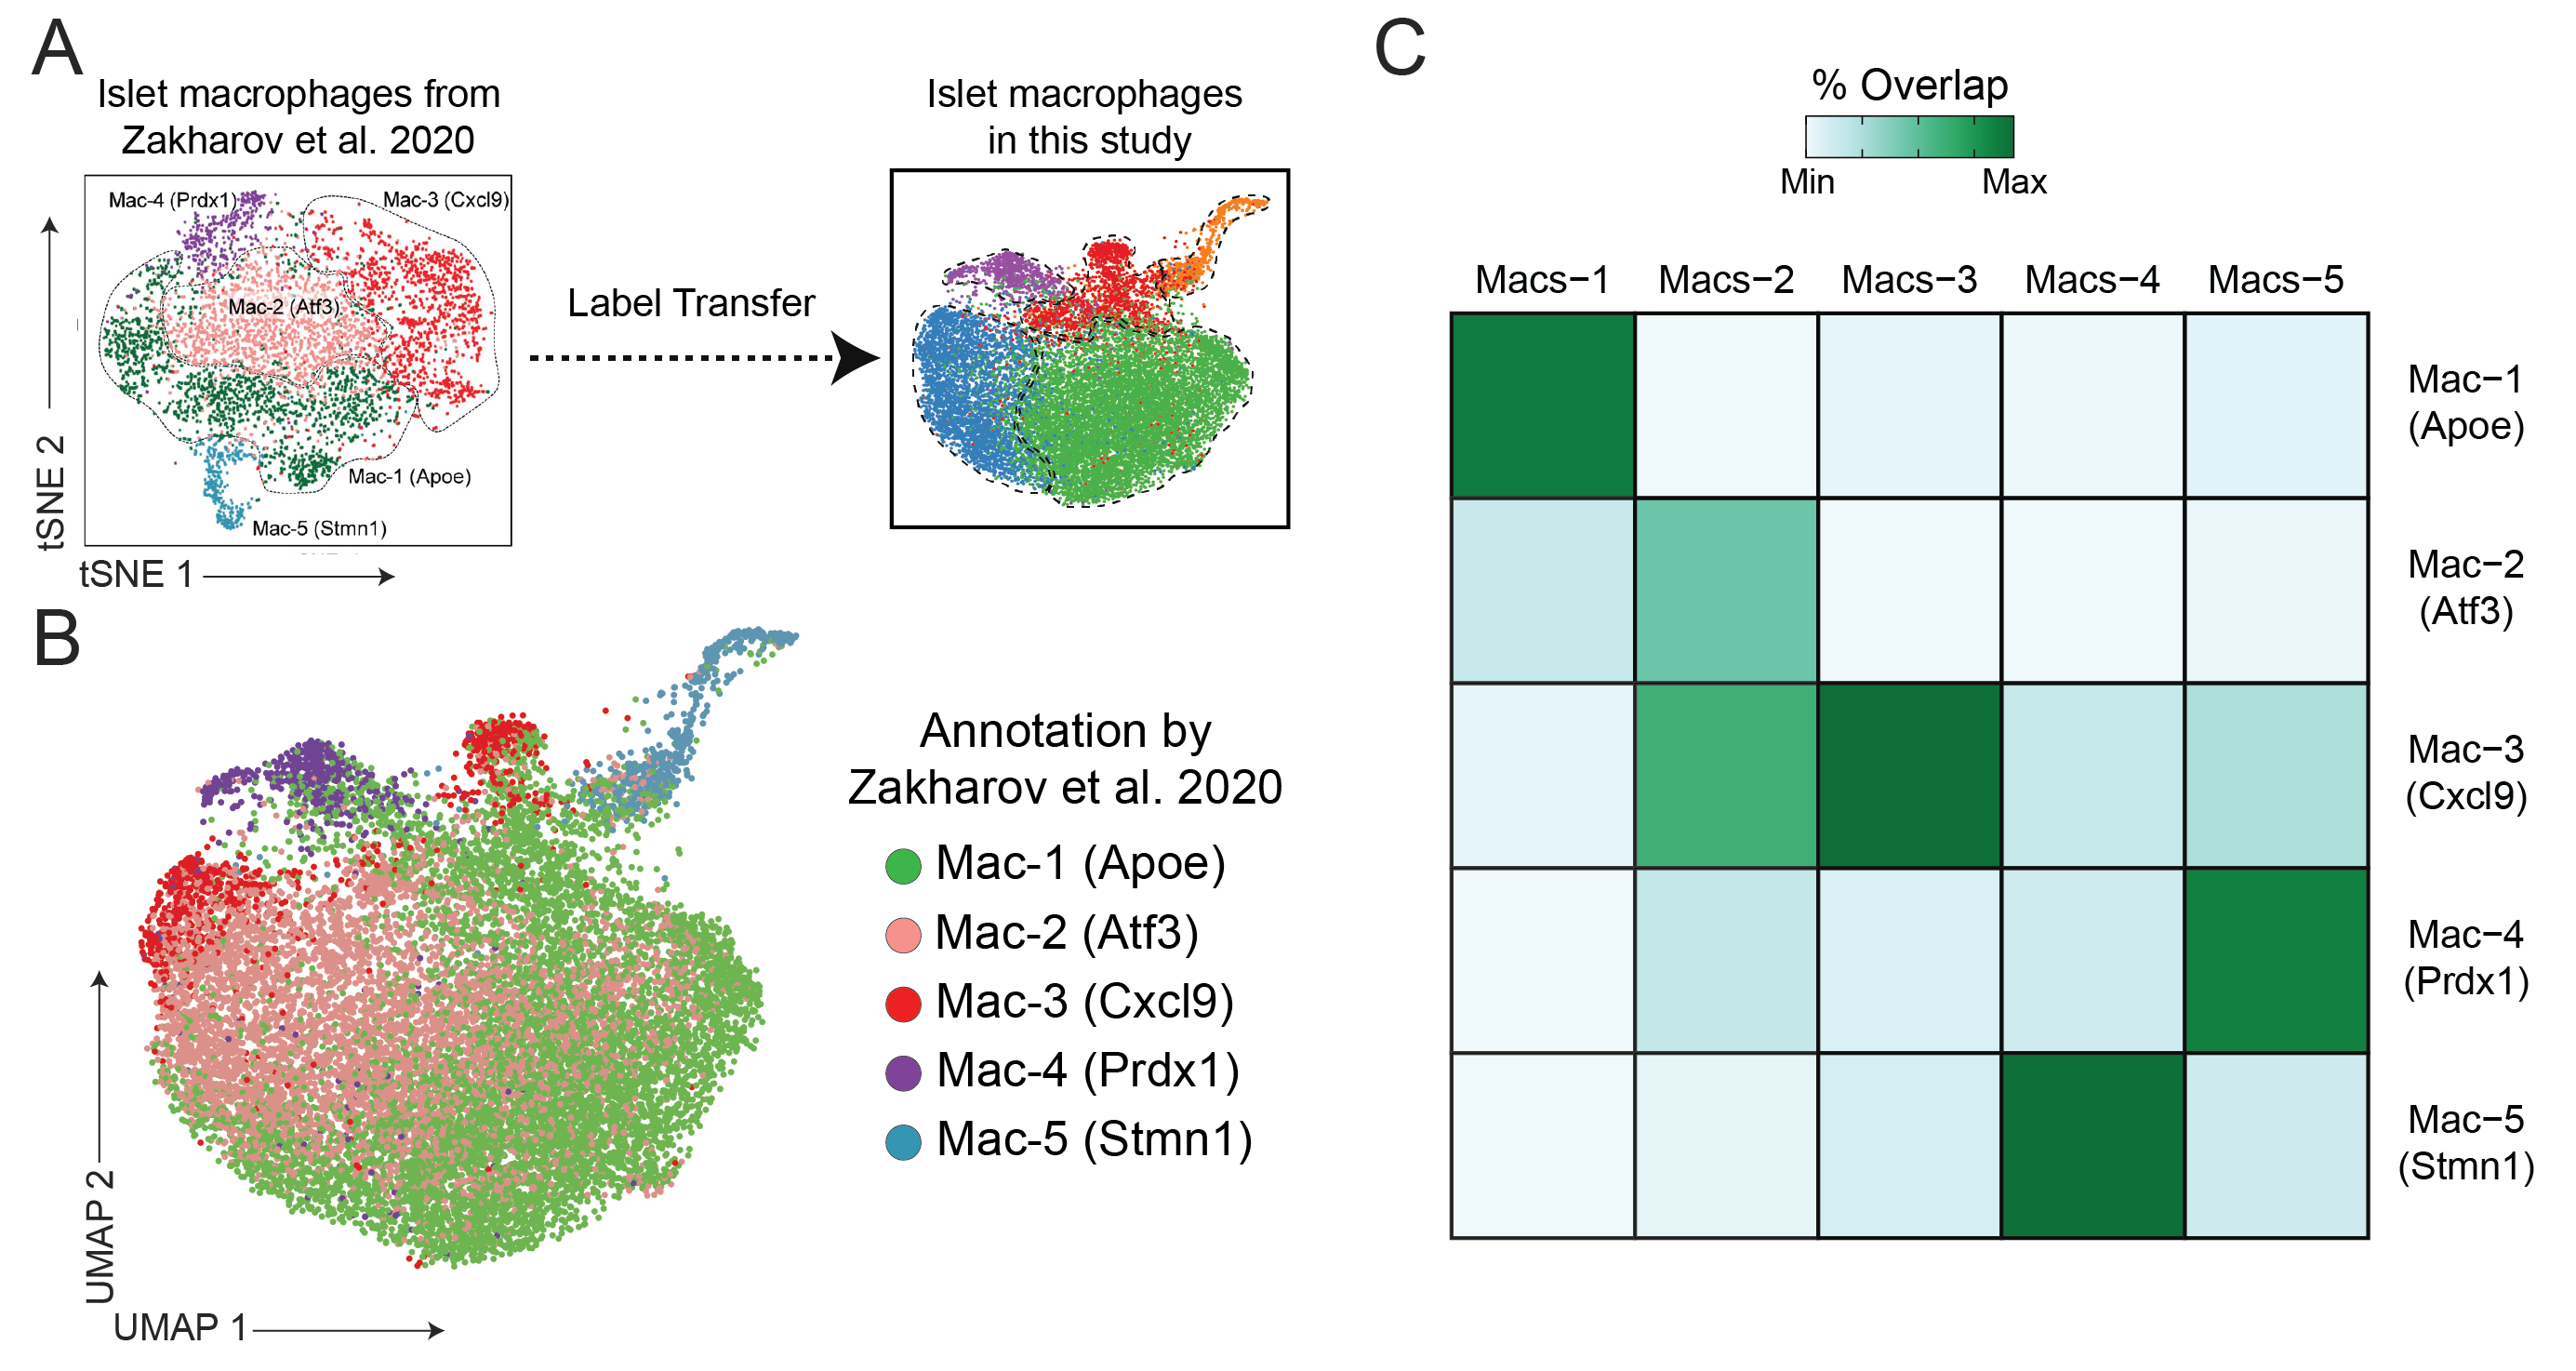
\includegraphics[width=8cm]{Chapter4/Fig/F2-5-02.png}
% \caption[res-macs3]{\textbf{Label transfer of annotations from Zakharov et. al}}
% \label{fig2-5-3}
% \end{wrapfigure}

A similar single-cell study of islet macrophages in a \gls{nod} mouse model identified five main macrophage sub-populations \textbf{\cite{zakharov_single-cell_2020}}. In the study by Zakharov \textit{et al.}, the authors identified a non-inflammatory sub-population, Mac-1 (\textit{Apoe}), characterized by elevated levels of \textit{Apoe} and \textit{Trem2}; two groups of inflammatory activated macrophages, Mac-2 (\textit{Atf3}), characterized by strong \gls{nfkb} activation and elevated expression of genes encoding inflammatory cytokines, and Mac-3 (\textit{Cxcl9}), which depicted elevated expression of genes encoding several cytokines, co-stimulatory molecules, and molecules involved in antigen presentation, alongside \gls{nfkb} signature. Apart from these three groups, the authors also identified Mac-4 (\textit{Prdx1}), associated with lysosomal activity and apoptotic cell clearance and Mac-5 (\textit{Stmn1}), associated with the cell-cycle pathway \textbf{(\autoref{fig:chp2_scrna_macrophages_unanue} A,} left\textbf{)}.\\

% \begin{wrapfigure}{l}{0.5\textwidth}
% \vspace{-20pt}
% 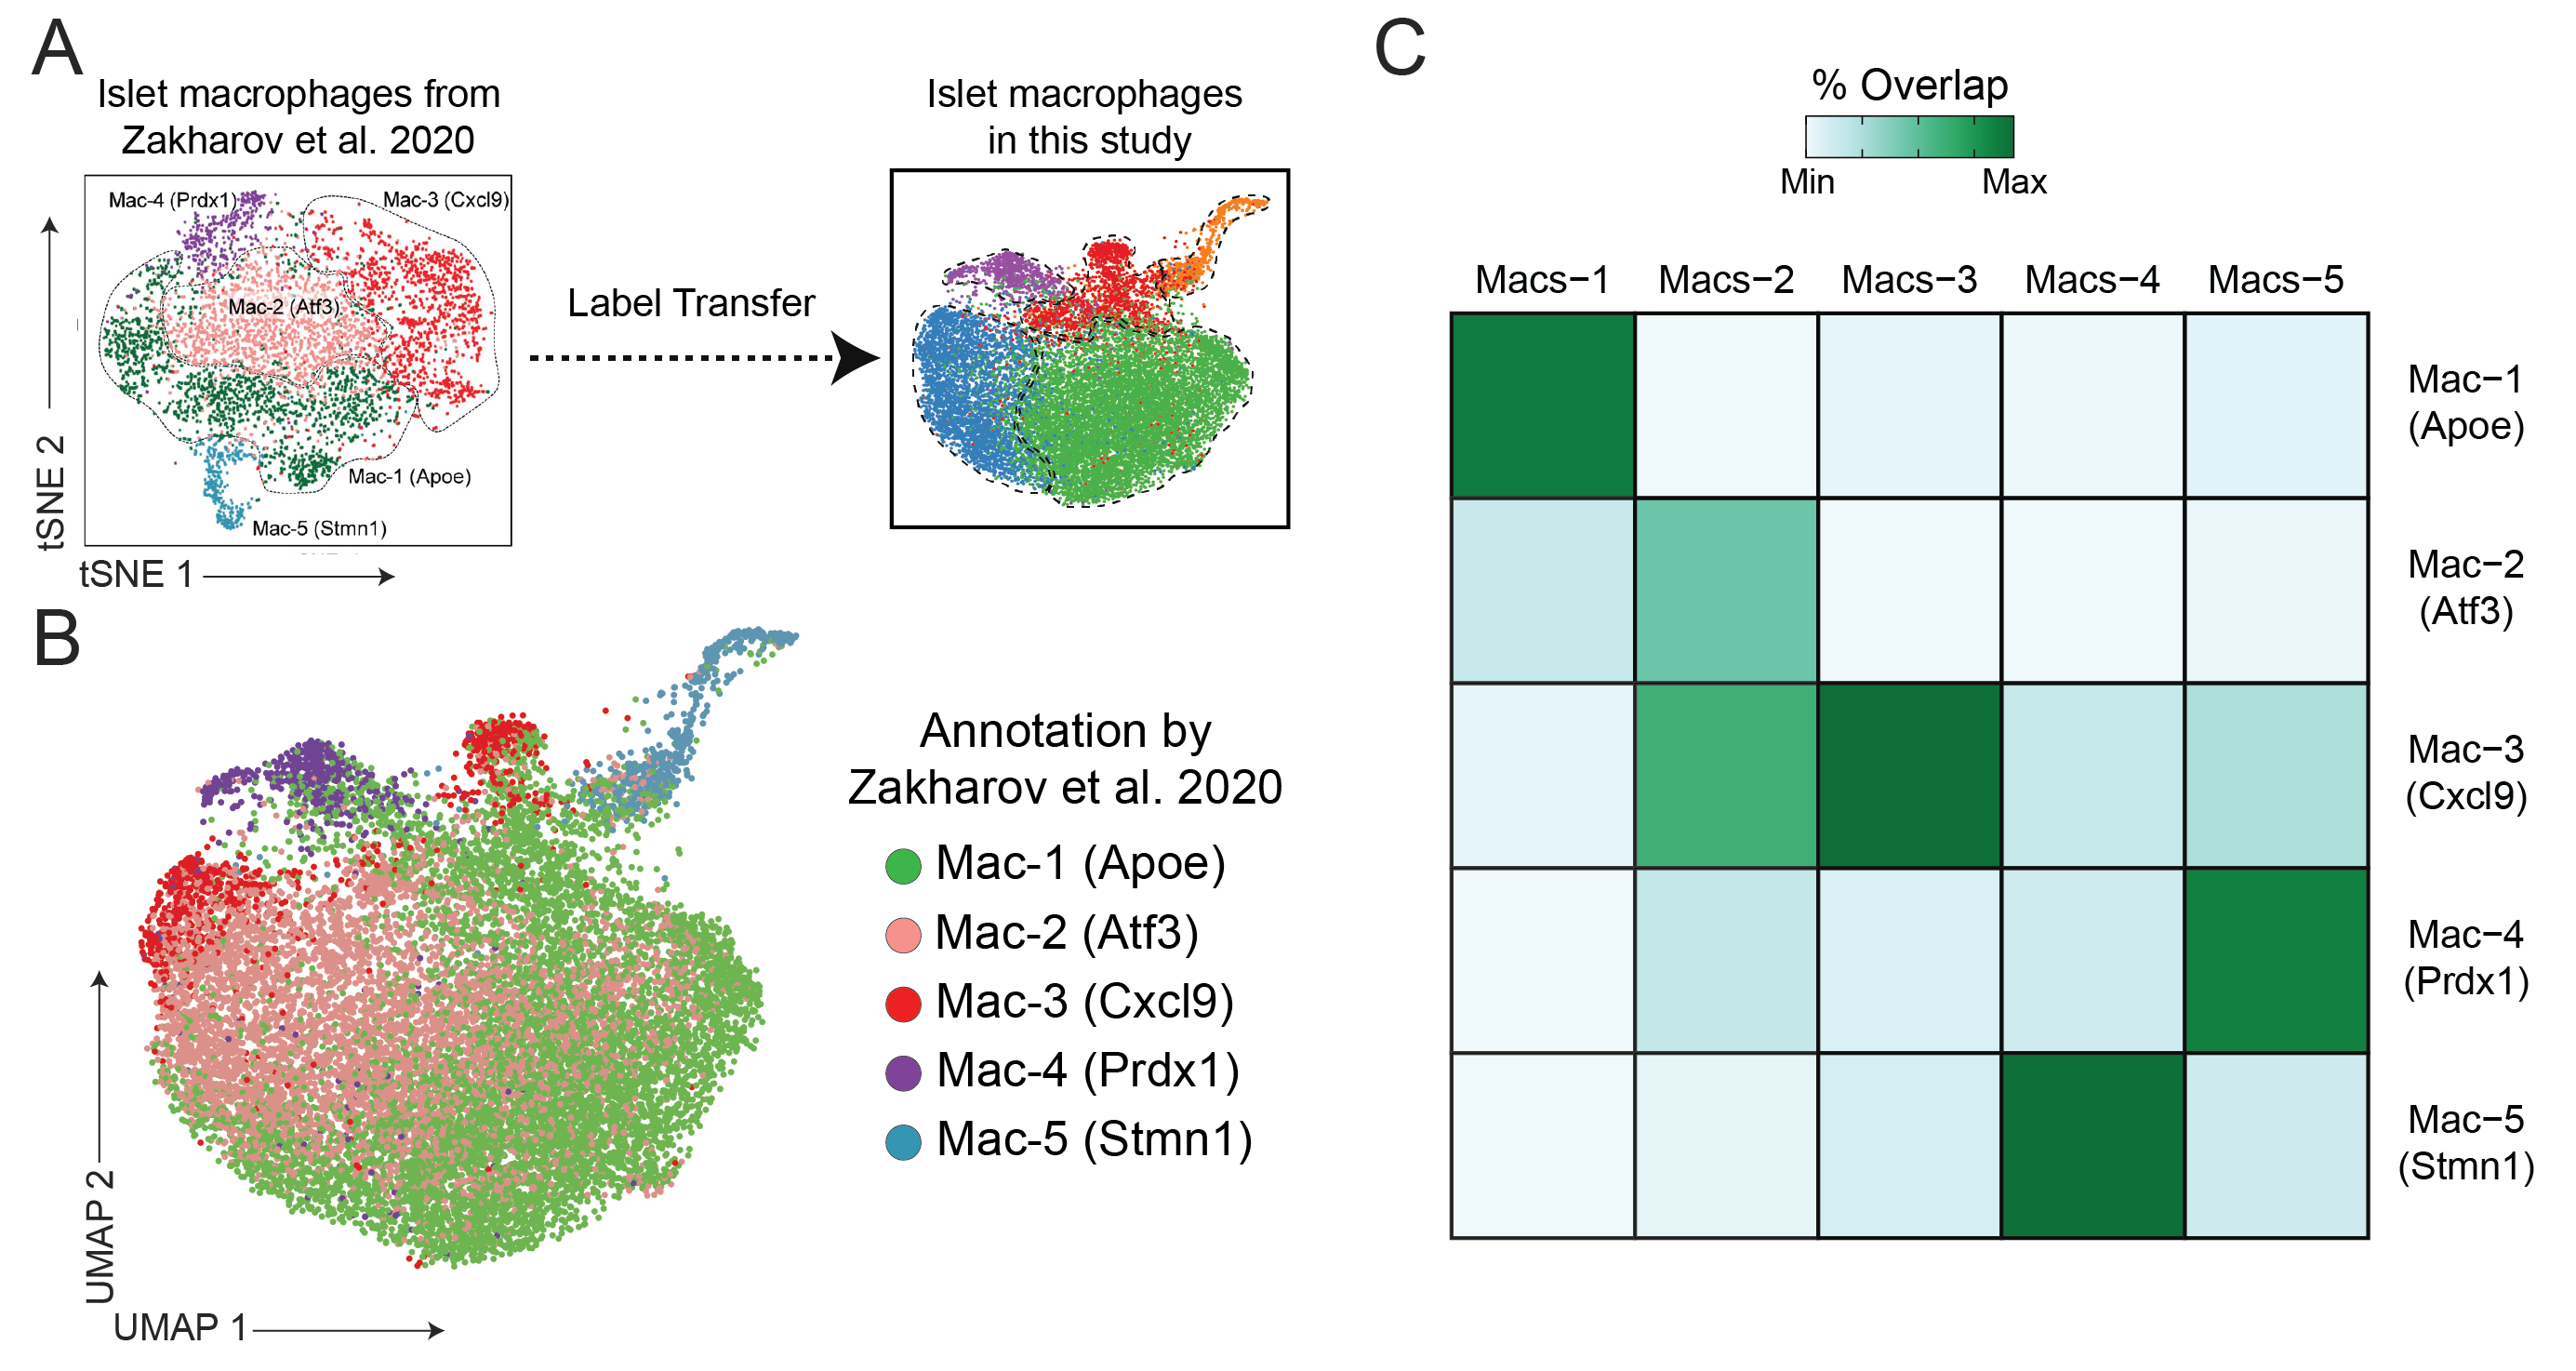
\includegraphics[width=7cm]{Chapter4/Fig/F2-5-02.png}
% \caption[Mapping islet macrophages from flp1{t1d}{T1D} \glslink{nod}{NOD} mice]{\textbf{Mapping islet macrophages from \glslink{t1d}{T1D} \glslink{nod}{NOD} mice.} \textbf{(A) Left:} \gls{tsne} embedding of islet macrophage populations characterized by Zakharov \textit{et al.}, illustrating the five distinct sub-populations. \textbf{(B)} \gls{umap} embedding of islet macrophages from this study, grouped according to annotations in panel \textbf{(A) Left} following the label transfer workflow.}
% \label{fig:chp2_scrna_macrophages_unanue}
% \vspace{-10pt}
% \end{wrapfigure}
\vspace{-20pt}
\begin{figure}[H]
\centering
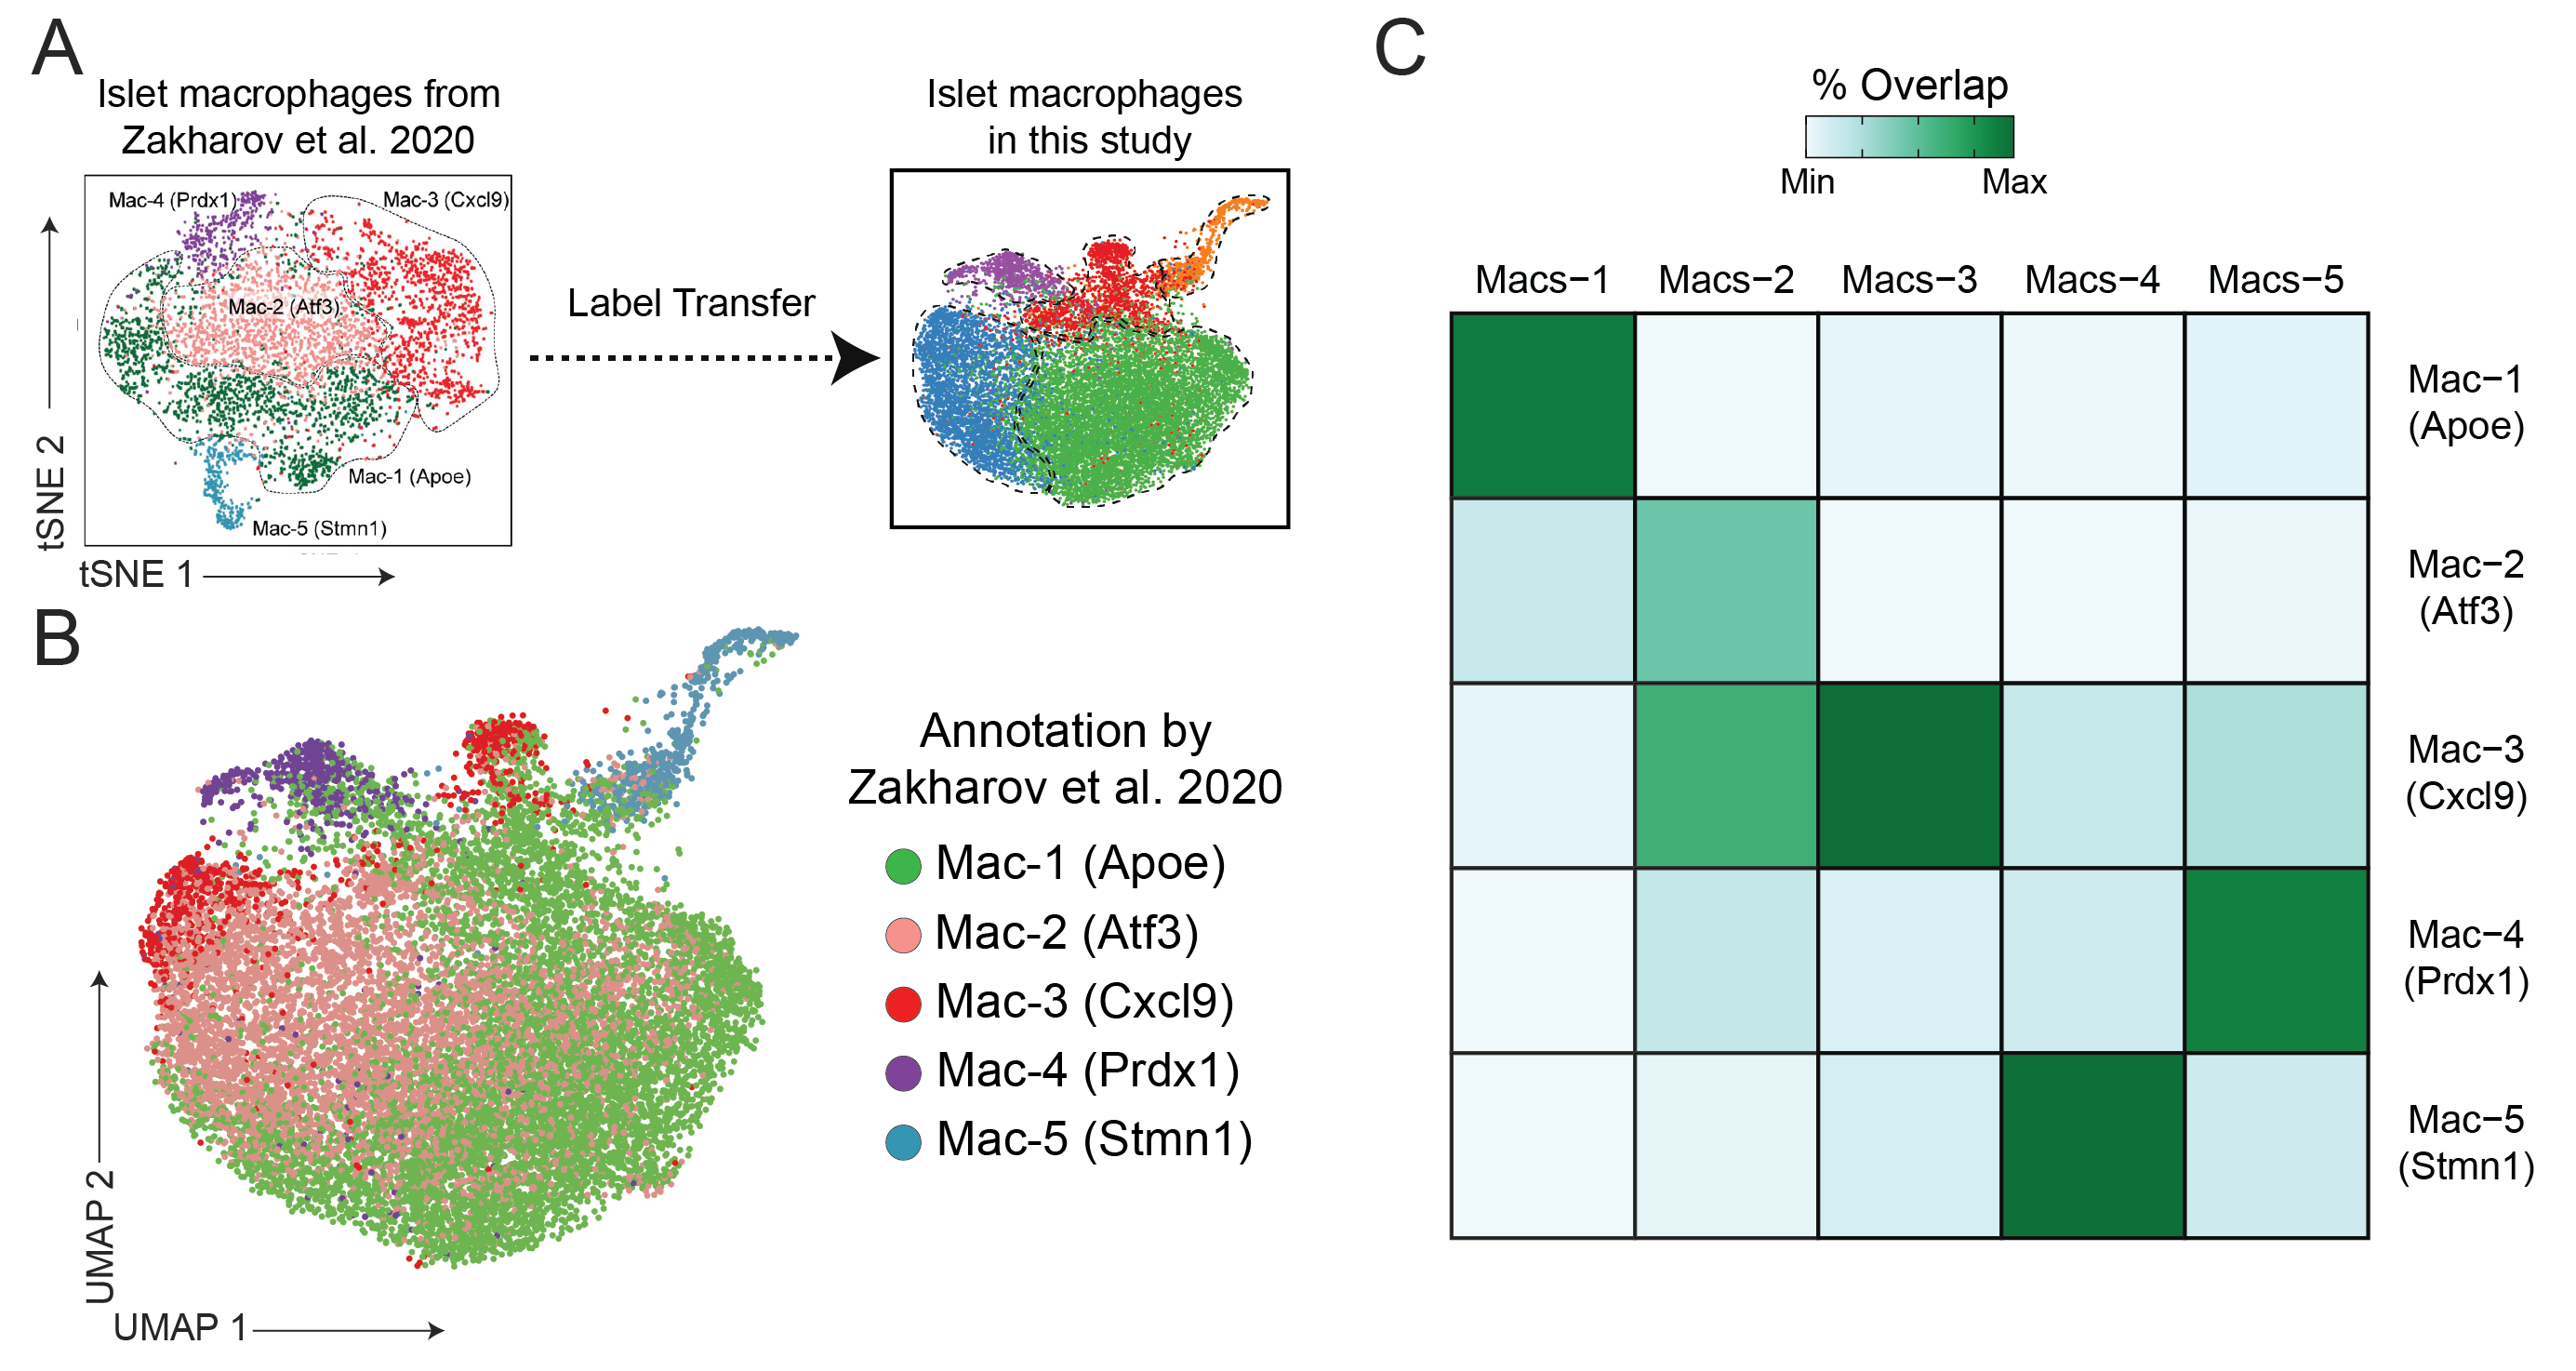
\includegraphics[width=13cm]{Chapter4/Fig/F2-5-02.png}
\caption[Reference-to-query mapping of islet macrophages]{\textbf{Reference-to-query mapping of islet macrophages.} \textbf{(A)} Schematic depicting the label transfer workflow to map the annotations of the islet macrophages in the \gls{nod} model of \gls{t1d} onto the macrophages identified in this study. \textbf{(B)} \gls{umap} embedding of islet macrophages from this study, grouped according to annotations of the \gls{t1d} \gls{nod} mice islet macrophages, following the label transfer workflow. \textbf{(C)} Heatmap depicting the percentage of overlap of marker genes for the \gls{t1d} \gls{nod} mice islet macrophages (rows) and the islet macrophages from this study (columns).}
\label{fig:chp2_scrna_macrophages_unanue}
\end{figure}

\par Therefore, noting the transcriptomic similarities between the islet-intrinsic macrophages in the \gls{nod} model of \gls{t1d} and \gls{wd}-fed mice from our analysis, we performed label transfer and mapped these \gls{nod}-mice macrophage sub-populations onto our islet macrophages \textbf{(\autoref{fig:chp2_scrna_macrophages_unanue} A;} see \hyperref[subsubsec:met_chp2_labeltransfer]{\textbf{Methods}}\textbf{)}. This analysis revealed a strong correspondence in the islet-resident macrophage sub-populations between the two studies \textbf{(\autoref{fig:chp2_scrna_macrophages_unanue} B)}. In addition to this, there was also strong one-to-one overlap of marker genes for the macrophage sub-populations identified in the two studies \textbf{(\autoref{fig:chp2_scrna_macrophages_unanue} C)}. In the original study, Mac-1 and Mac-2 macrophages showed limited changes over time whereas Mac-3 was the only sub-population that showed continuous strong expansion during \gls{t1d} progression \textbf{\cite{zakharov_single-cell_2020}}. This echoes similar observation of limited composition shifts of Macs-1 and Macs-2 macrophages and the expansion of Macs-3 in response to \gls{wd} feeding in our analysis \textbf{(\autoref{fig:chp2_scrna_macrophages} D)}. Additionally, the Mac-3 sub-population was comprised of two distinct groups: a monocyte-derived Mac-3 macrophages which expressed a number of monocyte markers (\textit{Ccr2,Plac8} and \textit{Ly6c1}); and a resident-macrophage developed Mac-3 group which lacked monocytic markers. This heterogeneity within Mac-3 was also apparent upon label transfer as the Mac-3 sub-population mapped partially to Macs-2 and Macs-3 and also in the overlap of the marker genes of the two corresponding sub-populations \textbf{(\autoref{fig:chp2_scrna_macrophages_unanue} B,C)}, with cells in Macs-2 expressing the monocytic marker \textit{Ccr2} \textbf{(\autoref{fig:app_scrna_macrophages_macs2_genes} B)}. Contrary to the decreased proportion of anti-inflammatory Mac-4 during autoimmunity progression, the proportion of the corresponding Macs-5 sub-population was unchanged in response to \gls{wd} feeding or aging \textbf{(\autoref{fig:chp2_scrna_macrophages} D)}.\\

\par In conclusion, the annotation mapping highlighted significant transcriptomic parallels between the islet-intrinsic macrophages in \gls{nod} model of \gls{t1d} and those in \gls{wd}-fed and old mice. 


% to show continuous strong expansion during \gls{t1d} progression



% <ADD MORE SENTENCES>

%\clearpage


\subsubsection{\large Linking macrophage sub-populations from \gls{scr} to \gls{imc}}

To establish a link between the macrophage sub-populations identified in our single-cell analysis and those determined through the \gls{imc} analysis, we examined, in our \gls{scr} dataset, the expression of marker genes corresponding to the \gls{imc} channels used for the classification of macrophages. Our investigation indicated that F4/80 expression was highest in Macs-1, lower in Macs-3, and lowest in Macs-2 \textbf{(\autoref{fig:chp2_scrna_macrophages_imc} A,} top\textbf{)}. Observing a similar pattern in the \gls{imc} analysis, we linked Macs-1, Macs-2, and Macs-3 macrophage sub-populations in the \gls{scr} dataset to the F4/80\textsuperscript{\textit{high}}, F4/80\textsuperscript{-}, and F4/80\textsuperscript{\textit{low}} sub-populations, respectively. Specifically, Macs-3, akin to the F4/80\textsuperscript{\textit{low}} sub-population, showed moderate F4/80 channel (\textit{Adgre1}) expression but exhibited the highest levels of CD11c (\textit{Itgax}) and CD69 (\textit{Cd69}) channel expression as signs of activation \textbf{(\autoref{fig:chp2_scrna_macrophages_imc} B)}. Moreover, the proliferative Macs-4 macrophages likely equates to the KI67\textsuperscript{\textit{high}} macrophages observed in the \gls{imc} analysis \textbf{(\autoref{fig:chp2_scrna_macrophages_imc} A} top\textbf{, B)}. We did not find an equivalent for the Macs-5 sub-population in the preceding \gls{imc} analysis, suggesting possible discrepancies between protein-based and \glsentryshort{rna}-based methodologies for cell type annotation. To further confirm the resemblance between the Macs-3 and F4/80\textsuperscript{\textit{low}} sub-populations, we examined the expression of these marker genes under \gls{wd} feeding and aging conditions. The Macs-3 sub-population manifested an augmented inflammatory phenotype under both conditions, as evidenced by the up-regulated gene expression of CD11c (\textit{Itgax}) and CD69 (\textit{Cd69}) \textbf{(\autoref{fig:chp2_scrna_macrophages_imc} A,} bottom\textbf{)}. This inflammatory modulation parallels observations in the F4/80\textsuperscript{\textit{low}} cells as elucidated from the \gls{imc} analysis \textbf{(\autoref{fig:chp2_scrna_macrophages_imc} C)}.\\


\begin{figure}[t!]
\centering
%\vspace{-25pt}
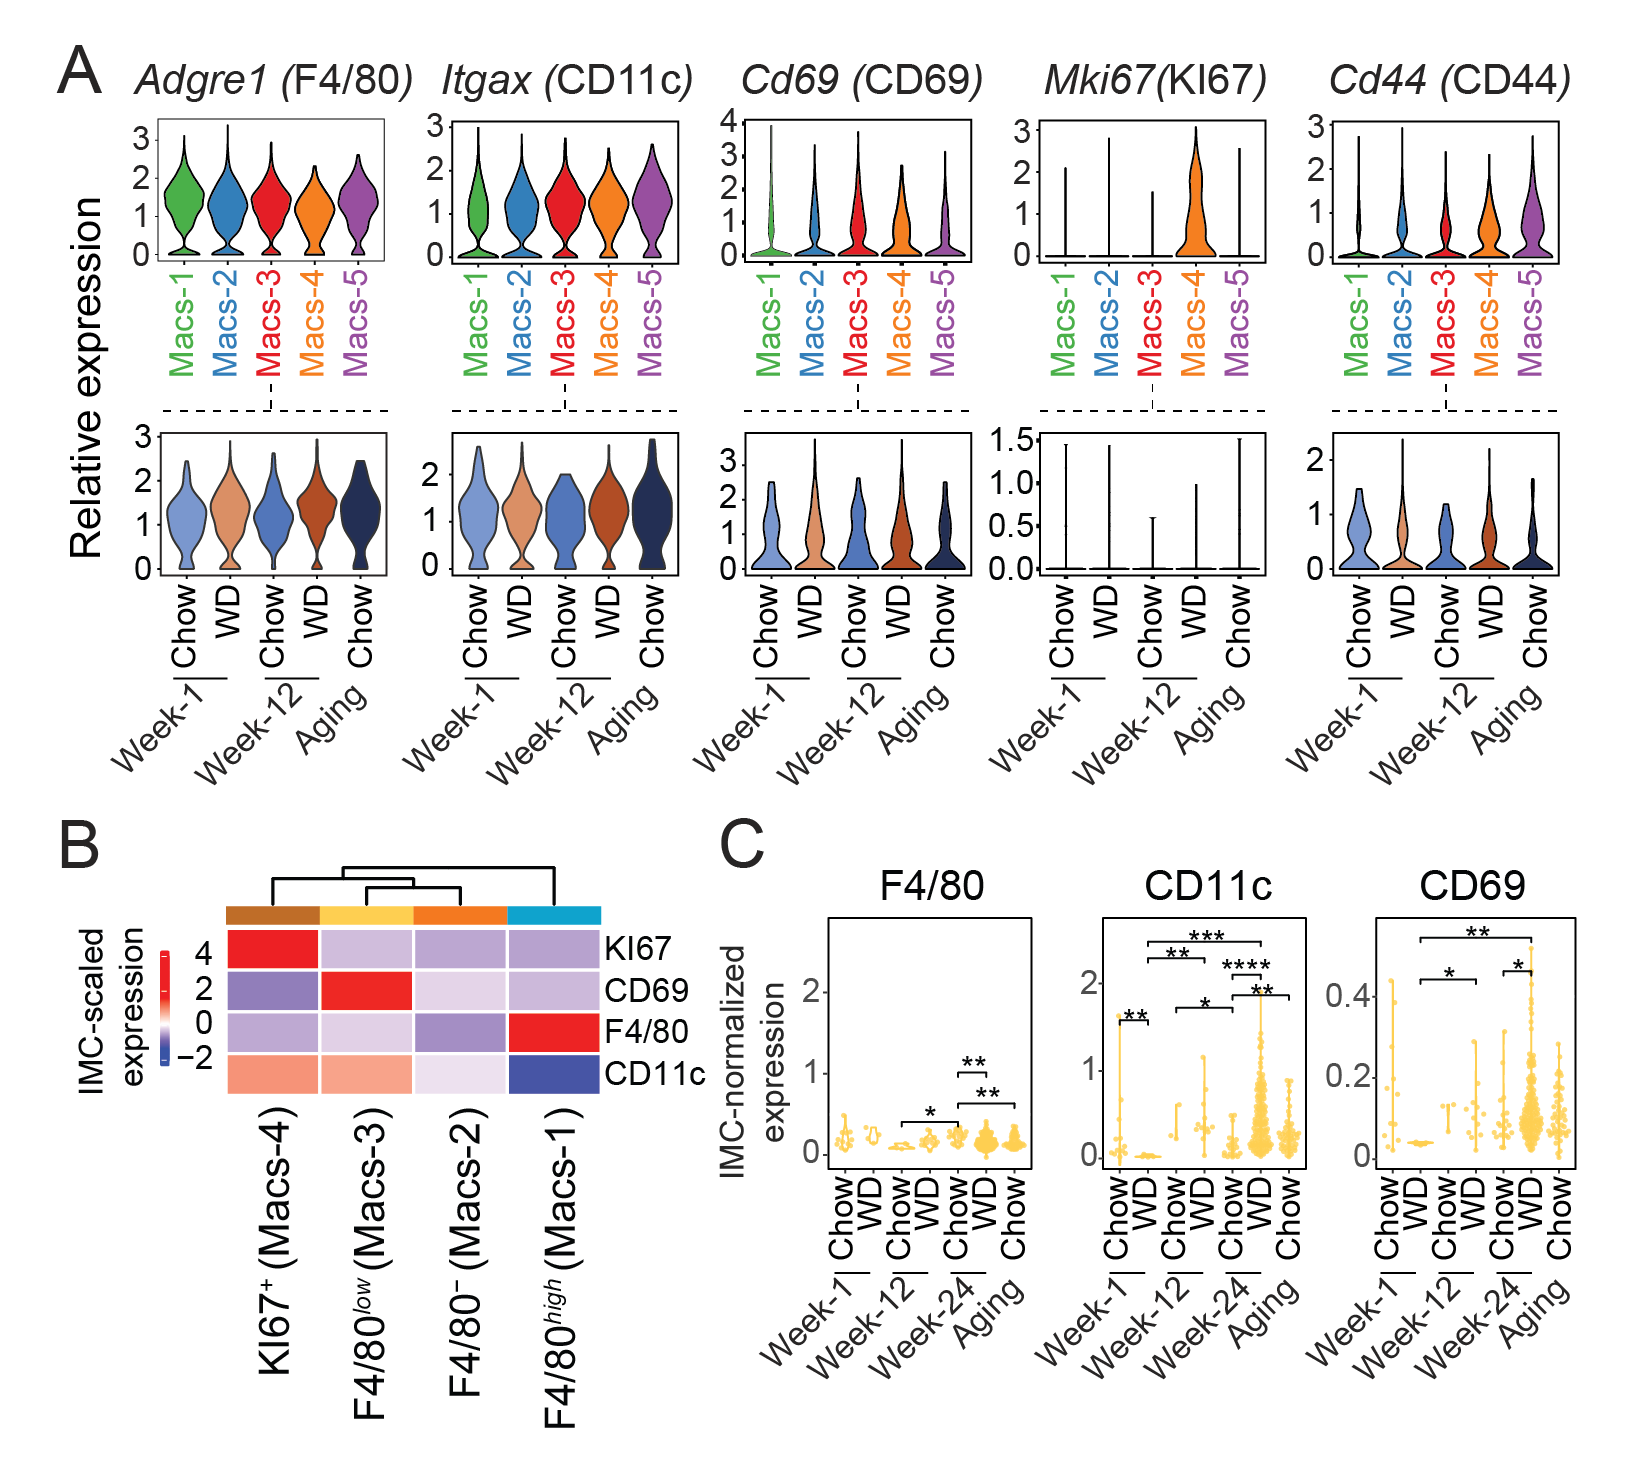
\includegraphics[width=\linewidth]{Chapter4/Fig/F2-4-01.png}
\caption[Linking macrophage sub-populations from \glsentryshort{scr} to \glsentryshort{imc}]{\textbf{Linking macrophage sub-populations from \gls{scr} to \gls{imc}.} \textbf{(A)} Violin plots depicting the normalized expression levels of genes with corresponding channels in the \gls{imc} panel. The top row depicts the expression across various macrophage sub-populations, and the bottom row depicts their expression in the Macs-3 sub-population under across the experimental groups. \textbf{(B)} Heatmap showing \textit{z-score} expression of selected \gls{imc} channels across the four macrophage sub-populations identified in the \gls{imc} analysis. Corresponding macrophage sub-populations from \gls{scr} data are indicated in parentheses. \textbf{(C)} Violin plots of \textit{arcsinh} transformed expression of selected channels in the F4/80\textsuperscript{\textit{low}} macrophage sub-population from the \gls{imc} analysis across the experimental groups. $\textsuperscript{*} p < 0.05, \textsuperscript{**} p < 0.01, \textsuperscript{***} p < 0.001 and \textsuperscript{****} p < 0.0001$. p-values were calculated using the Wilcoxon rank-sum test with Bonferroni correction. \textit{The data and figure in } \textbf{(B)} \textit{and} \textbf{(C)} \textit{were originally generated by Dr. Matthias Barone and reused here with permission.}}
\label{fig:chp2_scrna_macrophages_imc}
\end{figure}




\par Collectively, we identified macrophage sub-populations with distinct activation status in the pancreatic islets. Our findings underscore age-related accumulation and activation of inflammatory Macs-3 (F4/80\textsuperscript{\textit{low}}) macrophages within pancreatic islets, a phenomenon that is markedly amplified under over-nutrition conditions.

%\clearpage

% \mysidecaption{0.4}{%
% \captionof{figure}{\textbf{Linking macrophage sub-populations between scRNA-seq and IMC analyses.} \textbf{(A)} Violin plots depicting the normalized expression levels of selected markers with corresponding channels in the IMC panel. The top plots compare these levels across various macrophage sub-populations, and the bottom plots display their expression in the Macs-3 population under different experimental conditions. \textbf{(B)}Heatmap showing z-scored expression of selected IMC channgels across the four macrophage sub-populations identified in the IMC analysis. Corresponding macrophage sub-populations from scRNA-seq analysis are indicated in parantheses. \textbf{(C)} Violin plots of \textit{arcsinh} transformed expression of selected IMC channels in the F4/80\textsuperscript{\textit{low}} macrophage sub-population from the IMC analysis across experimental conditions. * p<0.05, ** p<0.01, *** p<0.001 and **** p<0.0001. p-values were calculated using the Wilcoxon rank-sum test with Bonferroni correction.}%
% }
% {%
% 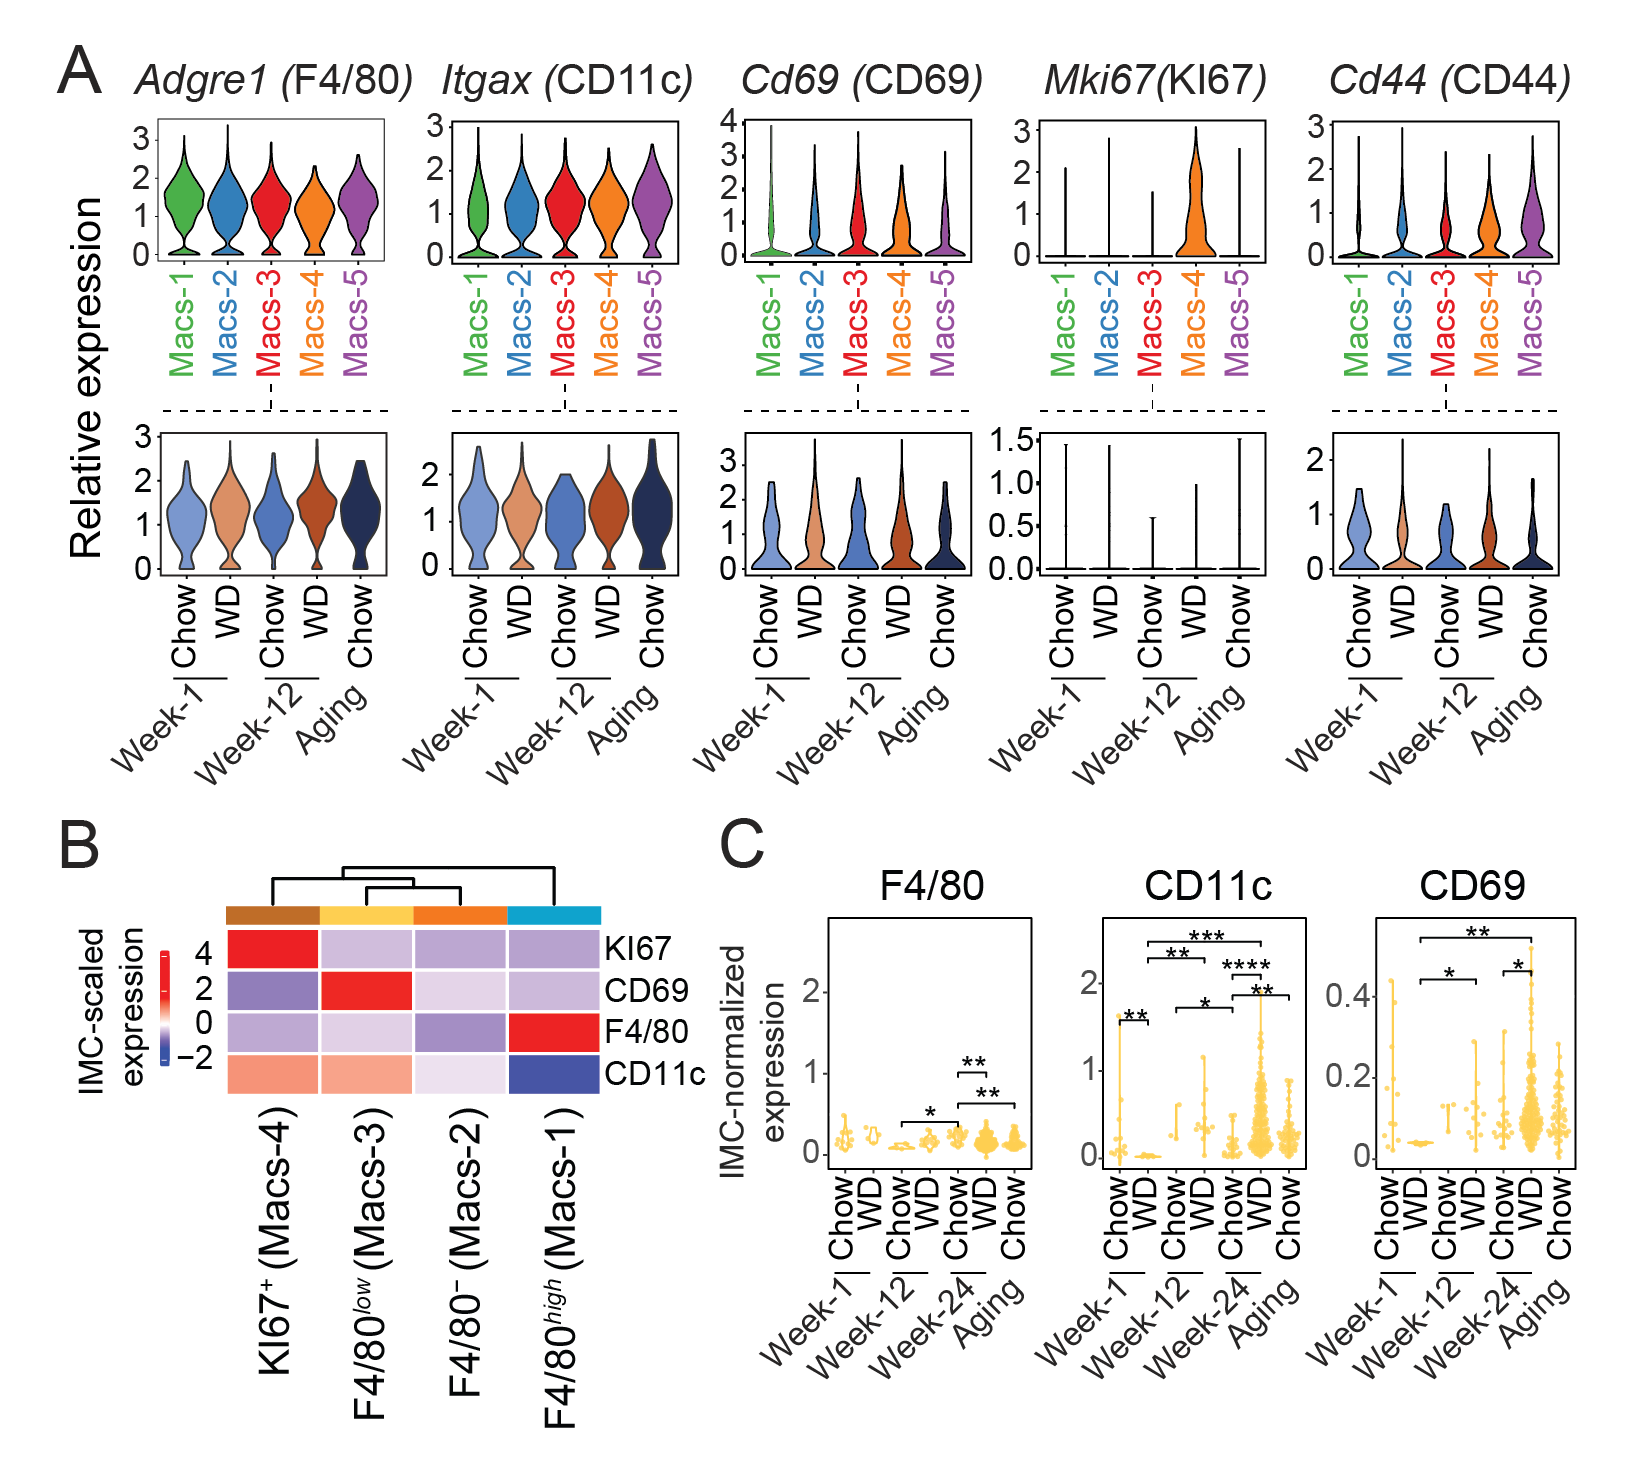
\includegraphics[width=9cm,height=11cm,keepaspectratio]{Chapter4/Fig/F2-4-01.png}%
% }[t]%

% \begin{wrapfigure}{r}{0.5\textwidth}
% 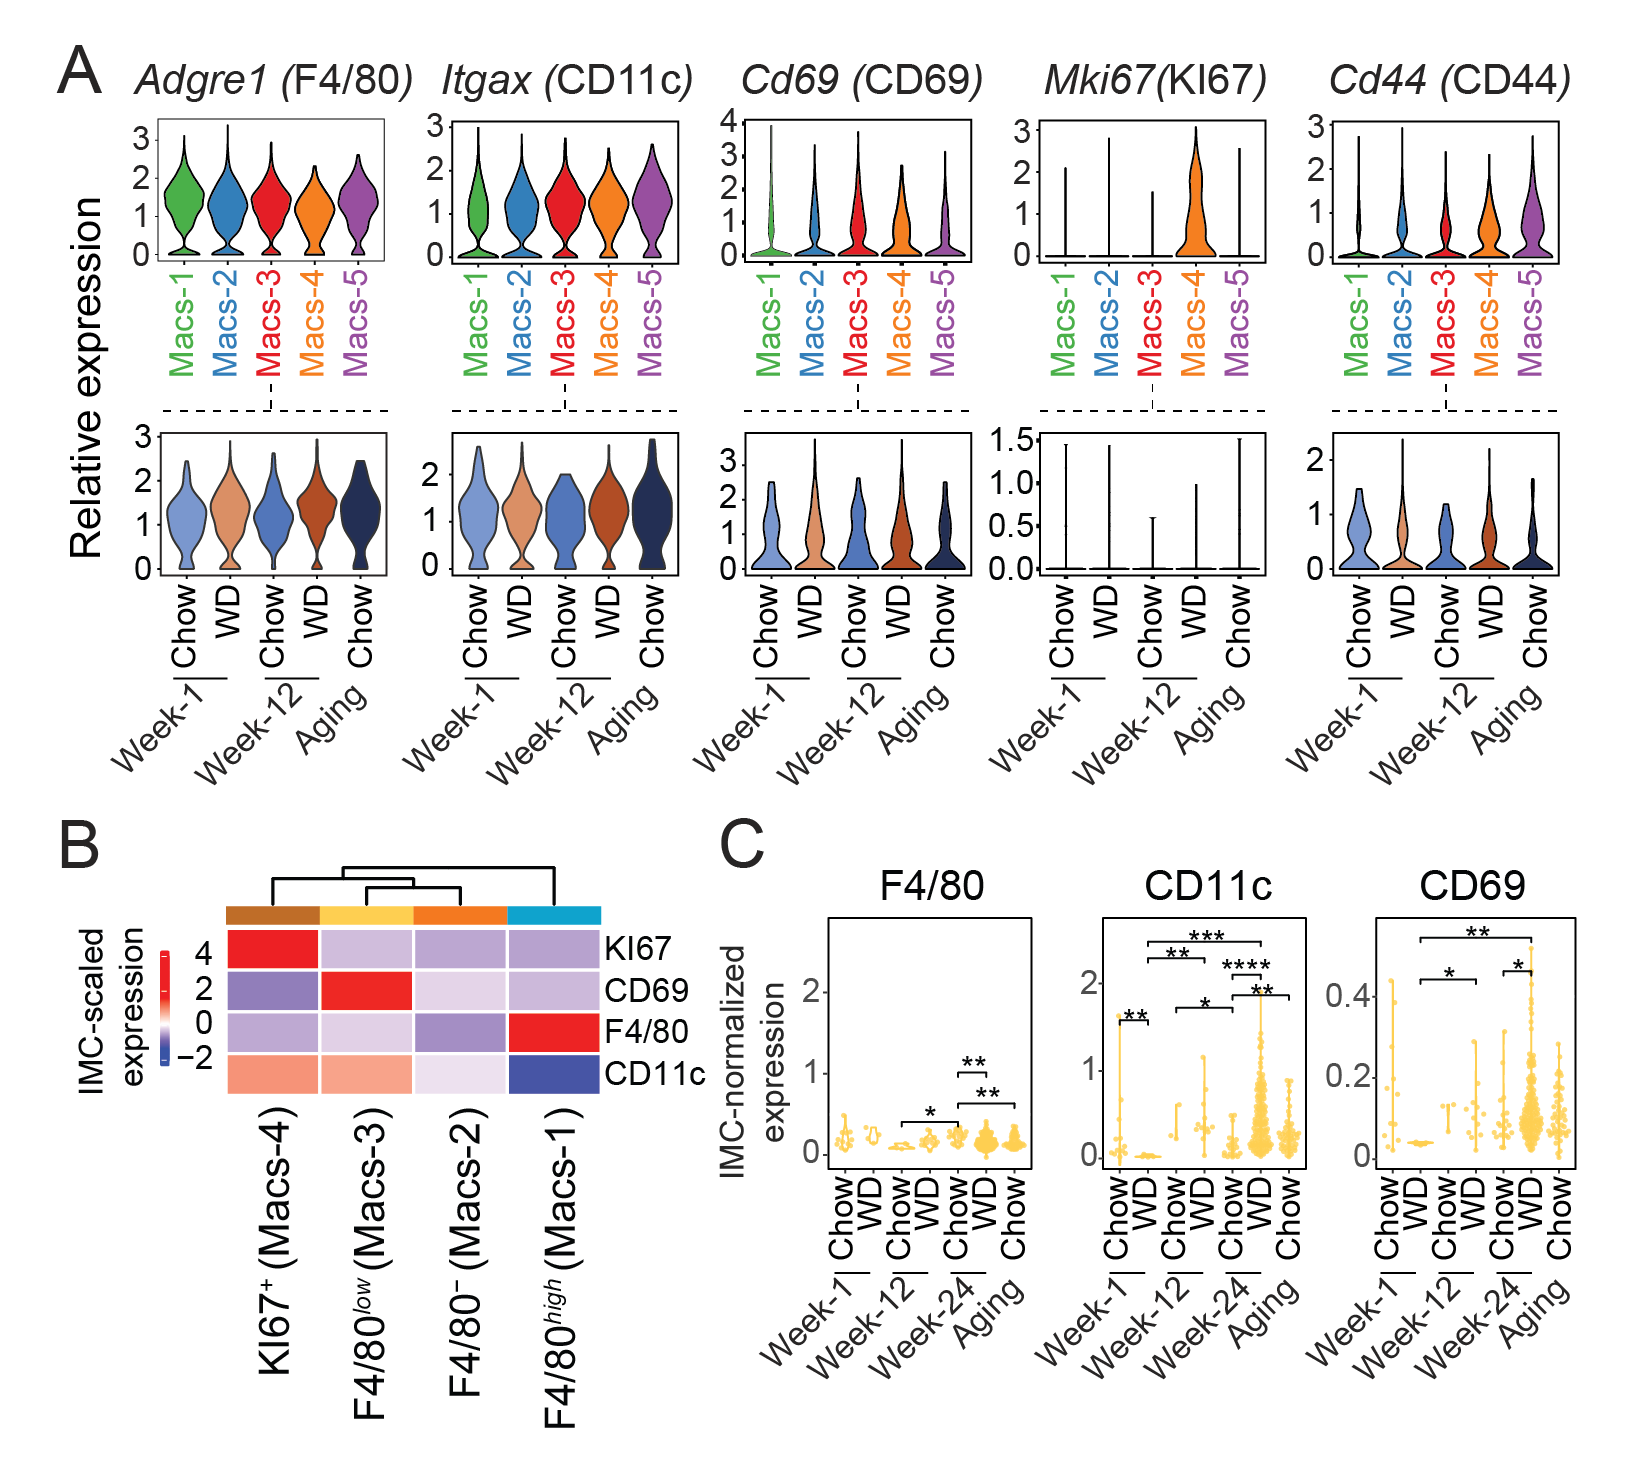
\includegraphics[width=9cm,height=11cm,keepaspectratio]{Chapter4/Fig/F2-4-01.png}
% \caption[]{\textbf{Linking macrophage sub-populations between scRNA-seq and IMC analyses.}}
% \label{fig2-4}
% \end{wrapfigure}

% \begin{SCfigure}[][h]
% \centering
% 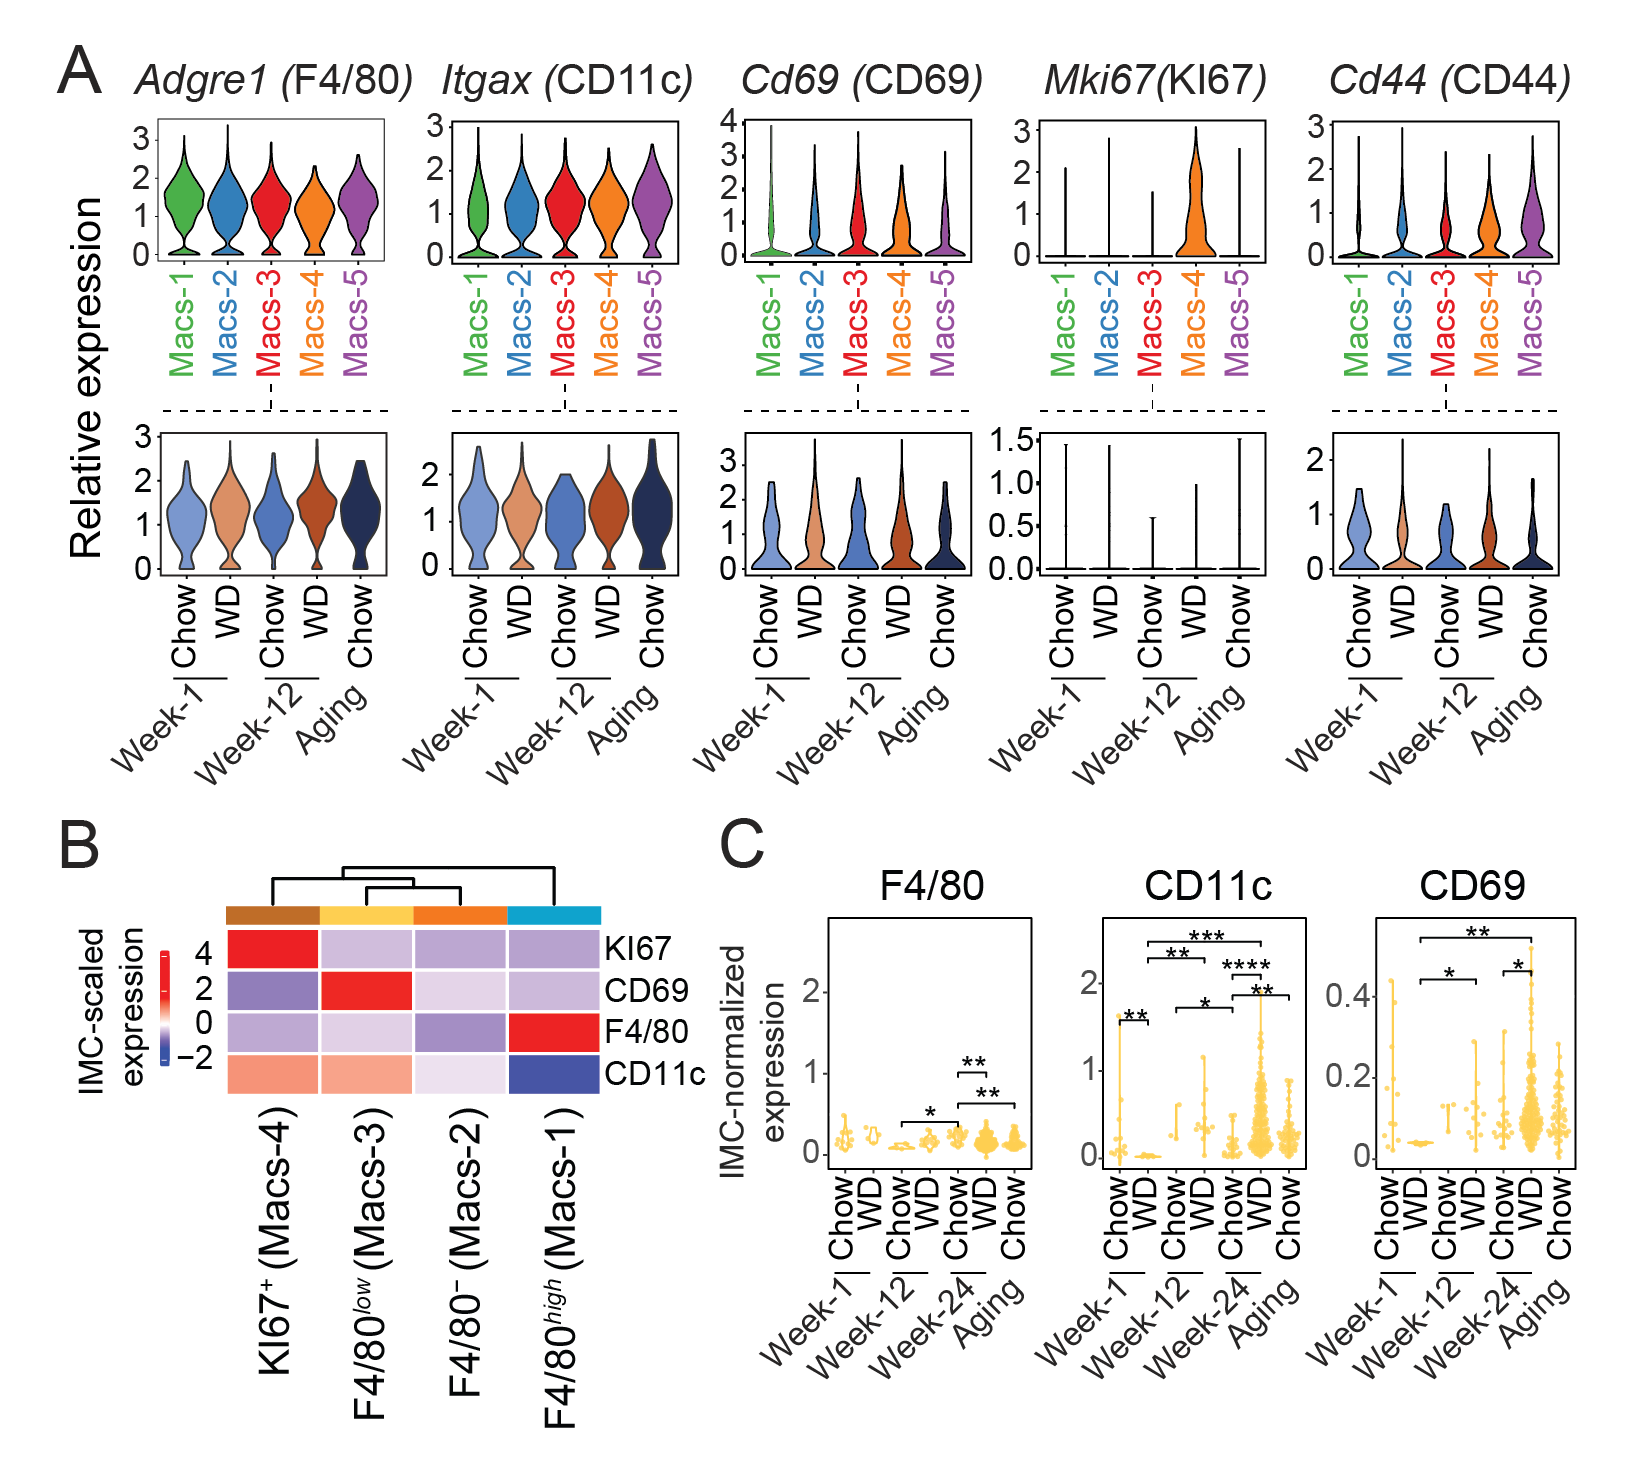
\includegraphics[width=8cm]{Chapter4/Fig/F2-4-01.png}
% \caption[res-macs2]{\textbf{Linking macrophage sub-populations from scRNA-seq to IMC}\\
% \textbf{(A)} Violin plots depicting the normalized expression levels of genes with corresponding channels in the IMC panel. The top plots compare these levels across various macrophage sub-populations, and the bottom plots display their expression in the Macs-3 population under different experimental conditions. \textbf{(B)}Heatmap showing z-scored expression of selected IMC channgels across the four macrophage sub-populations identified in the IMC analysis. Corresponding macrophage sub-populations from scRNA-seq analysis are indicated in parantheses. \textbf{(C)} Violin plots of \textit{arcsinh} transformed expression of selected IMC channels in the F4/80\textsuperscript{\textit{low}} macrophage sub-population from the IMC analysis across experimental conditions. *p<0.05, **p<0.01, ***p<0.001 and ****p<0.0001. p-values were calculated using the Wilcoxon rank-sum test with Bonferroni correction.} 
%  \label{fig2-4}
% \end{SCfigure}

% \begin{SCfigure}[1][h]
% \centering
% \caption[res-macs2]{\textbf{Linking macrophage sub-populations from scRNA-seq to IMC}. \textbf{(A)} Violin plots depicting the normalized expression levels of selected markers with corresponding channels in the IMC panel. The top plots compare these levels across various macrophage sub-populations, and the bottom plots display their expression in the Macs-3 population under different experimental conditions. \textbf{(B)}Heatmap showing z-scored expression of selected IMC channgels across the four macrophage sub-populations identified in the IMC analysis. Corresponding macrophage sub-populations from scRNA-seq analysis are indicated in parantheses. \textbf{(C)} Violin plots of \textit{arcsinh} transformed expression of selected IMC channels in the F4/80\textsuperscript{\textit{low}} macrophage sub-population from the IMC analysis across experimental conditions. * p<0.05, ** p<0.01, *** p<0.001 and **** p<0.0001. p-values were calculated using the Wilcoxon rank-sum test with Bonferroni correction.
% }
% 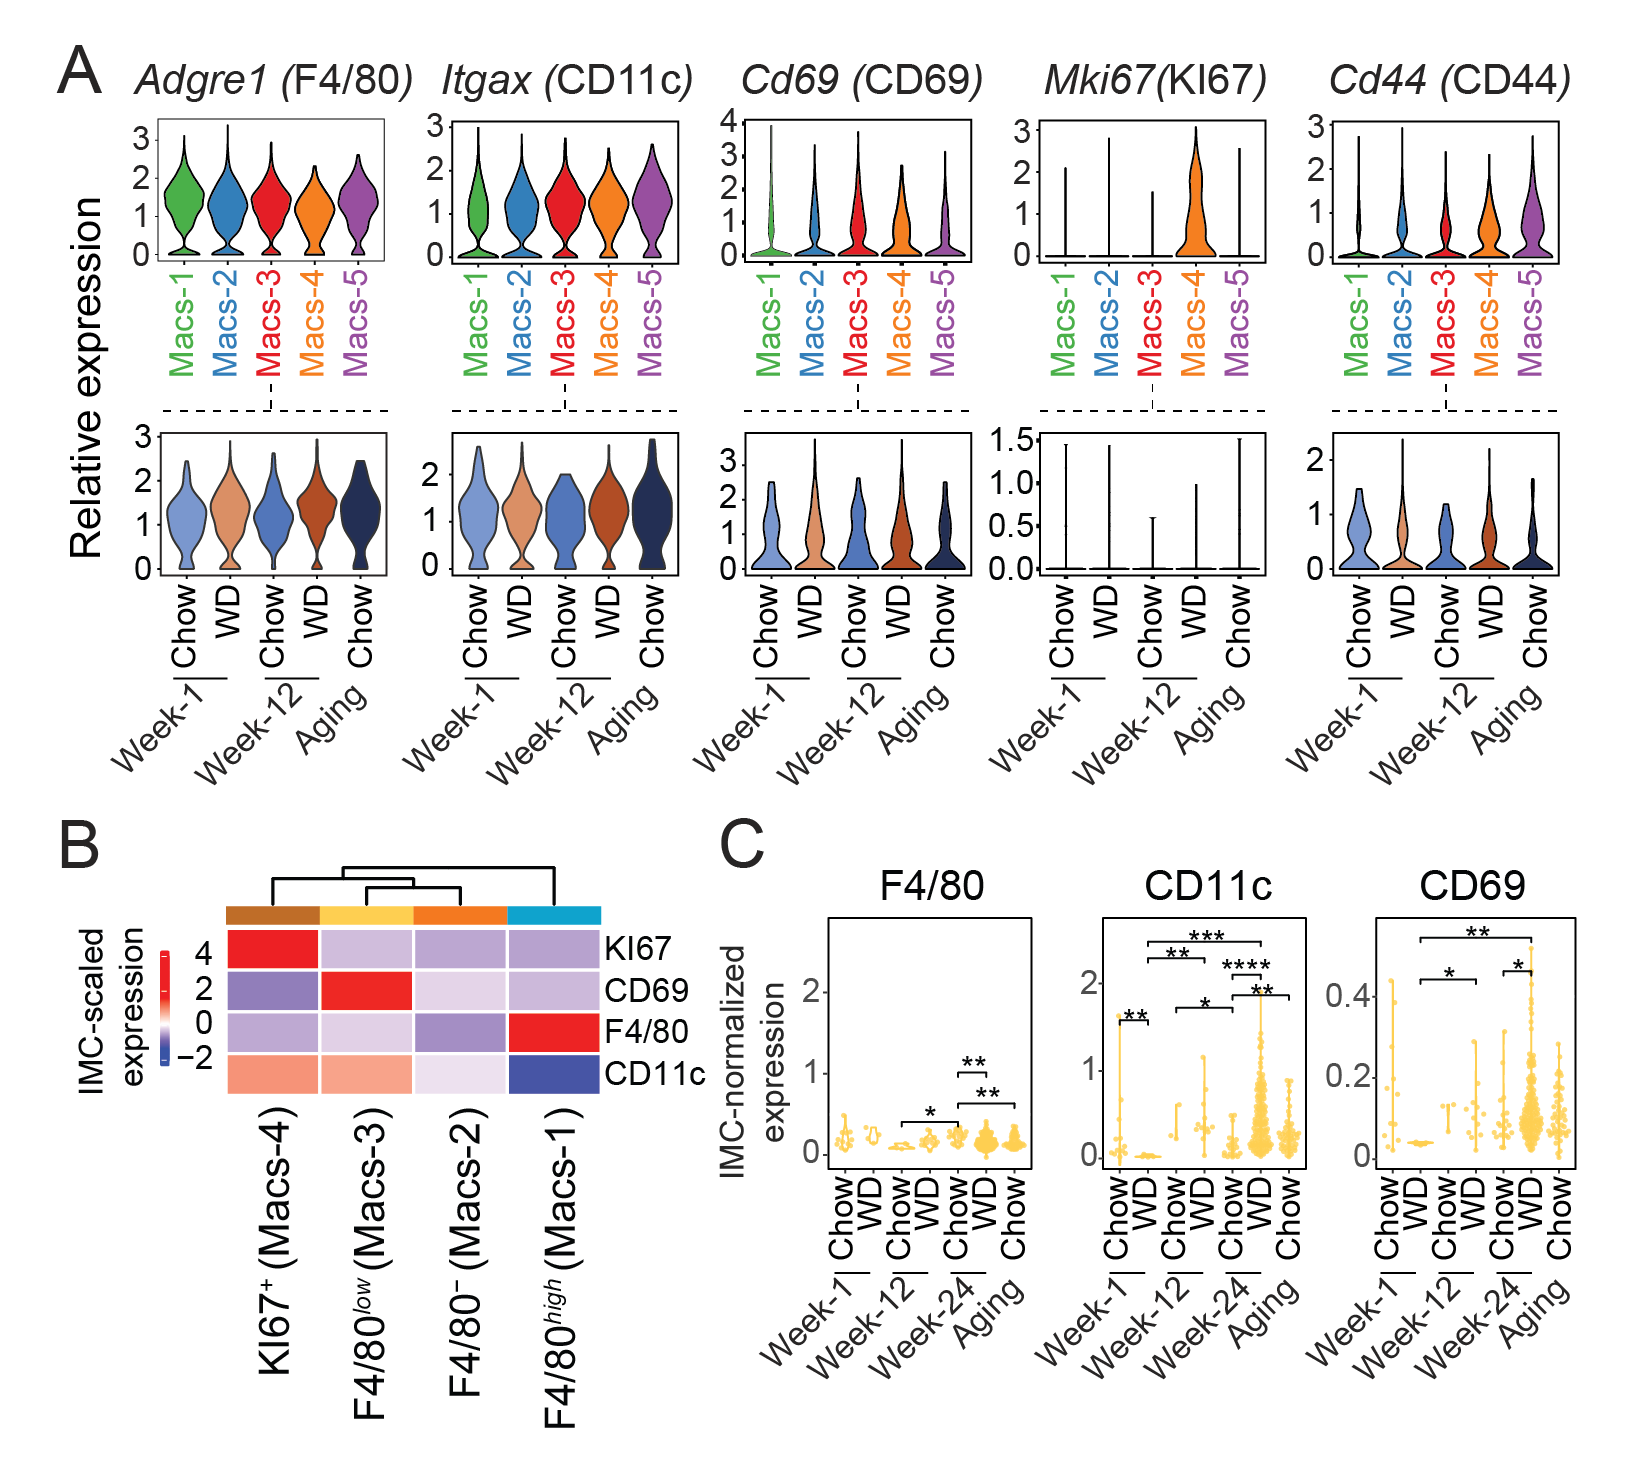
\includegraphics[width=0.6\textwidth]{Chapter4/Fig/F2-4-01.png}
% \label{fig2-4}
% \end{SCfigure}
% \subsubsection{Demultiplexing donors from pooled experiments} 
% \st{Interestingly, despite Macs-2 exhibiting a lower activation profile compared to Macs-3, WD feeding resulted in a stronger expression of genes coding for inflammatory cytokines and chemokines in Macs-2 (Figure S4D,E). In contrast, this induced upregulation of cytokine genes observed in Macs-2 under WD feeding conditions is not evident in the aging condition (Figure S4F)}


% In the considered pooled experimental design, cells from multiple donors are differentiated together in the same experiment. 
% To be able to link the genetic background of an individual with their transcriptional profile we need to map the cells back to their donor of origin, without the use of any barcode.
% Indeed, we find that for the large majority of cells the RNA-seq reads map to a sufficient number of common genetic variants for us to reliably assign each cell to its original donor.
% In particular, assignment of cells to donors was performed using Cardelino \cite{mccarthy2020cardelino}. 
% In short, Cardelino estimates the posterior probability of a cell originating from a specific donor using common genetic variants in \gls{scrnaseq} reads, while employing a Bayesian beta binomial-based approach to account for technical factors such as differences in read depth, allelic drop-out, and sequencing accuracy. 
% To perform donor assignment, we considered a larger set of \gls{hipsci} lines with genotype information (n=490), including the 126 lines used in this study. 
% A cell's assignment to a donor was considered successful if the model identified the match i) with posterior probability > 0.9, and ii) using a minimum of 10 informative variants. 
% Cells for which the donor identification was not successful were discarded and not considered for further analyses.
% Across the entire dataset, 99\% of cells that passed RNA QC steps (see below) were successfully assigned to a donor.
% In some cases, unexpected donor assignment (where several cells from one experiment were found to be assigned to none of the 4-6 donors used in that experiment) allowed me to identify (and correct) plate swaps that happened in the lab, without losing any data (\textbf{Fig. \ref{fig:plate_swap}}).

% \begin{figure}[h]
% \centering
% \includegraphics[width=14cm]{Chapter4/Fig/cardelino_example.png}
% \caption[Demultiplexing donors]{\textbf{Demultiplexing donors}.\\
% Example of how donor assignment of cells helped identifying a plate swap.
% To explore the results of the donor assignment algorithm \cite{mccarthy2020cardelino}, I plotted cells along two axes: on the x axis, the posterior probability of being assigned to a certain donor, on the y the number of common variants found on \gls{scrnaseq} reads used to perform the assignment.
% Because we know for each experiment which lines are supposed to have been differentiated, we can colour cells based on whether the donor they have been assigned to was used in the specific experiment or not.
% On the left, an example of a correct donor assignment: most cells are assigned to one of the correct donors\footnotemark and the few that are not had very few usable genetic variants.
% On the right, the donor assignment is apparently incorrect.
% Most cells were assigned to donors that were not differentiated in the experiment, in many cases with a high level of confidence and using many variants, which would generally indicate high quality cells.
% Indeed, investigating further we realised that all cells were assigned to donors that all belonged to the same experiment, but that it was a different experiment.
% The wrong label was assigned in the lab: run 225216 actually contained cells from experiment 43 and not 39.
% By resolving this computationally, we avoided mistakes and retained all of the cells from this sequencing run, which would have otherwise been discarded.}
% \label{fig:plate_swap}
% \end{figure}


%\subsubsection{Flow cytometry}

% The success of the differentiation protocol was validated using expression of two protein surface markers, a pluripotency marker, Tra-1-60, and a marker of definitive endoderm, CXCR4. 
% We note that while cells were gated using the two markers, we did not discard any cells based on their expression. 
% In contrast, the first cell QC step performed using \gls{facs} consisted in identifying dead cells based on 7AAD\footnote{Staining with 7AAD is used a cell viability assay.
% 7AAD cannot readily pass through intact cell membranes, thus only cells with compromised membranes will stain.} using \gls{facs} staining.
% These were discarded and were not plated. 
% \gls{facs} data were analysed using the openCyto package, implemented in R \cite{finak2014opencyto}.
% The \gls{facs} gating strategy we used is illustrated in \textbf{Fig. \ref{fig:endodiff_facs_strategy}}.

% \begin{figure}[h]
% \centering
% \includegraphics[width=14cm]{Chapter4/Fig/endodiff_facs_strategy.png}
% \caption[FACS gating strategy]{\textbf{FACS gating strategy}.\\
% Figure by Mariya Chhatriwala.
% \gls{facs} gating strategy: first, single cells were stained with 7AAD to exclude dead cells. 
% Unstained live cells were then used to gate for expression of Tra-1-60 and CXCR4.}
% \label{fig:endodiff_facs_strategy}
% \end{figure}


% \newpage

% % footnote from plate swap figure (to make it appear on right page)
% \footnotetext{A cell technically could still have been assigned to a wrong donor within the correct experiment, but given a threshold both on the variants used (> 10) and on the posterior probability (> 0.9) I deemed this unlikely.}

%\subsubsection{scRNA-seq feature quantification and quality control}

% Single cell profiles were obtained using the SmartSeq2 technology \cite{picelli2013smart}. 
% This is a plate-based technology that involves single cells being sorted into 384 independent wells on a plate. 
% Adaptors of raw \gls{scrnaseq} reads were trimmed using Trim Galore! \cite{galore2015wrapper, martin2011cutadapt, andrews2010fastqc}, using default settings. 
% Trimmed reads were mapped to the human genome (build 37) using STAR \cite{dobin2013star}. 
% Gene-level expression quantification was performed using Salmon \cite{patro2017salmon}. 
% Briefly, Salmon quantifies transcript- (rather than gene-) level expression levels, similar to Kallisto \cite{bray2016near}.
% Then, such values are summarised at a gene level (\gls{cpm}).\\

% We performed \gls{qc} of \gls{scrnaseq} profiles following a widely used pipeline (see \textbf{section \ref{sec:scrnaseq}}) using Bioconductor packages \textit{scater} and \textit{scran}, implemented in R \cite{lun2016step, mccarthy2017scater, lun2019singlecellexperiment}.  
% In particular, cells were retained for downstream analysis if they had at least 50,000 counts from endogenous genes, at least 5,000 genes with non-zero expression, if less than 90\% of counts came from the top 100 most highly-expressed genes, less than 15\% of reads mapped to mitochondrial (MT) genes, they had a Salmon mapping rate of at least 60\%, based on distribution observation and thresholding (\textbf{Fig. \ref{fig:endodiff_qc_distributions}}) \cite{luecken2019current}.
% Additionally, cells were only retained if they could be successfully assigned to a donor (QC1, \textbf{Fig. \ref{fig:endodiff_qc_workflow}}). \\ 

% I then performed an additional QC step, where I excluded all cells from plates and experiments that had overall low quality.
% In the case of plates sequenced twice, I retained the one with most cells.
% Finally, I retained plates that had enough cells for the majority of the donors considered (QC2, \textbf{Fig. \ref{fig:endodiff_qc_workflow}}). 

% \begin{figure}[h]
% \centering
% \includegraphics[width=16cm]{Chapter4/Fig/endodiff_qc_examples.png}
% \caption[Distributions of QC metrics]{\textbf{Distributions of QC metrics}.\\
% Distributions of three exemplar QC metrics for six differentiation experiments (40-45).
% Shown are the cell distributions along the metrics (number of genes detected, percentage of counts from mitochondrial genes, Salmon \cite{patro2017salmon} mapping rate), as well as the thresholds we used as dotted lines, stratified by day and experiment.
% One can immediately spot how poor quality plates\footnotemark  perform similarly badly across all metrics (i.e. < 5,000 genes detected, <60\% reads mapped by Salmon).}
% \label{fig:endodiff_qc_distributions}
% \end{figure}

% \begin{figure}[h]
% \centering
% \includegraphics[width=16cm]{Chapter4/Fig/endodiff_qc_workflow.png}
% \caption[QC workflow]{\textbf{QC workflow}.\\
% Two stages of cell QC.
% First, at the level of single cells, all QC metrics and thresholds are indicated.
% 61\% of cells passed QC1.
% Second, at the experiment/plate level.
% If plates had many cells not passing QC1 they were considered poor quality batches and removed altogether.
% This stage removed far fewer cells, with 96\% of cells considered passing QC2.}
% \label{fig:endodiff_qc_workflow}
% \end{figure}


%\subsubsection{scRNA-seq processing}

% SmartSeq2 data do not include \glspl{umi}, which can be used to accurately detect PCR duplicates and quantify transcript abundance \cite{smith2017umi, islam2014quantitative, kivioja2012counting}. 
% In the absence of \glspl{umi}, we can borrow information from cells with similar total number of reads and correct for overall library size. 
% Such size factor normalisation of counts was performed using \textit{scater} \cite{mccarthy2017scater}. 
% %  \\
%  % footnote from qc examples figure (to make it appear on right page)
% \footnotetext{e.g. cells from day0, experiment 42.}
% Expressed genes with an HGNC symbol were retained for analysis, where expressed genes in each batch of samples were defined based on (i) raw count >100 in at least one cell prior to cell QC (i.e. \textbf{Fig. \ref{fig:endodiff_qc_workflow}}) and (ii) average log2(CPM+1) >1 after cell QC. 
% Normalised CPM data were log transformed (log2(CPM+1)) for all downstream analyses. 
% As a last QC step, we considered possible differences between cell lines derived from healthy and diseased donors. 
% Specifically, a subset of 11 cell lines in our dataset were derived from monogenic neonatal diabetes patients, and differentiated together with cell lines from healthy donors across 7 differentiation experiments (out of 28). 
% There was no significant difference in differentiation efficiency (see \textbf{section \ref{sec:endodiff_differentiation_efficiency}}) between healthy and neonatal diabetes lines in these experiments (p value > 0.05), and cells from both sets of donors overlapped in principal component space (\textbf{Fig. \ref{suppl_fig:pca_diabetes_lines}}). 
% Thus, we included cells from all donors in our analyses, irrespective of disease state.
%\newpage

\section[Aging and metabolic stress activate distinct type-1 \glsentryshort{ifn} responses in accumulating inflammatory macrophages]{Aging and metabolic stress activate distinct type-1 \gls{ifn}\\responses in accumulating inflammatory macrophages}
\label{sec:chp2_sc_macs3_diff}

\par The observed enrichment of the type-1 \gls{ifn}-responsive macrophage sub-population, Macs-3, during both \gls{wd} feeding and aging suggests active \gls{ifn} signaling in the pancreatic islets. To delve deeper into how Macs-3 responds to these pro-inflammatory conditions, we conducted a \gls{dge} analysis between \gls{wd} and chow diet-fed cohorts after 1 and 12 weeks of feeding, and between the chow diet-fed aging cohort and the non-aging controls, which include the chow diet-fed groups at 1 and 12 weeks \textbf{(}see \hyperref[subsubsec:met_chp2_dge]{\textbf{Methods}}\textbf{)}. We observed that both overnutrition and aging amplified the type-1 \gls{ifn} response in Macs-3 \textbf{(\autoref{fig:chp2_scrna_macrophages_macs3_dge})}. Importantly, while aging elicited a canonical response, evidenced by the up-regulation of the \textit{Stat1} and \textit{Cxcl9} gene expression \textbf{(\autoref{fig:chp2_scrna_macrophages_macs3_dge} C)}, \gls{wd} feeding initiated a different type-1 \gls{ifn} response, involving the up-regulation of the negative feedback regulator, \textit{Socs3} and other \textit{Stat3} target genes such as \textit{Cxcl10} and \textit{Il1b} \textbf{(\autoref{fig:chp2_scrna_macrophages_macs3_dge} A,B)} \textbf{\cite{tsai_fine-tuning_2019}}.\\

\par We further explored the similarities and differences between the inflammatory responses during overnutrition and aging. To do so, we extended the \gls{dge} analysis in Macs-3 to other pairwise comparisons of the experimental groups, and identified a list of 895 \gls{de} genes in Macs-3. We then clustered the 895 \gls{de} genes according to their expression patterns across the five experimental groups using \textit{k-means} clustering, and identified gene modules (km) comprising of analogous expression dynamics \textbf{(\autoref{fig:chp2_scrna_macrophages_macs3_clust};} see \hyperref[subsubsec:met_chp2_dge]{\textbf{Methods}}\textbf{)}. We were able to differentiate between the transcriptomic alterations orchestrated specifically by aging (km-3, km-5, and km-9) and those induced by \gls{wd} feeding (km-4, km-6, and km-10) \textbf{(\autoref{fig:chp2_scrna_macrophages_macs3_clust} A)}. Additionally, we identified gene modules that displayed common dynamics under both aging and WD conditions (km-1, km-7, and km-8). We functionally annotated both, the condition-specific and common gene modules using \gls{go} and pathway enrichment analysis \textbf{(\autoref{fig:chp2_scrna_macrophages_macs3_clust} B;} see \hyperref[subsubsec:met_chp2_gogsea]{\textbf{Methods}}\textbf{)}. Our analysis revealed that under both \gls{wd} feeding and aging conditions, Macs-3 exhibited a reduction in the expression of genes involved in canonical glycolysis (km-1), therefore indicating metabolic reprogramming in these conditions. Additionally, both stressors led to decreased expression of genes involved in cytoskeletal organization and those related to \glsentryshort{rna} splicing, and induced an increase in the expression of genes promoting cell proliferation, thereby likely explaining the observed expansion of Macs-3 within the islets \textbf{(\autoref{fig:chp2_scrna_macrophages_macs3_clust} B)}.\\


\begin{figure}[t]
\centering
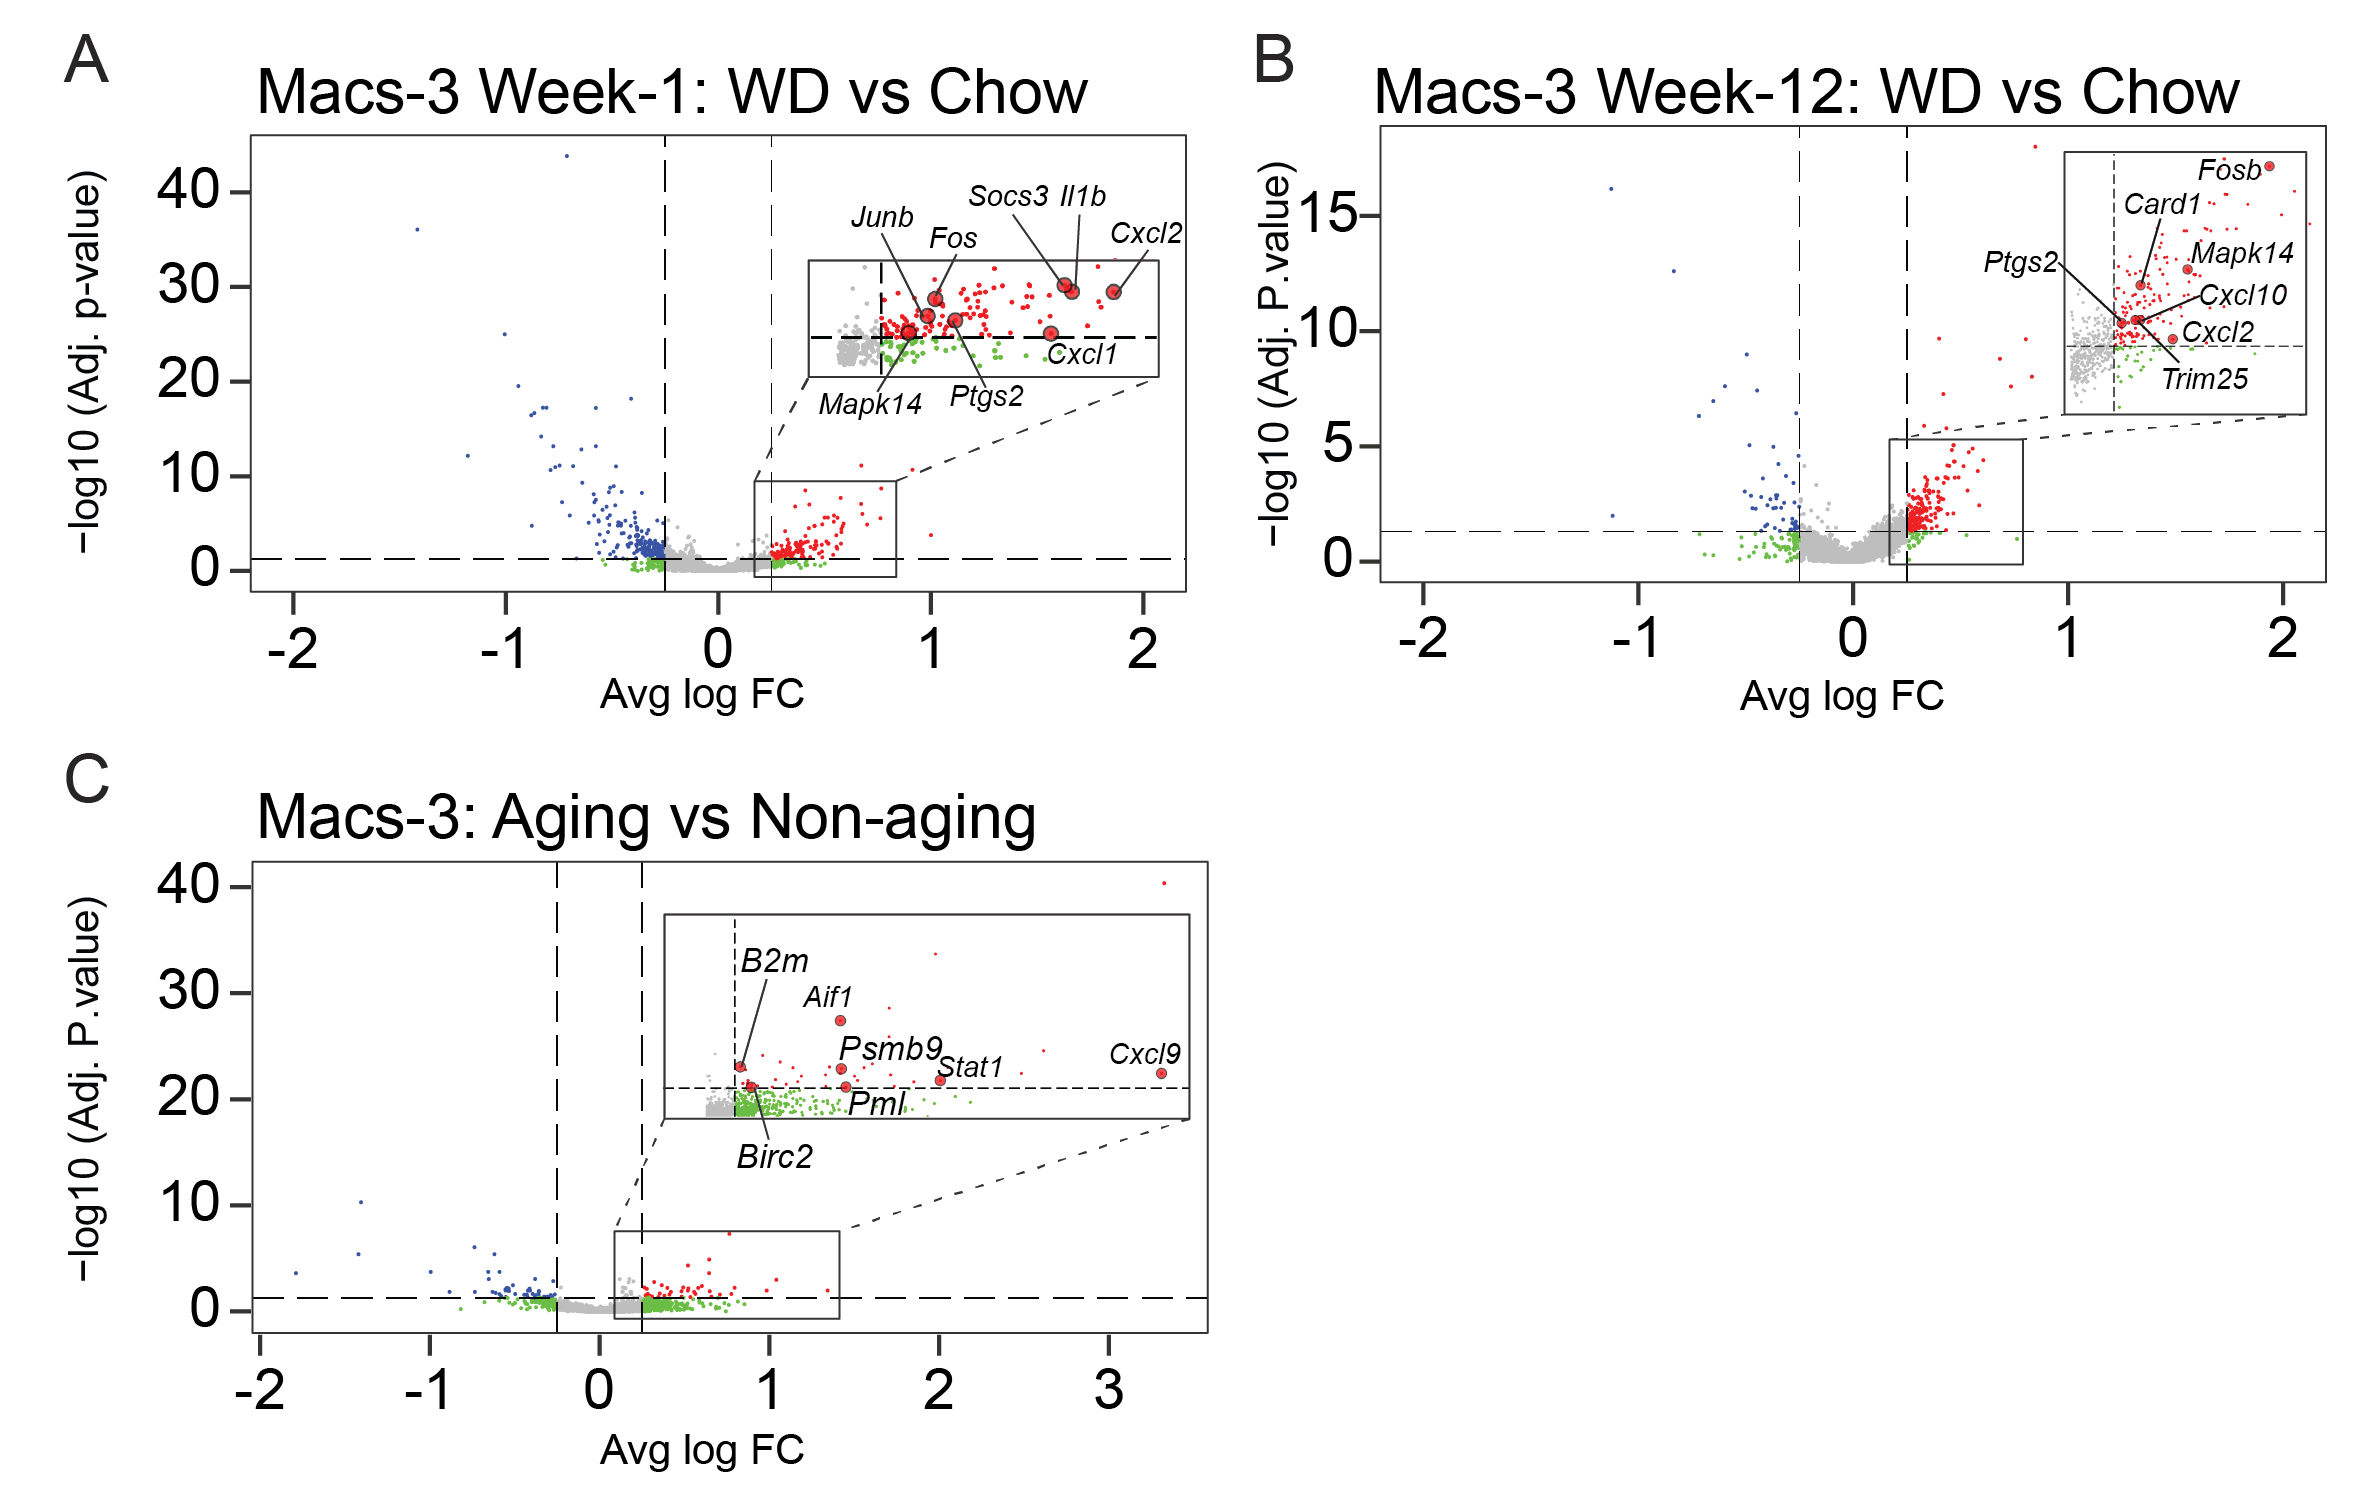
\includegraphics[width=\linewidth]{Chapter4/Fig/F2-11-01.png}
\caption[\glsentryshort{dge} analysis in Macs-3 macrophages]{\textbf{\gls{dge} analysis in Macs-3 macrophages.} \textbf{(A) - (C)} Volcano plots showing \gls{de} genes in Macs-3 sub-population, comparing \gls{wd} versus chow diet at Week-1 time-point \textbf{(A)}, \gls{wd} versus chow diet at Week-12 time-point \textbf{(B)} and chow diet-fed aging cohort versus chow diet-fed non-aging (W1 + W12) cohorts \textbf{(C)}.  The cells from different biological replicate cohorts were pooled together for the analysis. The dashed vertical lines represent $  \left|Avg. \log FC \right| $ = 0.25 and the dashed horizontal line represent $-\log_{10}(\num{0.05}) = 1.3$. Differentially up-regulated and down-regulated genes are depicted by red and blue dots respectively. Abbreviations: \gls{wd}, western diet; $Avg. \log\textsubscript{2} \glsentryshort{fc}$, $\log\textsubscript{2}$ \glsentrylong{fc} of the average expression of the gene between the two groups; Adj. p-value, adjusted p-value based on Bonferroni correction using all genes in the dataset.}
\label{fig:chp2_scrna_macrophages_macs3_dge}
\end{figure}

\par Consistent with the results from the \gls{dge} analysis \textbf{(\autoref{fig:chp2_scrna_macrophages_macs3_dge})}, Macs-3 did activate the type-1 \gls{ifn} response under both \gls{wd} and aging conditions. However, this response was notably intensified during aging (km-9). This heightened response is likely attributed to the enhanced canonical response and the absence of feedback inhibition by \textit{Stat3 / Socs3} \textbf{(\autoref{fig:chp2_scrna_macrophages_macs3_dge} A)}, which was observed in \gls{wd}. It might also be explained by the aging-specific attenuation of the \gls{perk} pathway (km-3), which has been proposed to maintain an immunosuppressive phenotype in macrophages \textbf{\cite{raines_perk_2022}}. Conversely, \gls{wd} feeding uniquely triggered the \gls{mtor} pathway (km-4) in Macs-3, further suggesting that it represents a non-canonical type-1 \gls{ifn} response \textbf{\cite{mazewski_type_2020}}. Furthermore, \gls{wd} feeding specifically triggered the activation of genes in the \gls{tnf}-$\alpha$ / \gls{nfkb} signaling pathway (km-6) in Macs-3, a change that was not evident during aging. This highlights the potential involvement of additional pro-inflammatory cytokines during metabolic stress as opposed to inflammaging.\\

\par Interestingly, despite Macs-2 exhibiting a lower activation profile compared to Macs-3, \gls{wd} feeding resulted in a stronger expression of genes coding for inflammatory cytokines and chemokines in Macs-2 \textbf{(\autoref{fig:app_scrna_macrophages_macs2_dge} A,B)}. In contrast, this induced up-regulation of cytokine genes observed in Macs-2 under \gls{wd} feeding conditions was not evident in the aging condition \textbf{(\autoref{fig:app_scrna_macrophages_macs2_dge} C)}. The Macs-2 macrophages also showed non-canonical type-1 \gls{ifn} responses, evident in the up-regulated \textit{Socs3} expression one week after starting the \gls{wd} feeding \textbf{(\autoref{fig:app_scrna_macrophages_macs2_dge} A)}. Intriguingly, the \gls{wd} triggered various inflammatory cytokine and chemokine gene expression, persisting twelve weeks into overnutrition \textbf{(\autoref{fig:app_scrna_macrophages_macs2_dge} B)}. In contrast, while Macs-2 in aging conditions exhibited signs of immune cell activation, it did not demonstrate cytokine expression \textbf{(\autoref{fig:app_scrna_macrophages_macs2_dge} C)}.\\


\begin{figure}[t]
\centering
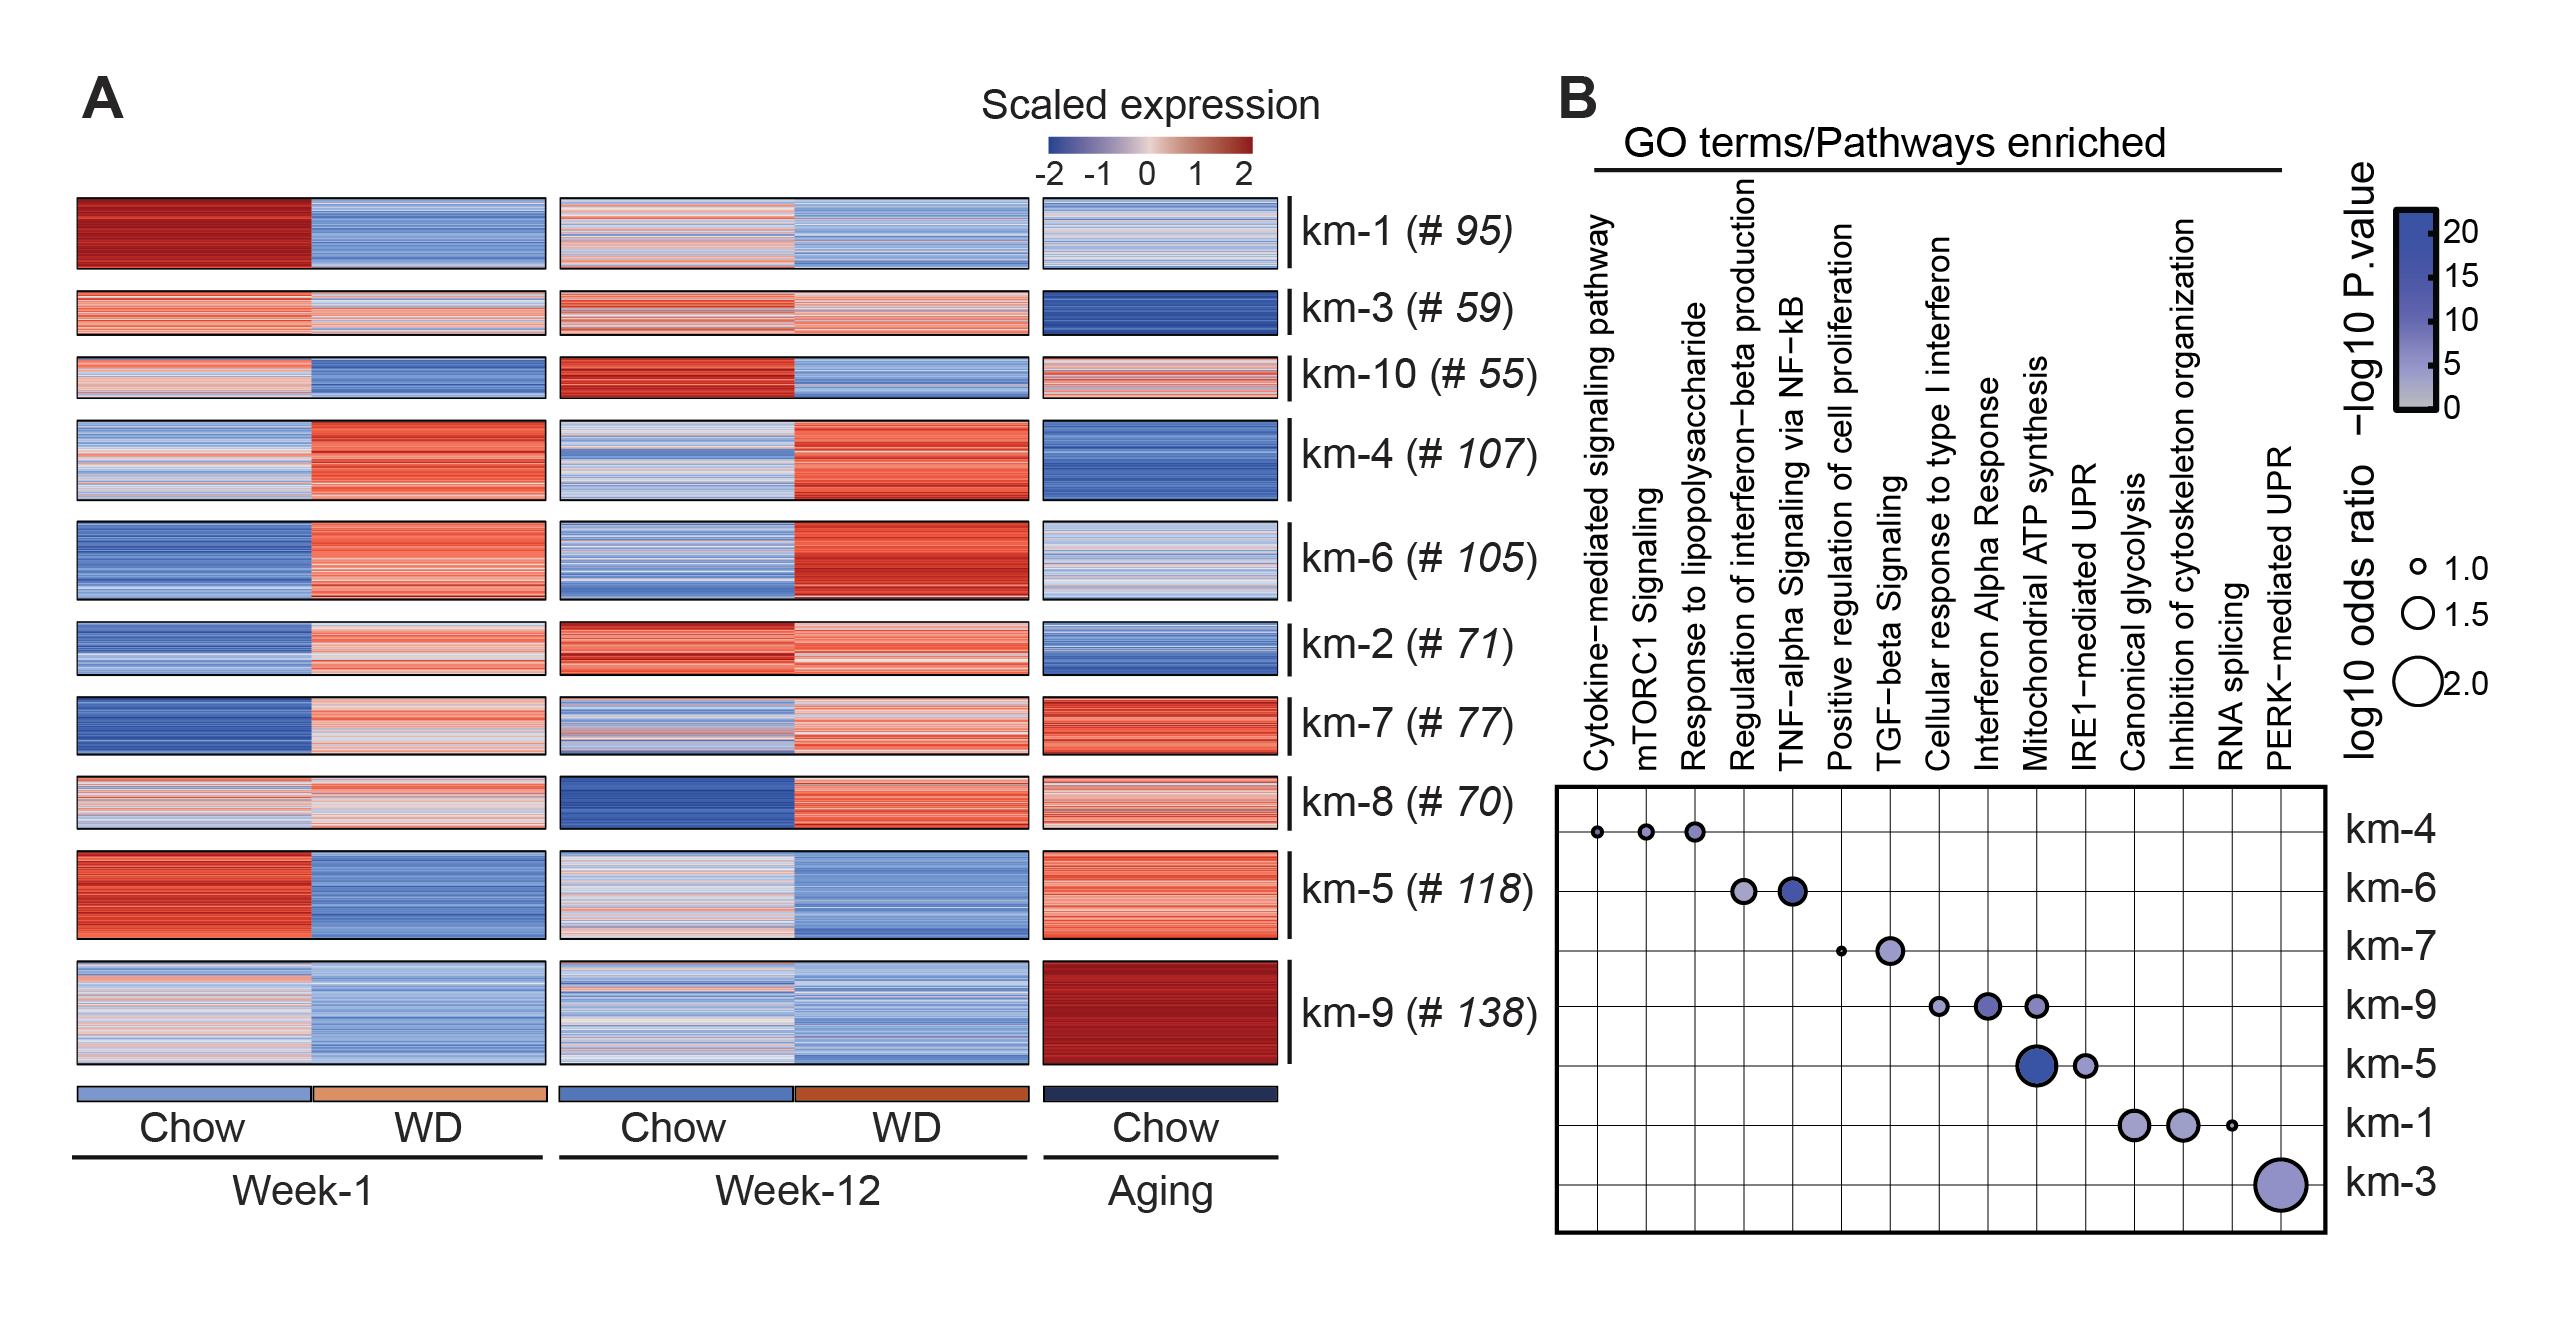
\includegraphics[width=\linewidth]{Chapter4/Fig/F2-11-02.png}
\caption[Expression patterns of \glsentryshort{de} genes in Macs-3 across overnutition and aging]{\textbf{Expression patterns of \gls{de} genes in Macs-3 across overnutition and aging.} \textbf{(A)} Heatmap depicting the scaled average expression of all 895 \gls{de} genes in Macs-3 sub-population across the experimental groups. The \gls{de} genes were clustered into 10 modules with \textit{k-means} clustering and are grouped by their modules in the heatmap. The number of genes in each \textit{k-means} module (km) is indicated in parentheses. \textbf{(B)} Dot plot depicting enriched \gls{go} terms or pathways in the selected modules from \textbf{(A)}. The color of the dots indicate the significance of the term in a particular module and the size of the dots correspond to odds ratio which measures the enrichment of overlapping genes between the modules and the annotated set relative to the expected random distribution.}
\label{fig:chp2_scrna_macrophages_macs3_clust}
\end{figure}

\par In summary, our analysis revealed an activation of the canonical type-1 \gls{ifn} response during inflammaging. While overnutrition can accelerate a similar process, it triggers a non-canonical signaling cascade thereby likely leading to a more pronounced inflammatory state.


\clearpage

\begin{comment}
    
\section[$\beta$-cells display distinct inflammatory profiles in response to obesity and aging]{$\beta$-cells display distinct inflammatory profiles in response\\to obesity and aging}
\label{sec:chp2_betacells}
Overnutrition and aging activate islet-associated macrophages, leading to varied inflammatory states in the islets. However, the response of pancreatic $\beta$-cells to these conditions, and how they might be affected by the altered inflammation, remains unclear. To explore this, we evaluated the metabolic phenotypes displayed by cohorts exposed to \gls{wd} and aging. Consistent with previous studies \textbf{\cite{}}, we noticed an acute islet dysfunction a week after initiating a \gls{wd} \textbf{(\autoref{fig:app_metab_betacells} A-D)}. Moreover, glucose intolerance and insulin resistance became noticeable after 12 weeks of overnutrition \textbf{(\autoref{fig:app_metab_betacells} E,F)}, coinciding with a compensatory rise in insulin secretion from the islets \textbf{(\autoref{fig:app_metab_betacells} G,H)}. Aging cohorts, however, retained normal glucose tolerance and insulin sensitivity \textbf{(\autoref{fig:app_metab_betacells} I,J)}, and their islets showed heightened insulin release under both basal and glucose-stimulated conditions in the \textit{in-vitro} culture \textbf{(\autoref{fig:app_metab_betacells} K,L)}.\\

%A critical facet of \gls{t2d} in $\beta$-cell dysfunction. However, the response of ... 
\par To characterize the islet $\beta$-cells, we further analyzed the $\beta$-cells derived from our \gls{scr} data. Following a sub-clustering analysis, we identified three $\beta$-cell sub-populations \textbf{(\autoref{fig:chp2_scrna_betacells1} A, \autoref{fig:app_scrna_betacells1} A)}. Compared to a previous single-cell analysis of 
murine islets \textbf{\cite{sachs_targeted_2020}} via label transfer \textbf{(\autoref{fig:app_scrna_betacells1} B)}, we observed that our $\beta$-3 sub-
population corresponded to the \textit{Cd81}\textsuperscript{+} immature $\beta$-cell sub-population \textbf{(\autoref{fig:app_scrna_betacells1} A, C)}. Whereas both $\beta$-1 and $\beta$-2 represented mature $\beta$-cells. $\beta$-1 exhibited enhanced \glslink{mtor}{mTORC1} signaling \textbf{(\autoref{fig:chp2_scrna_betacells1} B)} and $\beta$-2 displayed increased expression of genes involved in the peptide metabolic process \textbf{(\autoref{fig:chp2_scrna_betacells1} C)}. Unlike our observations in macrophages, the composition of the $\beta$-cell sub-populations remained highly stable under both \gls{wd} and aging conditions \textbf{(\autoref{fig:chp2_scrna_betacells1} E)}.\\

\begin{figure}[t!]
    \centering
    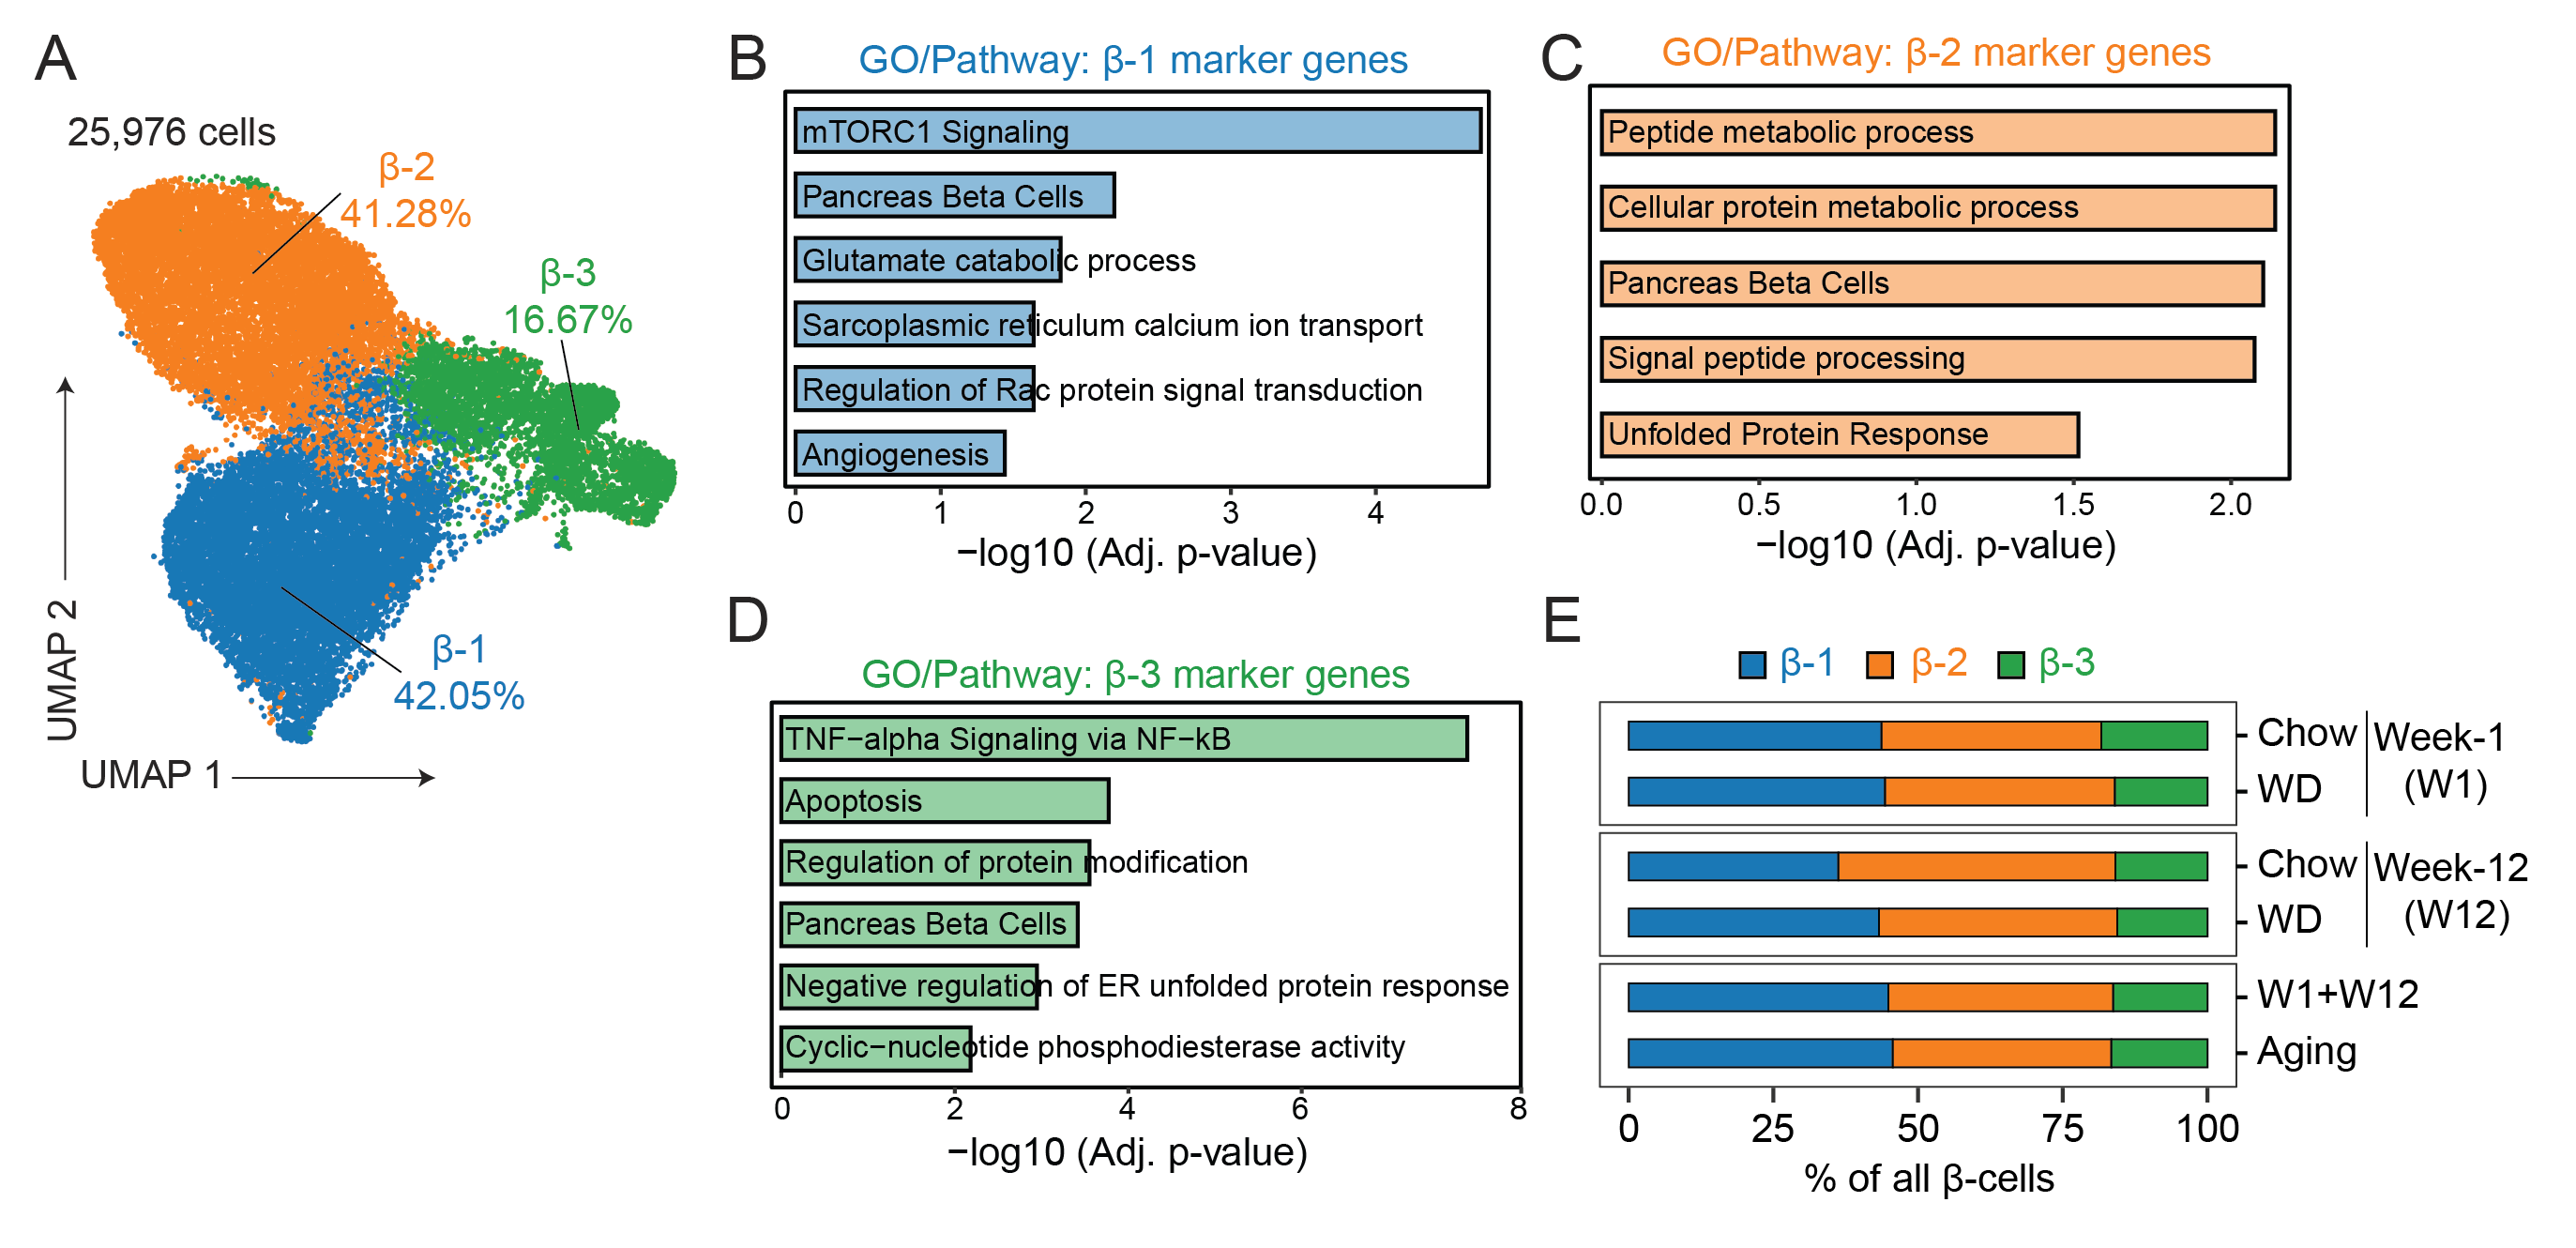
\includegraphics[width=\linewidth]{Chapter4/Fig/F2-12-02.png}
    \caption[Characterization of islet $\beta$-cells using \glslink{scr}{scRNA-seq}]{\textbf{Characterization of islet $\beta$-cells using \gls{scr}.} \textbf{(A)} \gls{umap} embedding of pancreatic islet $\beta$-cells, pooled from various experimental groups and replicates. Values indicate the overall proportion of each sub-population, defined based on marker gene expression. \textbf{(B-D)} Enriched \gls{go} terms among marker genes of $\beta$-1 \textbf{(B)}, $\beta$-2 \textbf{(C)} and $\beta$-3 \textbf{(D)}. Significance ($-\log_{10}$ adjusted p-value) of the enrichment are shown in bar plots. \textbf{(E)} The proportion of each $\beta$-cell sub-population in panel \textbf{(A)}, computed as a percentage of all $\beta$-cells in every experimental group. The cells from different biological replicate cohorts were pooled together.}
    \label{fig:chp2_scrna_betacells1}
\end{figure}
%\par Despite this, considerable changes in the transcriptome were observed across all β-cell sub-populations due to overnutrition and aging. 
\par To investigate the responses of islet $\beta$-cells to overnutrition and aging, we conducted a \gls{dge} analysis between \gls{wd} and chow diet fed cohorts after 1 and 12 weeks of feeding and between the chow diet fed aging cohort and the non-aging controls. Importantly, we observed that the three $\beta$-cell sub-populations responded similarly to \gls{wd} feeding and aging, as both, the direction and the magnitude of expression of the \gls{de} genes were similar across the three sub-populations \textbf{(\autoref{fig:app_scrna_betacells1} D-F)}. Based on these observations, we grouped all $\beta$-cells together, and re-performed the \gls{dge} analysis across all $\beta$-cells, identified 521 \gls{de} genes across all the experimental groups and clustered into gene modules \textbf{(\autoref{fig:chp2_scrna_betacells2} A)}. These modules encompass genes that display analogous expression patterns across overnutrition and aging conditions. Importantly, we identified modules that were unique to aging (km-9, km-10, and km-2), specific to \gls{wd} feeding (km-6, km-1, km-8, km-3, and km-7), or shared across both conditions (km-4 and km-5) \textbf{(\autoref{fig:chp2_scrna_betacells2} A)}. Through \gls{go} and pathway analysis \textbf{(\autoref{fig:chp2_scrna_betacells2} B)}, we found that overnutrition and aging typically boosted \glslink{oxphos}{OxPhos} (km-4), while concurrently weakening the expression of $\beta$-cell identity genes (km-5) \textbf{(\autoref{fig:chp2_scrna_betacells2} B)}. Changes exclusively linked to the \gls{wd} feeding involved a significant uptick in \gls{upr} (km-1, km-6 and km-8) and a distinct decline in genes linked to alternative splicing (km-3 and km-7) \textbf{(\autoref{fig:chp2_scrna_betacells2} B)}. Aging-related gene modules showed fewer enriched pathways likely due to fewer genes per module.\\ %We observed an aging-specific decrease in \textit{G6pc2} expression \textbf{(Fig. )} in β-cells, which is in line with their increased glucose sensitivity and enhanced insulin secretion at baseline glucose levels \textbf{(Fig. )}\\
\par Additionally, we identified genes activated by either acute (km-6) or chronic (km-8) \gls{wd} feeding. Specifically, the acute activation module (km-6), observed during 1 week of \gls{wd} feeding, was associated with \gls{tnf}-$\alpha$ pathway activation. Conversely, the chronic activation module (km-8), which was more evident after 12 weeks of \gls{wd} feeding, showed an up-regulation of genes linked to protein secretion. These findings indicate the a progression from islet dysfunction due to acute inflammatory response to compensatory insulin hypersecretion in response to prolonged metabolic stress  \textbf{(\autoref{fig:app_metab_betacells} D,H)}. Importantly, $\beta$-cells displayed a \gls{tnf}-$\alpha$ response after 1 week of \gls{wd} feeding, coinciding with an upsurge in \textit{Tnf} expression in Macs-2 in response to \gls{wd} feeding at the same time-point \textbf{(\autoref{fig:app_scrna_macrophages_macs2_dge} A)}.\\

\begin{figure}[t!]
    \centering
    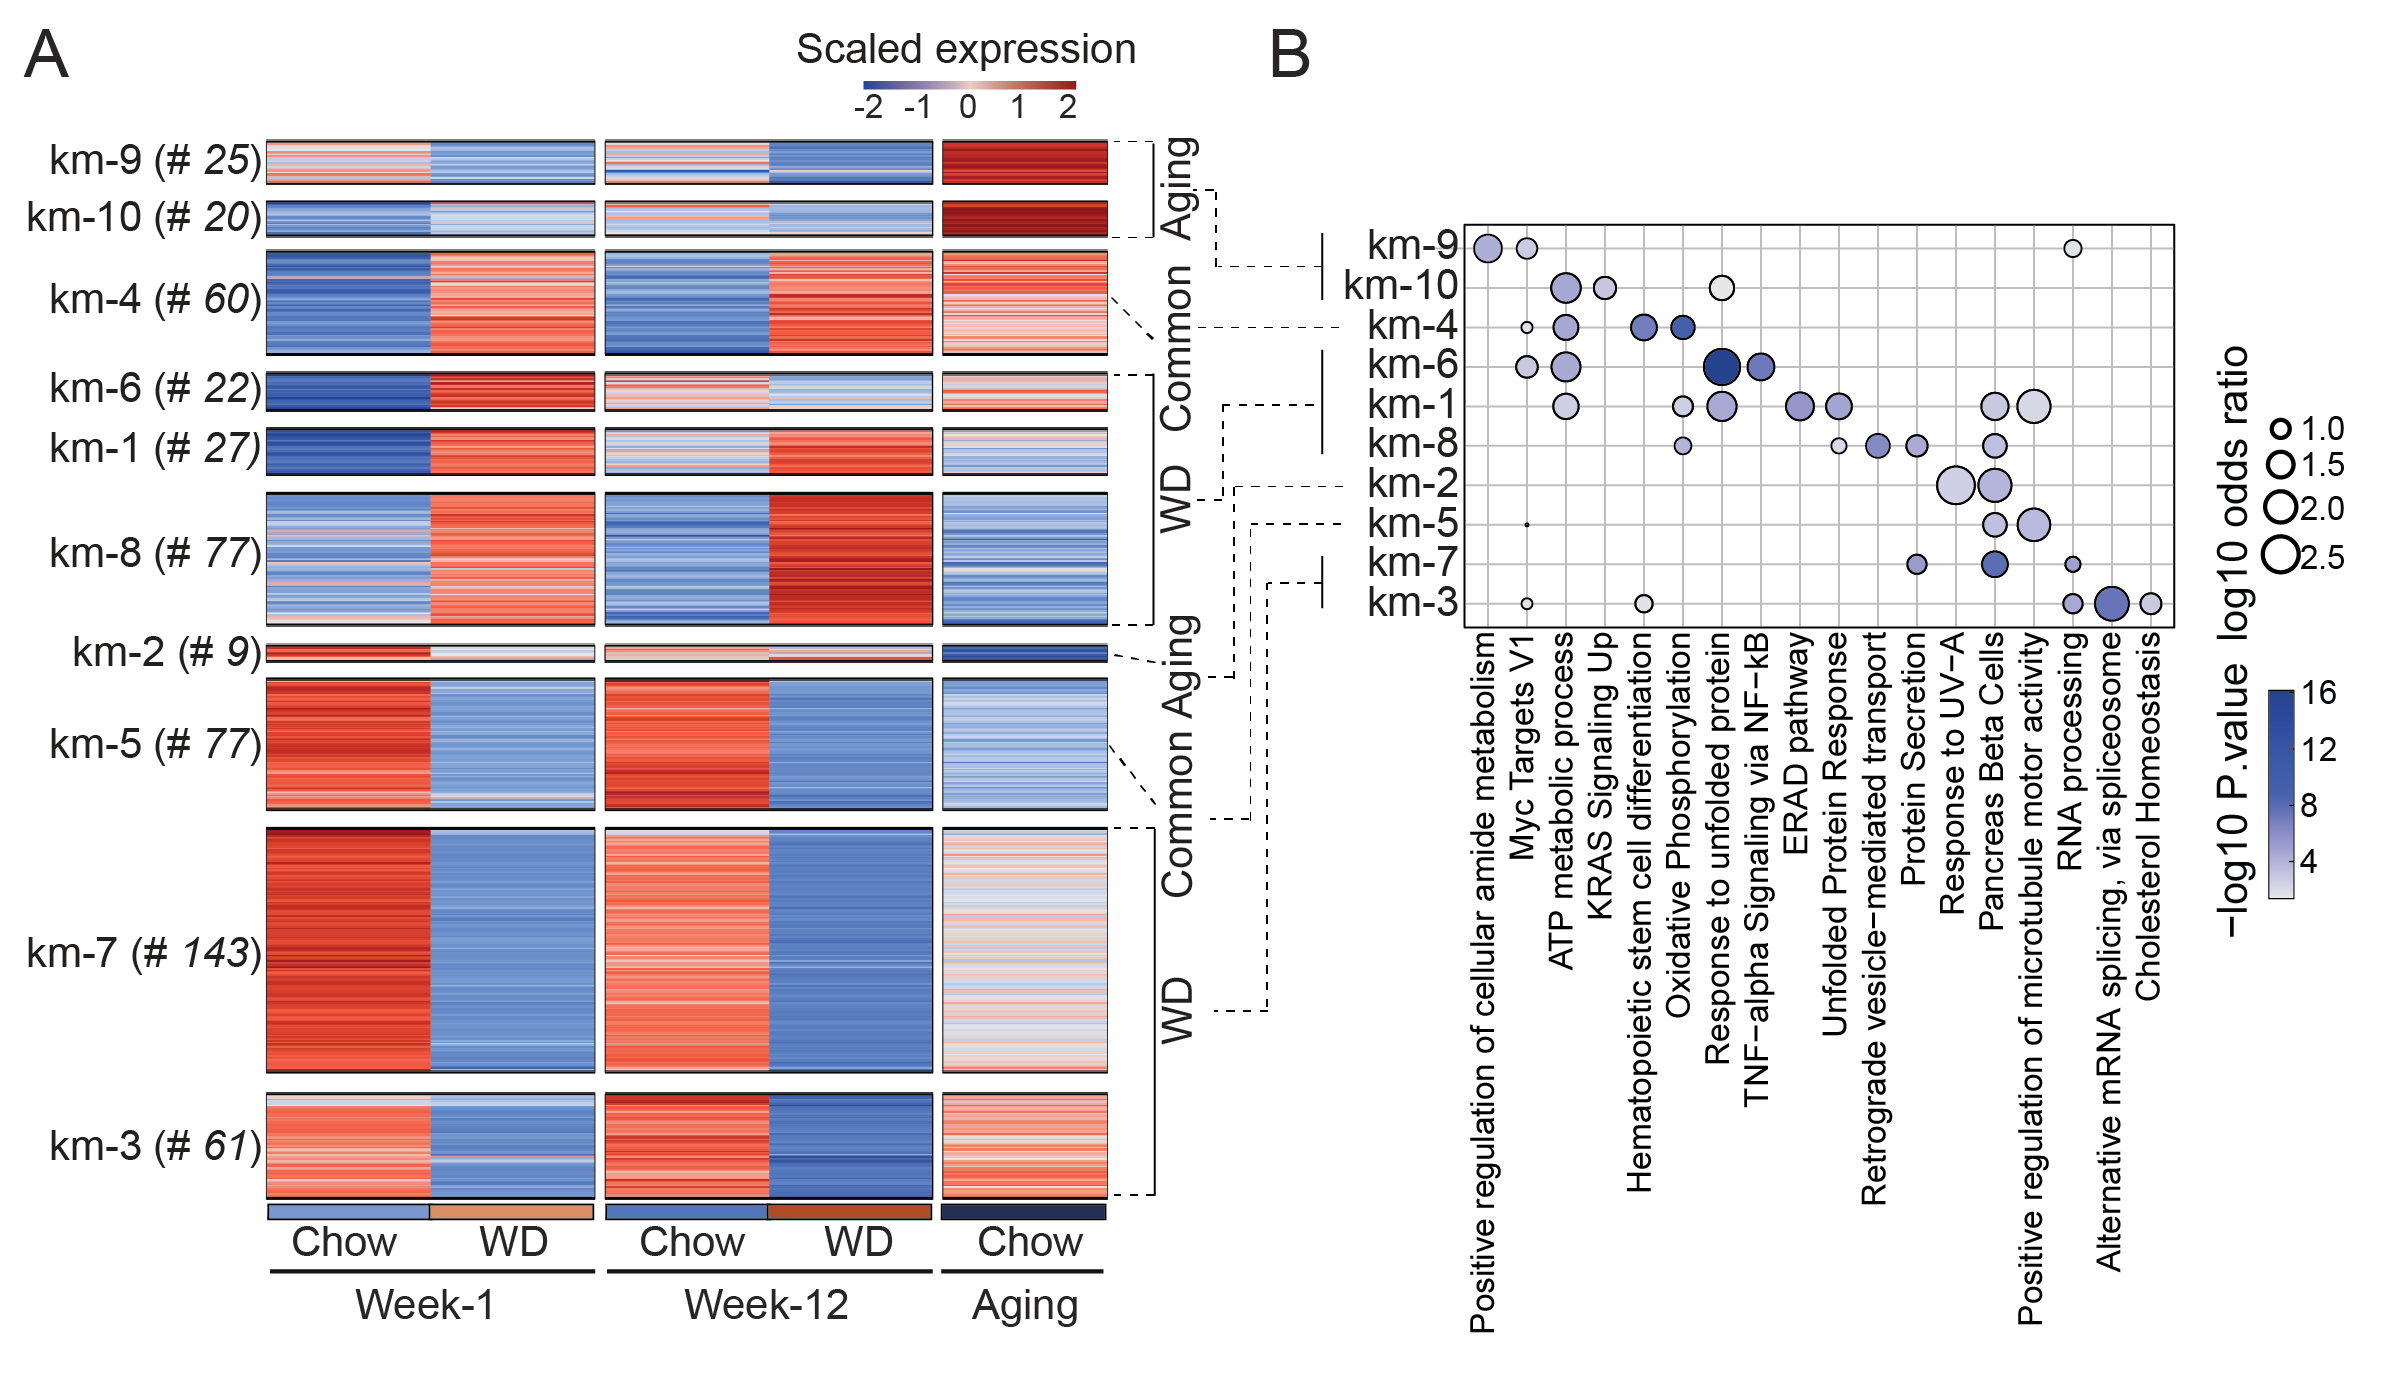
\includegraphics[width=\linewidth]{Chapter4/Fig/F2-12-01.png}
    \caption[\glslink{dge}{DGE} analayis in $\beta$-cells across \glslink{wd}{WD} feeding and aging]{\textbf{\gls{dge} analysis in $\beta$-cells across \gls{wd} feeding and aging.} \textbf{(A)} Heatmap depicting the scaled average expression of all \gls{de} genes in $\beta$-cells across the experimental groups (columns). The \gls{de} genes were clustered into 10 modules with the k-means clustering and are grouped by their modules in the heatmap (rows). \textbf{(B)} Dot plot depicting enriched \gls{go} terms or pathways in the selected modules from panel \textbf{(A)}. The color of the dots indicate the significance of the term in a particular module and the size of the dots correspond to odds ratio which measures the enrichment of overlapping genes between the modules and the annotated set relative to the expected random distribution. }
    \label{fig:chp2_scrna_betacells2}
\end{figure}

\par In conclusion, our analysis delineated the molecular responses of $\beta$-cells to \gls{wd} and aging established a possible link between $\beta$-cell transcriptomic profiles and the inflammatory environment dictated by islet-associated macrophages, offering insights into changes in $\beta$-cell function in response to overnutition and aging.

%\clearpage

\end{comment}

%\clearpage

\section[Metabolic stress accelerates aging-induced accumulation of CD8\textsuperscript{+} cytotoxic T-cells in the pancreas]{Metabolic stress accelerates aging-induced accumulation\\of CD8\textsuperscript{+} cytotoxic T-cells in the pancreas}
\label{sec:sc_tcells}

While there has been considerable focus on the role of islet macrophages during obesity-induced islet inflammation, research on adaptive immune components, particularly T-cells is less common due to their low numbers within the islets, thereby making their detailed characterization more challenging. The immune cell focused \gls{imc} panel \textbf{(\autoref{tab:app_imc_panel})} allowed us to characterize the T-cell populations in the pancreatic tissue in great detail. Our \gls{imc} analysis revealed an increase in pancreatic T-cells during both overnutrition and aging conditions \textbf{(\autoref{fig:chp2_imc_tcells1} A)}. In particular, we observed an expansion of CD8\textsuperscript{+} activated effector-like T-cells in the pancreas, which was more pronounced under \gls{wd} feeding \textbf{(\autoref{fig:chp2_imc_tcells1} B,D)}. However, similar to the previously observed variability in the F4/80\textsuperscript{\textit{low}} macrophage population \textbf{(\autoref{fig:chp2_imc_macrophages2} A,} middle\textbf{)}, the 


\begin{figure}[b!]
\centering
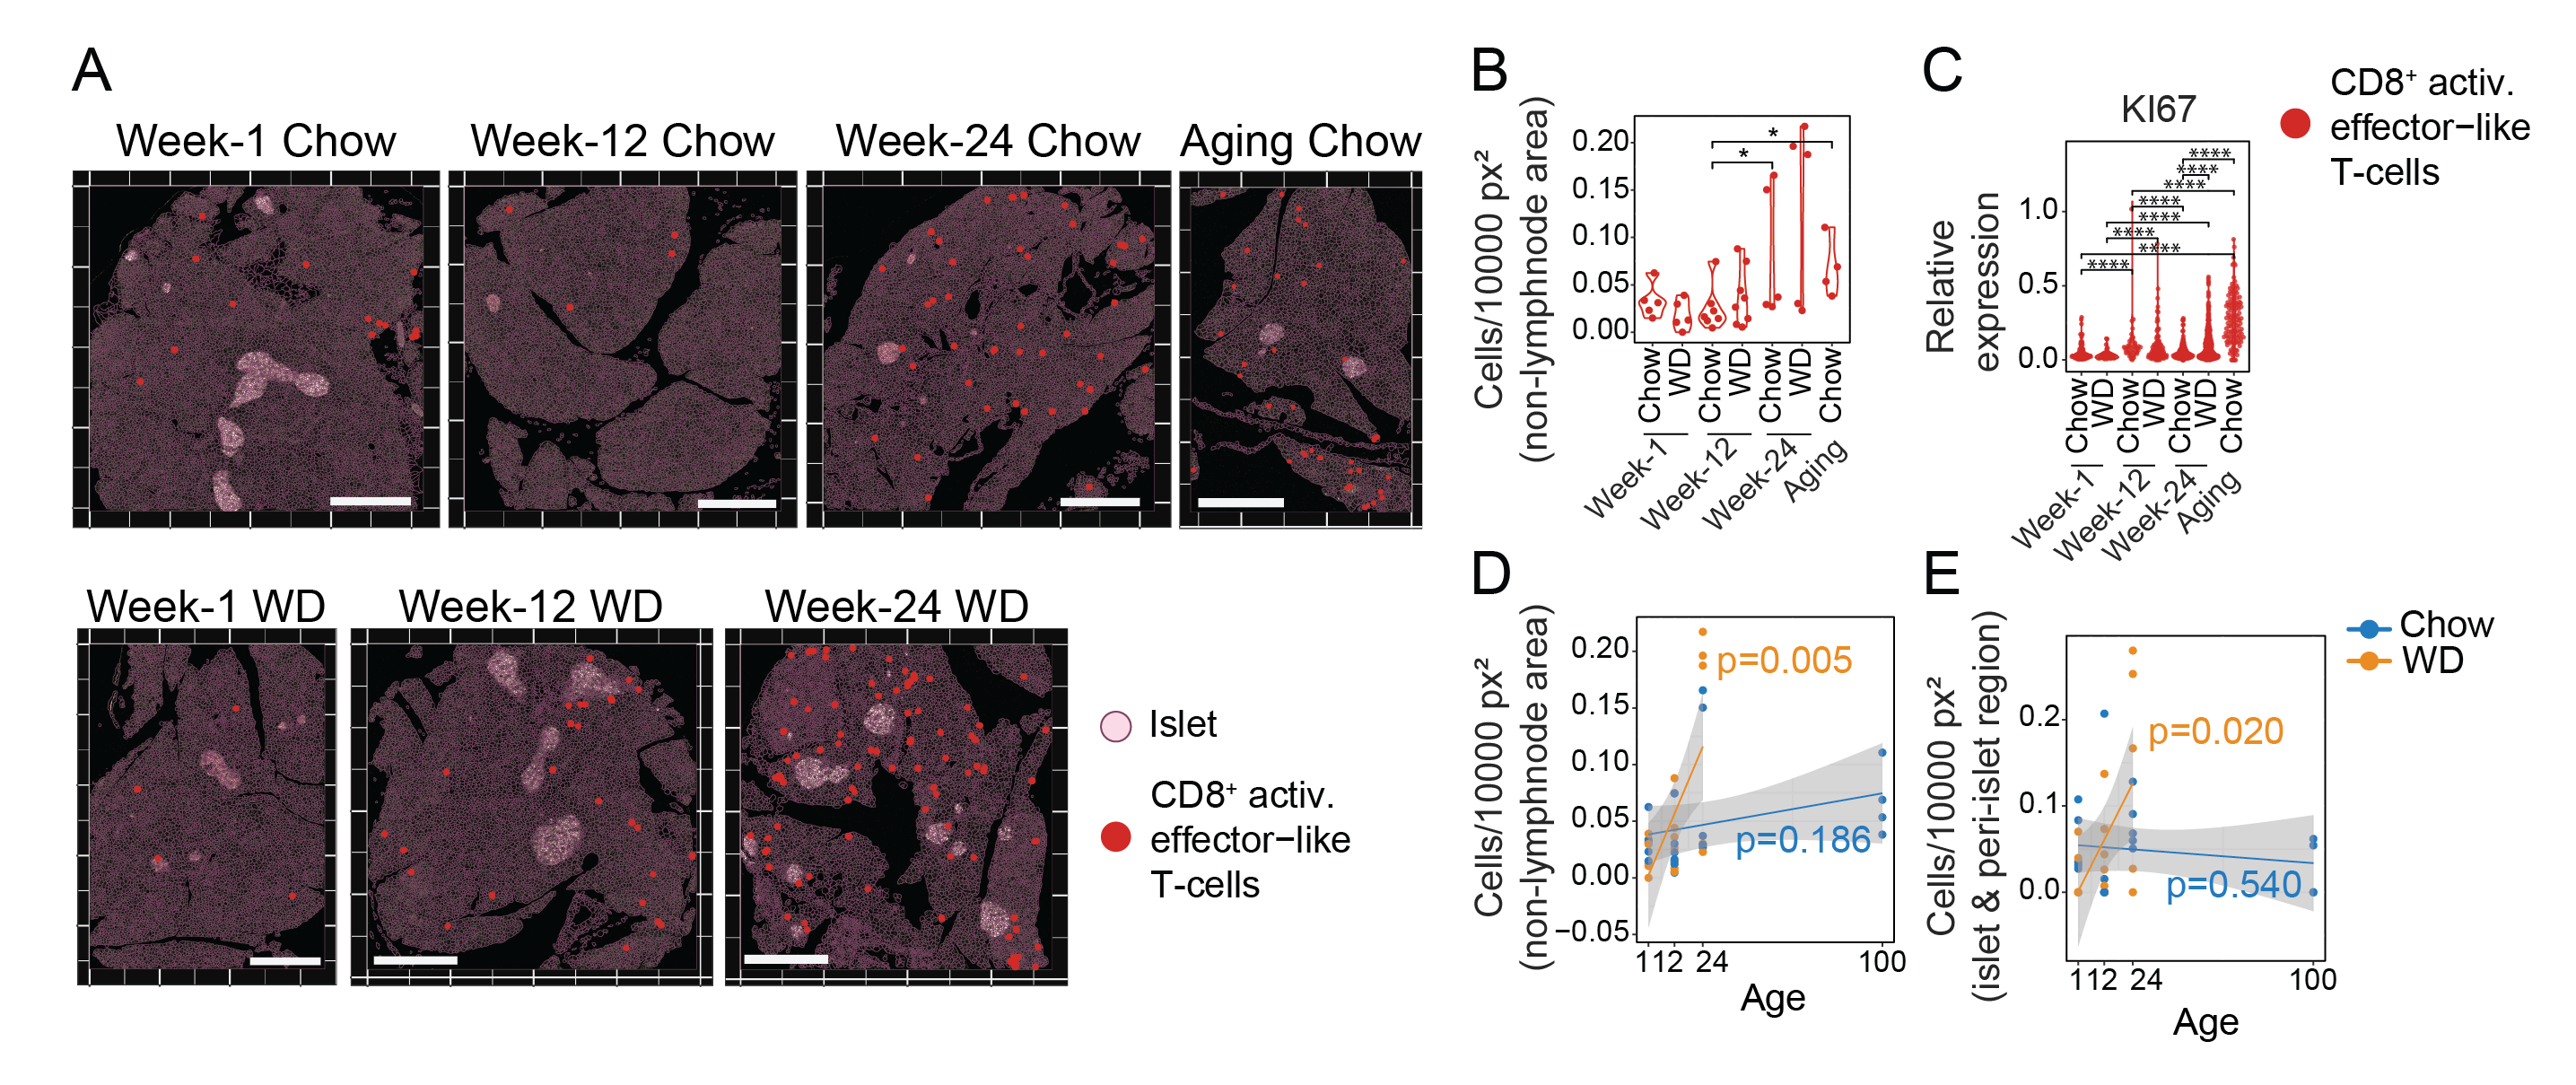
\includegraphics[width=\linewidth]{Chapter4/Fig/F2-10-02.png}
\caption[Accelerated accumulation of CD8\textsuperscript{+} cytotoxic T-cells in pancreas]{\textbf{Accelerated accumulation of CD8\textsuperscript{+} cytotoxic T-cells in pancreas in response to \gls{wd} feeeding.} \textbf{(A)} Representative \glspl{roi} showing CD8\textsuperscript{+} activated effector-like T-cells in the pancreas. Pancreatic islet regions are marked by raw INS signal (white).  Scale bar 500 \textmu m. \textbf{(B)} Violin plot displaying the densities of CD8\textsuperscript{+} activated effector-like T-cells in non-lymph node pancreatic regions, presented for each mouse across the different experimental conditions. \textbf{(C)} Violin plot depicting \textit{arcsinh} transformed KI67 channel expression of CD8\textsuperscript{+} activated effector-like T cells across experimental groups. \textbf{(D) - (E)} Scatter plot depicting the density of CD8\textsuperscript{+} activated effector-like T-cells in the pancreas \textbf{(D)} and in the pancreatic islet and peri-islet regions \textbf{(E)} across experimental groups. Linear regression fits representing the cell density trends over time are plotted as solid lines. The 95\% confidence intervals for each linear regression are highlighted in grey. $\textsuperscript{*} p < 0.05, \textsuperscript{**} p < 0.01, \textsuperscript{***} p < 0.001, \textsuperscript{***} p < 0.0001$. P-values were calculated using the Wilcoxon rank-sum test with Bonferroni correction. \textit{This data and figure were originally generated by Dr. Matthias Barone and reused here with permission.}}
\label{fig:chp2_imc_tcells1}
\end{figure}

\clearpage

\gls{wd} feeding also resulted in high variability in the dynamics of this T-cell population. In line with these observations, we found elevated levels of KI67 channel expression within these T-cells under both overnutrition and aging conditions \textbf{(\autoref{fig:chp2_imc_tcells1} C)}. This led us to question whether these CD8\textsuperscript{+} activated effector-like T-cells are further recruited to the pancreatic islets under metabolic and age-induced stress. To investigate this, we analyzed the cell density within the islets and their peripheral regions. We observed significant enrichment of CD8\textsuperscript{+} activated effector-like T-cells in the peri-islet regions under \gls{wd} conditions, but not during aging \textbf{(\autoref{fig:chp2_imc_tcells1} E)}.\\

%\clearpage

\par The CD45 enrichment approach allowed us to recover a considerable proportion of T-cells from within the pancreatic islets. To gain deeper insights into the dynamics of T-cell sub-populations within the pancreatic islets, we conducted a sub-clustering analysis of our single-cell data, including the total cellular space of non-B-cell lymphocytes \textbf{(}see \hyperref[subsubsec:met_chp2_immuneendo]{\textbf{Methods}}\textbf{)}. We identified several different T-cell sub-populations, together with other lymphocytes such as \glspl{ilc} -  \gls{ilc}2 and \gls{ilc}3 and \gls{nk} cells \textbf{(\autoref{fig:chp2_scrna_tcells1} A,C; \autoref{fig:app_scrna_tcells1} C,D)}. %It is noteworthy that the major T-cell sub-populations identified within the pancreatic islets from single-cell data mirrored those observed in the whole pancreas from \gls{imc} analysis.  
Based on marker expression, we identified  CD8\textsuperscript{+} cytotoxic T-cells, CD8\textsuperscript{+} memory T-cells, and \gls{treg} within the islets \textbf{(\autoref{fig:app_scrna_tcells1})}. These subsets exhibited a strong phenotypic alignment with the CD8\textsuperscript{+} activated effector-like T-cells, CD4\textsuperscript{+} / CD8\textsuperscript{+} memory-like cells, and \gls{treg} defined in our \gls{imc} data respectively \textbf{(\autoref{fig:app_scrna_tcells1} A,B)}. The precise correlation was underscored by their characteristic expression of EOMES (\textit{Eomes}), CD127 (\textit{Il7r}) and FOXP3 (\textit{Foxp3}), respectively \textbf{(\autoref{fig:app_scrna_tcells1} A,B)}. The whole transcriptome analysis revealed additional marker genes in the CD8\textsuperscript{+} cytotoxic T-cells, such \textit{Gzmk} (granzyme) and \textit{Ccl5} \textbf{(\autoref{fig:chp2_scrna_tcells1} C)}. Interestingly, similar to the CD8\textsuperscript{+} activated effector-like T-cells seen in the \gls{imc} data, the islet-associated CD8\textsuperscript{+} cytotoxic T-cells identified in the \gls{scr} data also expanded in response to \gls{wd} feeding \textbf{(\autoref{fig:chp2_scrna_tcells1} B)}. Moreover,this expansion was significant during aging within the islets in the \gls{scr} data \textbf{(\autoref{fig:chp2_scrna_tcells1} B)} compared to previous \gls{imc} analyses \textbf{(\autoref{fig:chp2_imc_tcells1} E)}.\\

\par Additionally, our \gls{scr} analysis provided increased resolution in identifying T-cell sub-populations within pancreatic islets, distinguishing two distinct sub-populations of naive T-cells marked by CD4 and CD8 \textbf{(\autoref{fig:chp2_scrna_tcells1} A,C; \autoref{fig:app_scrna_tcells1} C)}. These correspond to a single CD4\textsuperscript{+}/CD8\textsuperscript{+} non-proliferative, silent T-cell sub-population in our \gls{imc} data, characterized by high CD127 and low KI67 protein expression \textbf{(\autoref{fig:app_scrna_tcells1} A)}. We further revealed additional rare T-cell sub-populations within the islet, including Th1-like, Tfh-like, Naive-translation T-cells, \gls{ifn}-responsive T-cells, and a subset of $\gamma\delta$ T-cells \textbf{(\autoref{fig:chp2_scrna_tcells1} A,C; \autoref{fig:app_scrna_tcells1} C,D)}.\\


% The whole transcriptomic analysis further augmented our resolution in detecting islet-associated T-cell sub-populations. Notably, we identified two distinct naive T-cell sub-populations, each manifesting differential CD4 and CD8 expression profiles \textbf{(\autoref{fig:chp2_scrna_tcells1} A,C; \autoref{fig:app_scrna_tcells1} C)}. This observation correlates with the mixed CD4\textsuperscript{+}/CD8\textsuperscript{+} non-proliferative silent T-cell cluster defined in our \gls{imc} data, which was also characterised by high CD127 but low KI67 protein expression (\textbf{Supp. Fig.\ref{FIG} A}). Both, the \gls{scr} and \gls{imc} analyses (\textbf{Fig.\ref{fig2-10} H} and \textbf{Supp. Fig.\ref{FIG} A}) revealed highest EOMES/\textit{Eomes} expression for the CD8\textsuperscript{+} cytotoxic / activated effector-like T-cells. The cytotoxic T-cell subpopulation in the single-cell data was also characterized by high expression of granzyme K (\textit{Gzmk}) and chemokine ligand 5 \textit{Ccl5} (\textbf{Fig.\ref{fig2-10} H}).

\begin{figure}[t!]
\centering
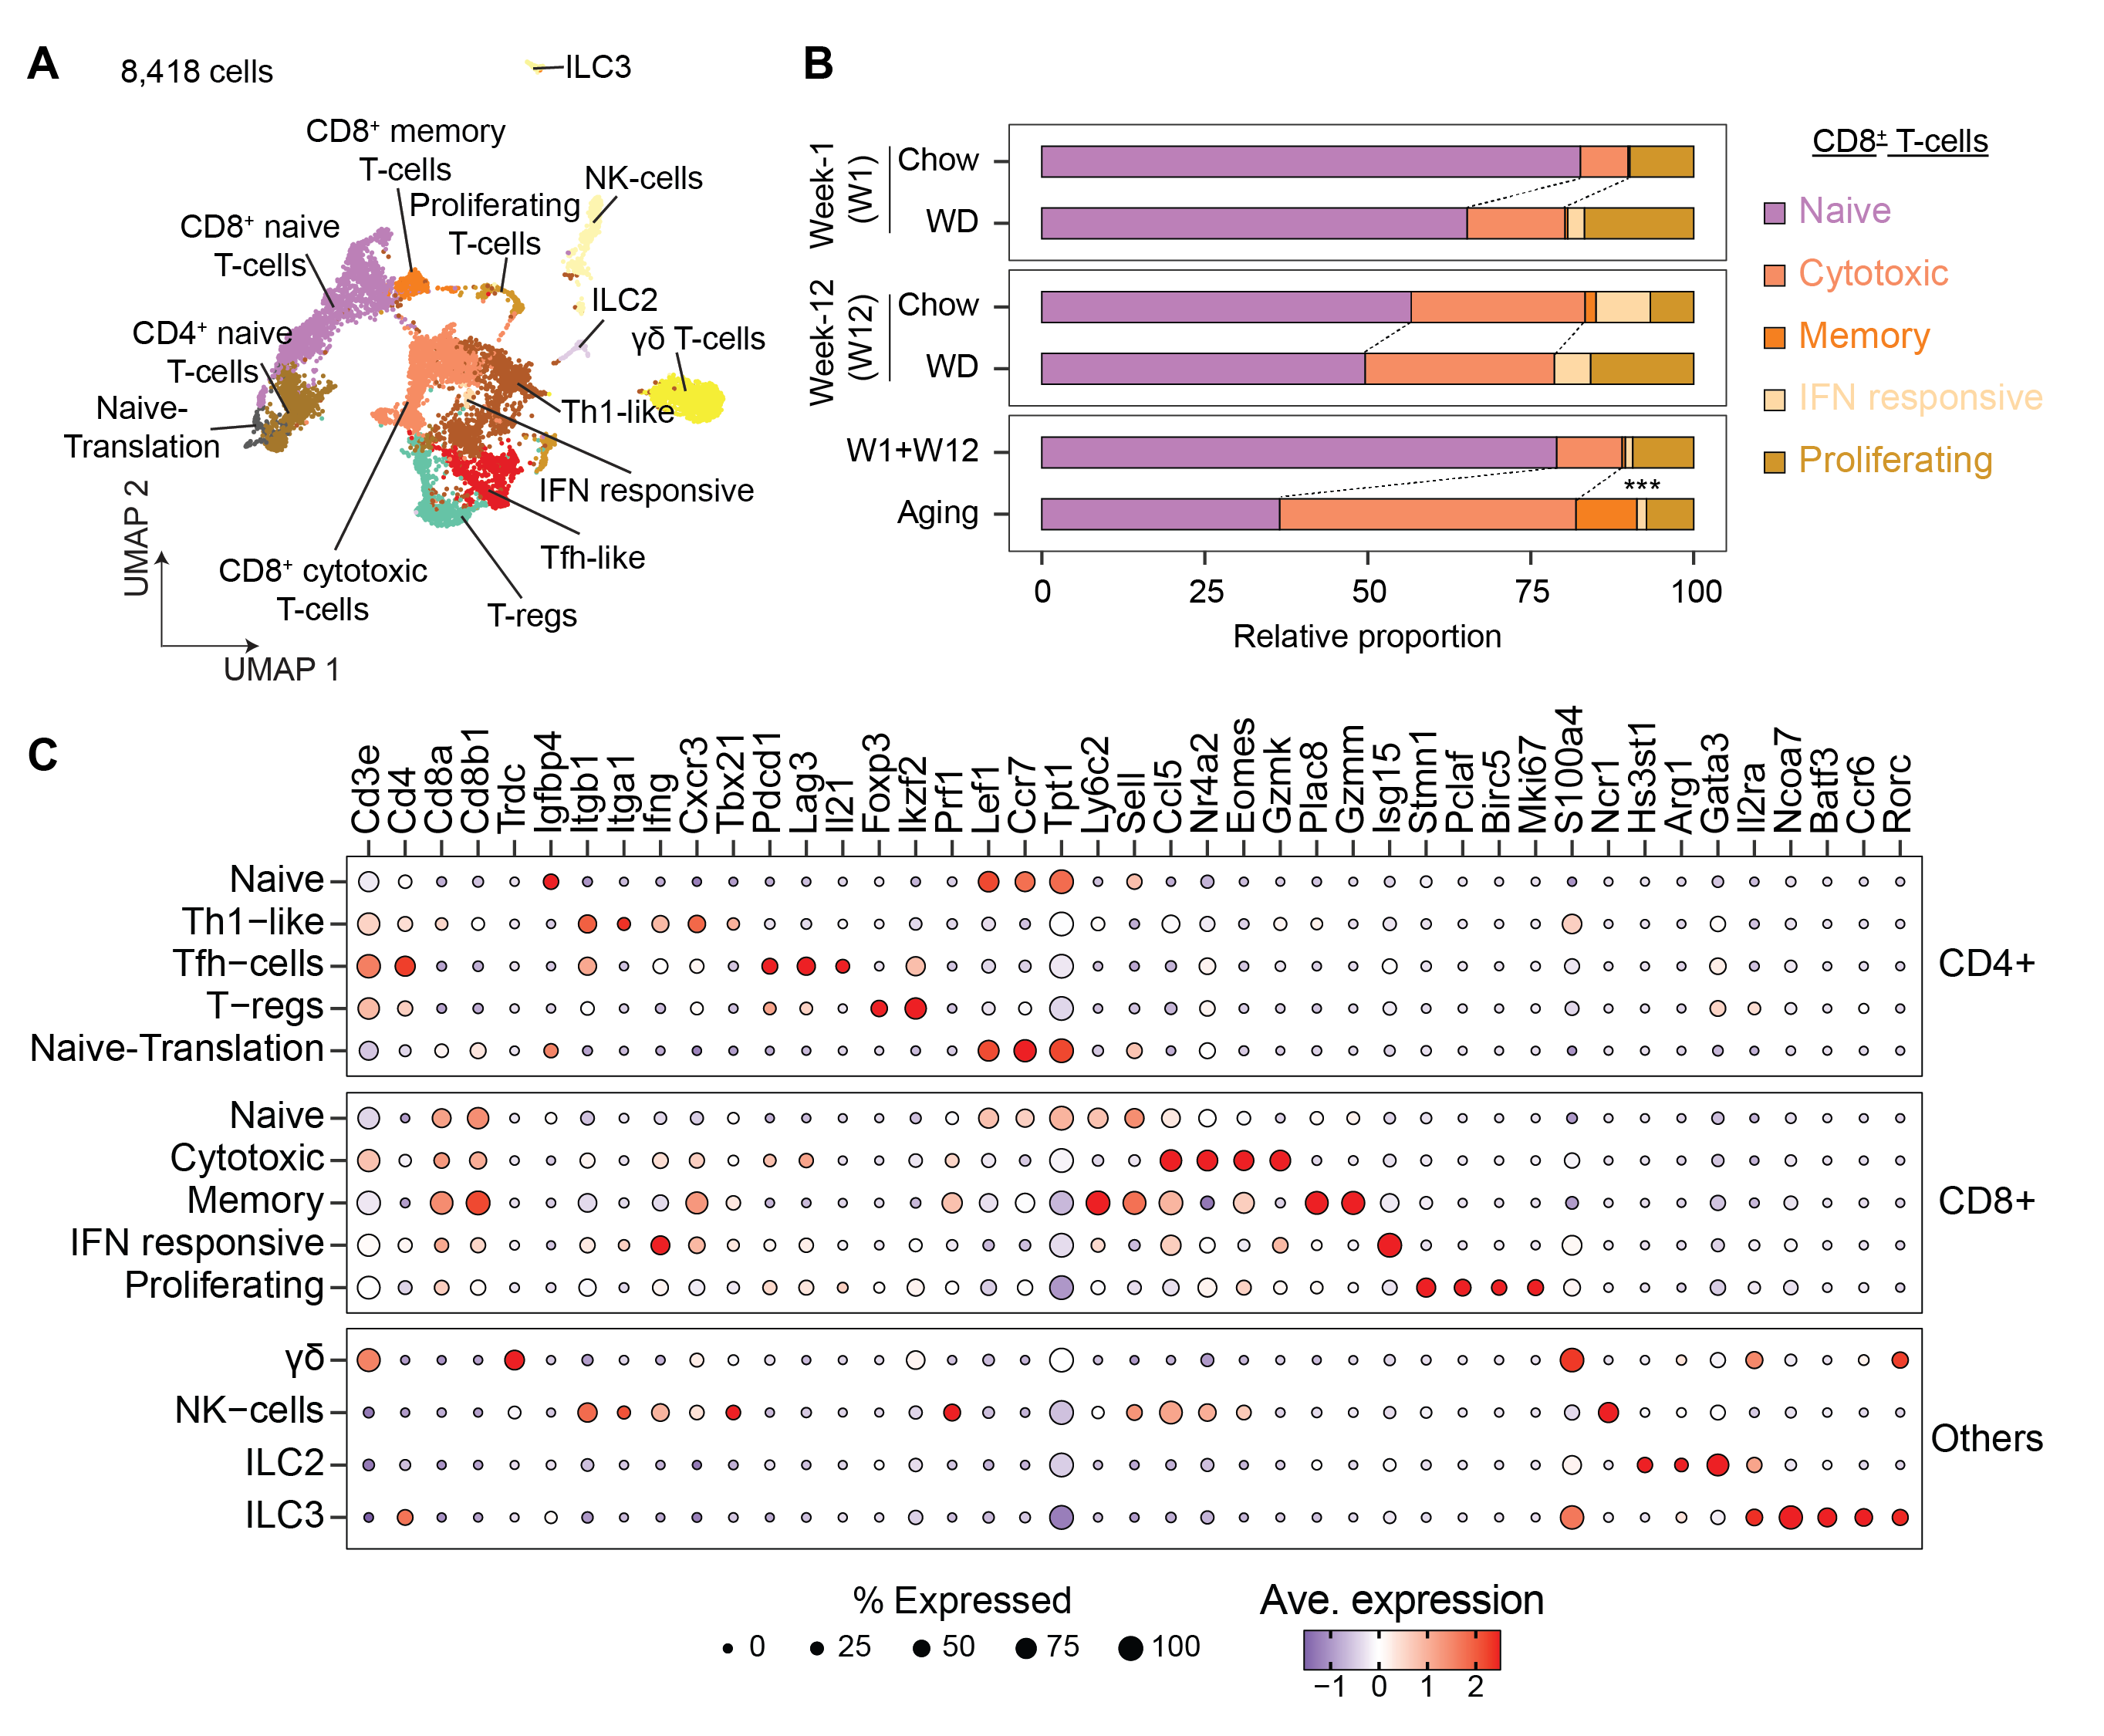
\includegraphics[width=\linewidth]{Chapter4/Fig/F2-10-01.png}
\caption[Characterization of T-cell sub-populations in \glsentryshort{scr} data]{\textbf{Characterization of islet-associated T-cell sub-populations in \gls{scr} data.} \textbf{(A)} \gls{umap} embedding of islet-associated T- and other lymphocyte sub-populations pooled across all experimental groups. Cell types were defined based on marker gene expression. \textbf{(B)} The proportion of each CD8\textsuperscript{+} T-cell sub-population in \textbf{(A)}, computed as a percentage of all CD8\textsuperscript{+} cells in every experimental group. The cells from different biological replicate cohorts were pooled together.  $\textsuperscript{*} p < 0.05, \textsuperscript{**} p < 0.01, \textsuperscript{***} p < 0.001$. p-values were calculated from a mixed-effects binomial model. \textbf{(C)} Dot plot depicting hallmark genes for all annotated T- and other lymphocyte sub-populations in \textbf{(A)}. The color of the dots represent the scaled average expression of the genes and the size of the dots correspond to the percentage of cells expressing the gene.
}
\label{fig:chp2_scrna_tcells1}
\end{figure}

\par Collectively, combining \gls{imc} and single-cell analysis, we have provided a comprehensive portrayal of T-cells within the pancreas, elucidating their population dynamics in both the exocrine and endocrine compartments under overnutrition and aging conditions. Key observations included an aging-induced expansion of \textit{Eomes} expressing CD8\textsuperscript{+} cytotoxic T-cells, both in the pancreas and the islets, which was accelerated by metabolic stress.

%\clearpage

\section[CD8\textsuperscript{+} cytotoxic T-cells receive signals from \glsentryshort{ifn}-activated macrophages]{CD8\textsuperscript{+} cytotoxic T-cells receive signals from \gls{ifn}-activated\\macrophages}
\label{sec:chp2_cell_cell}

Under metabolic stress, we observed a metabolic stress-induced enhanced accumulation of type-1 \gls{ifn} responsive inflammatory macrophages within the islets in our \gls{scr} data \textbf{(\autoref{fig:chp2_scrna_macrophages} D)} and CD8\textsuperscript{+} activated-effector like T-cells in the peri-islet regions \textbf{(\autoref{fig:chp2_imc_tcells1} E)}. As activated macrophages can elicit T-cell stimulatory signals, we investigated their inter-cellular communication potential by performing \gls{lri} analysis (see \hyperref[subsubsec:met_chp2_cellcell]{\textbf{Methods}}).

\subsubsection{\large Intercellular interactions under acute overnutrition}


\begin{figure}[b!]
\centering
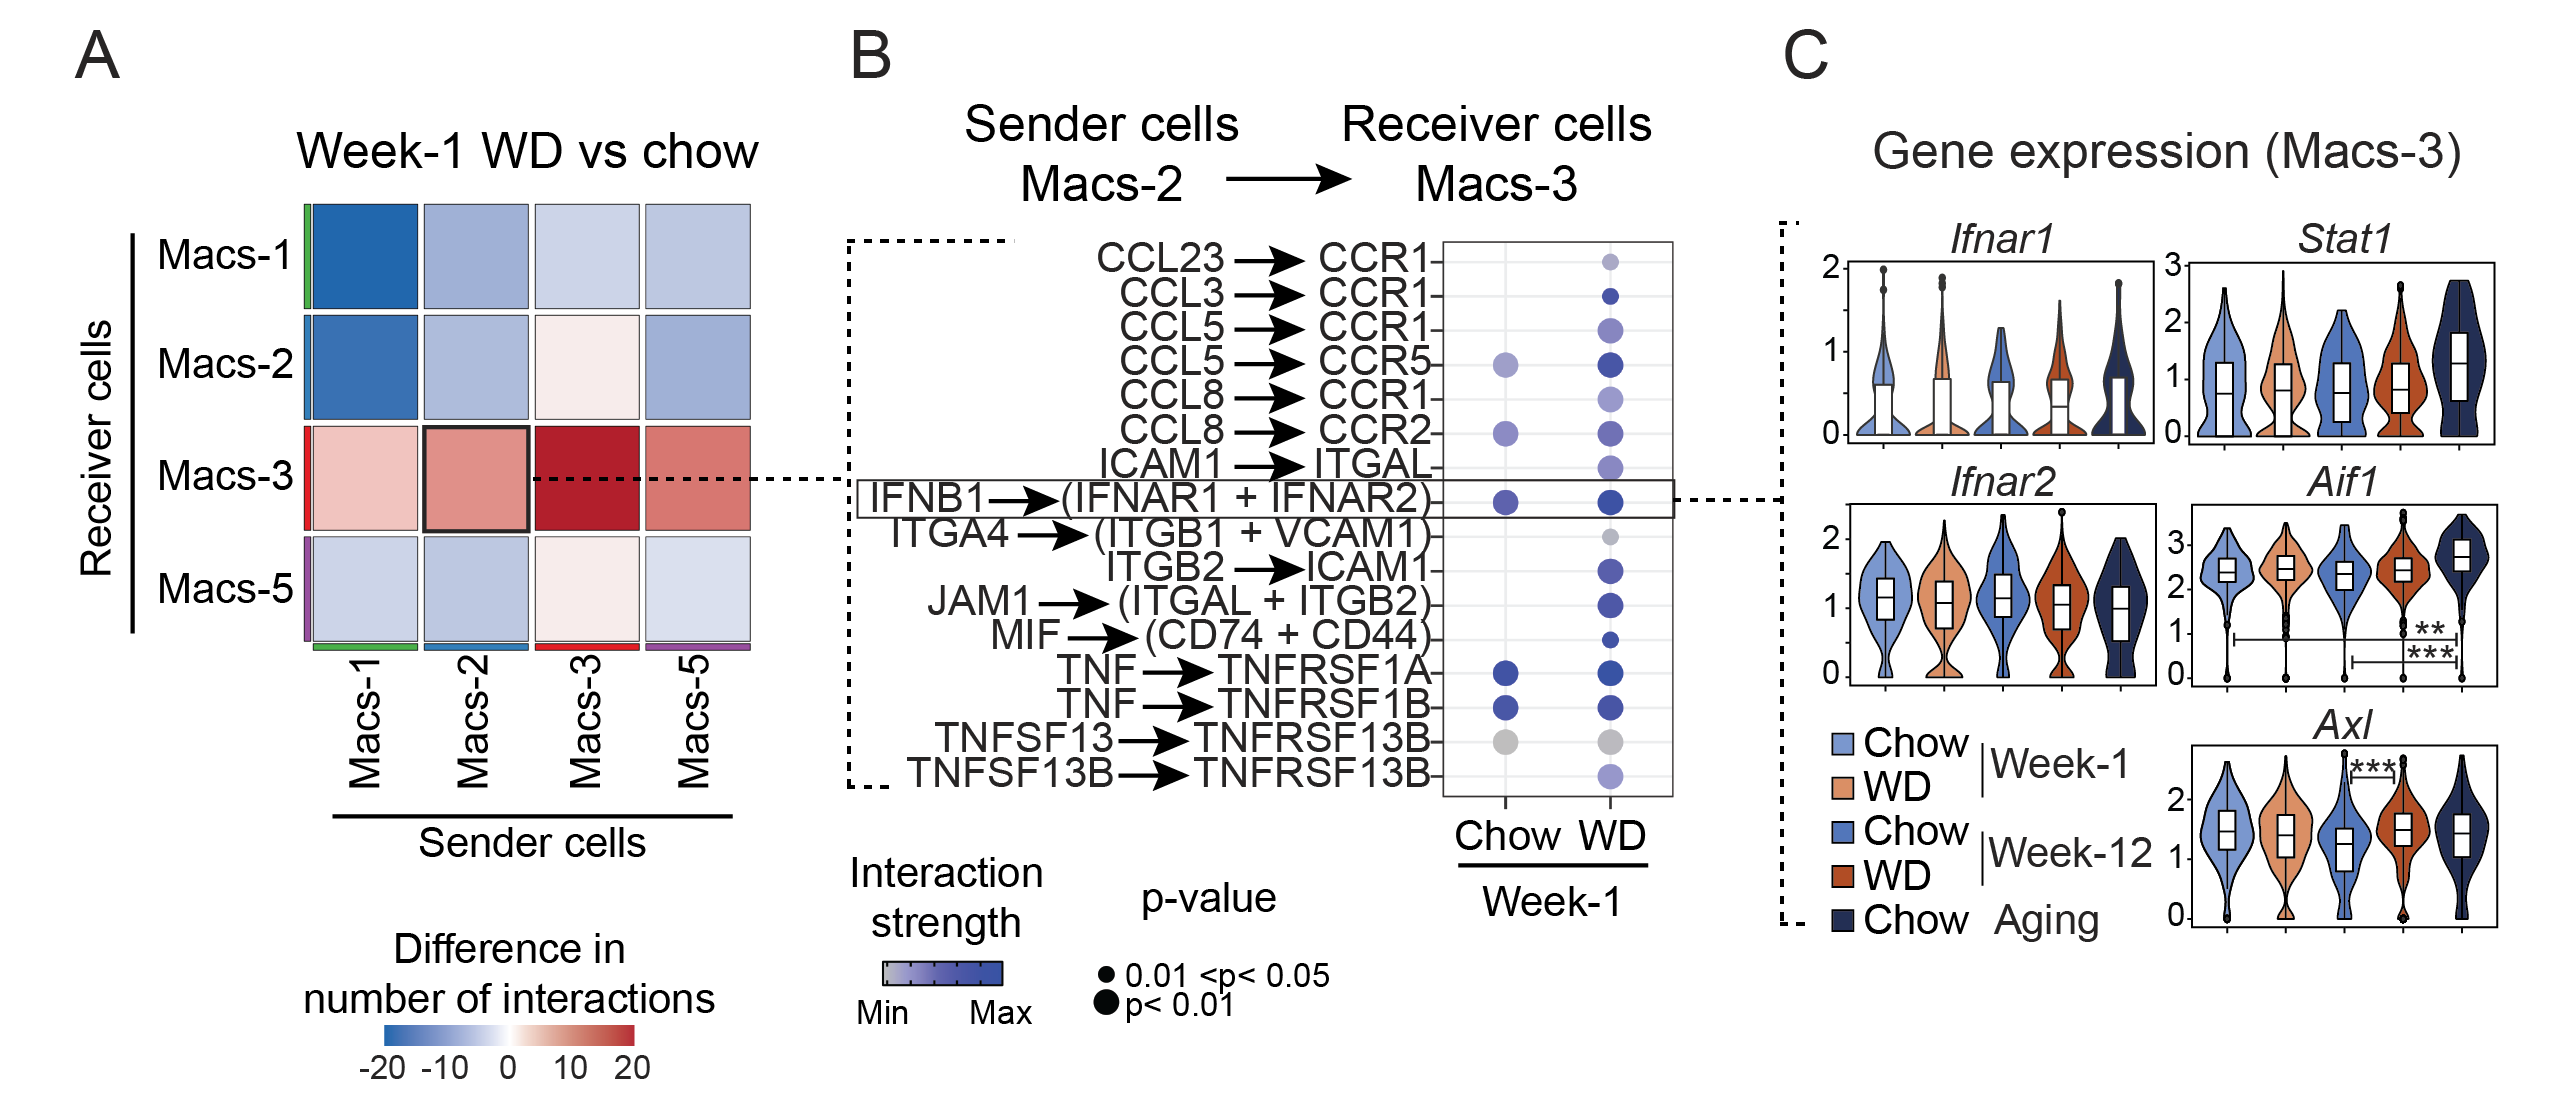
\includegraphics[width=\linewidth]{Chapter4/Fig/F2-6-01.png}
\caption[Intercellular interactions under acute overnutrition]{\textbf{Intercellular interactions under acute overnutrition.} \textbf{(A)} Heatmap depicting the difference in number of \gls{lr} interactions in the indicated macrophage sub-populations between the \gls{wd} cohorts compared to the chow diet cohorts after 1 week of feeding. In the color bar, the red (or blue) represents increased (or decreased) number of interactions in the \gls{wd} data compared to chow data. The cells from different biological replicate cohorts were pooled together for the analysis. \textbf{(B)}  Dot plot depicting the computed communication probability for the indicated \gls{lr} pairs which were enriched in the Week-1 \gls{wd} feeding cohorts, with signals from Macs-2 to Macs-3. The dot color and size represent the calculated communication probability and significance, respectively. p-values are computed from one-sided permutation test directly within CellChat. \textbf{(C)} Violin plots depicting the normalized expression of the highlighted receptor and associated signaling pathway genes in Macs-3, across the different experimental conditions.}
\label{fig:chp2_scrna_cellchat1}
\end{figure}

To investigate the effects of an acute \gls{wd} feeding regimen on the intercellular interactions between the sub-populations from the islet-intrinsic macrophages in the single-cell data, we performed differential interaction analysis between \gls{wd} and normal chow diet feeding after one week (W1), using CellChat \textbf{\cite{jin_cellchat_2023}}. We excluded the proliferative Macs-4 from subsequent \gls{lri} analysis. We observed an increased number of incoming signals into the inflammatory Macs-3 \textbf{(\autoref{fig:chp2_scrna_cellchat1} A)} as well as an increase in the incoming interaction strength in response to \gls{wd} feeding \textbf{(\autoref{fig:app_scrna_cellchat1}} left\textbf{)}. Conversely, Macs-1 and the Macs-2 sub-populations had reduced number of incoming signals \textbf{(\autoref{fig:chp2_scrna_cellchat1} A)} as well as reduced incoming interaction strength during acute overnutrition \textbf{(\autoref{fig:app_scrna_cellchat1}} left\textbf{)}. We were particularly interested in the intercellular communications between the two inflammatory macrophage sub-populations under acute \gls{wd} feeding. Therefore, we examined the up- and down-regulated \gls{lr} signaling pairs from Macs-2 to Macs-3 in the \gls{wd} compared to normal chow diet. Several interaction pairs such as cytokine:cytokine-receptors, \gls{ifn}:\gls{ifn}-receptors and \gls{tnf}:\gls{tnf}-receptors were enriched in response to \gls{wd} feeding between Macs-2 and Macs-3 \textbf{(\autoref{fig:chp2_scrna_cellchat1} B)}. Among these, notably, there was a significant enhancement in the signaling from the \textit{Ifnb1} expressing Macs-2 to the type-1 \gls{ifn} responsive Macs-3 macrophage sub-population, one week following the initiation of a \gls{wd}. This communication is characterized by the action of \gls{ifn}-$\beta$1 on \gls{ifn}A receptors \textbf{(\autoref{fig:chp2_scrna_cellchat1} B)}, which could expain the heightened type-1 \gls{ifn} response observed in Macs-3 \textbf{(\autoref{fig:chp2_scrna_macrophages_macs3_dge} A)}. Moreover, an increase in the expression levels of type-1 \gls{ifn} receptors and their downstream target genes (\textit{Stat1}) was detected in Macs-3 during acute \gls{wd} feeding \textbf{(\autoref{fig:chp2_scrna_cellchat1} C)}.\\

\par In summary, the interplay between the two distinct inflammatory macrophage sub-populations within the islets might possibly contribute to the \gls{wd}-induced activation of the type-1 \gls{ifn} response in Macs-3. 

\subsubsection{\large Intercellular interactions under chronic overnutrition}

The prolonged exposure to \gls{wd} feeding necessitates an investigation into its chronic effects on intercellular interactions within the islet niche. The sustained overstimulation from a \gls{wd} is likely to modify the interaction landscape between islet macrophages and T-cells, possibly leading to a persistent inflammatory state. Indeed, local T-cells have been shown to play an important role in driving inflammatory processes and insulin resistance by inducing proinflammatory cytokines and chemokines in metabolically active organs, such as the adipose tissue, liver and muscle \textbf{\cite{mclaughlin_t-cell_2014,wu_skeletal_2017,park_role_2022}}. This promotes recruitment and phenotypic changes of macrophages. Whether such a cellular crosstalk between macrophages and T-cells occurs in the pancreas, irrespective of within or around the islets, is unclear.\\

\par We therefore investigated the chronic effects of \gls{wd} feeding on the intercellular communications within the islets by performing a differential \gls{lri} analysis between \gls{wd}


\begin{figure}[t]
\centering
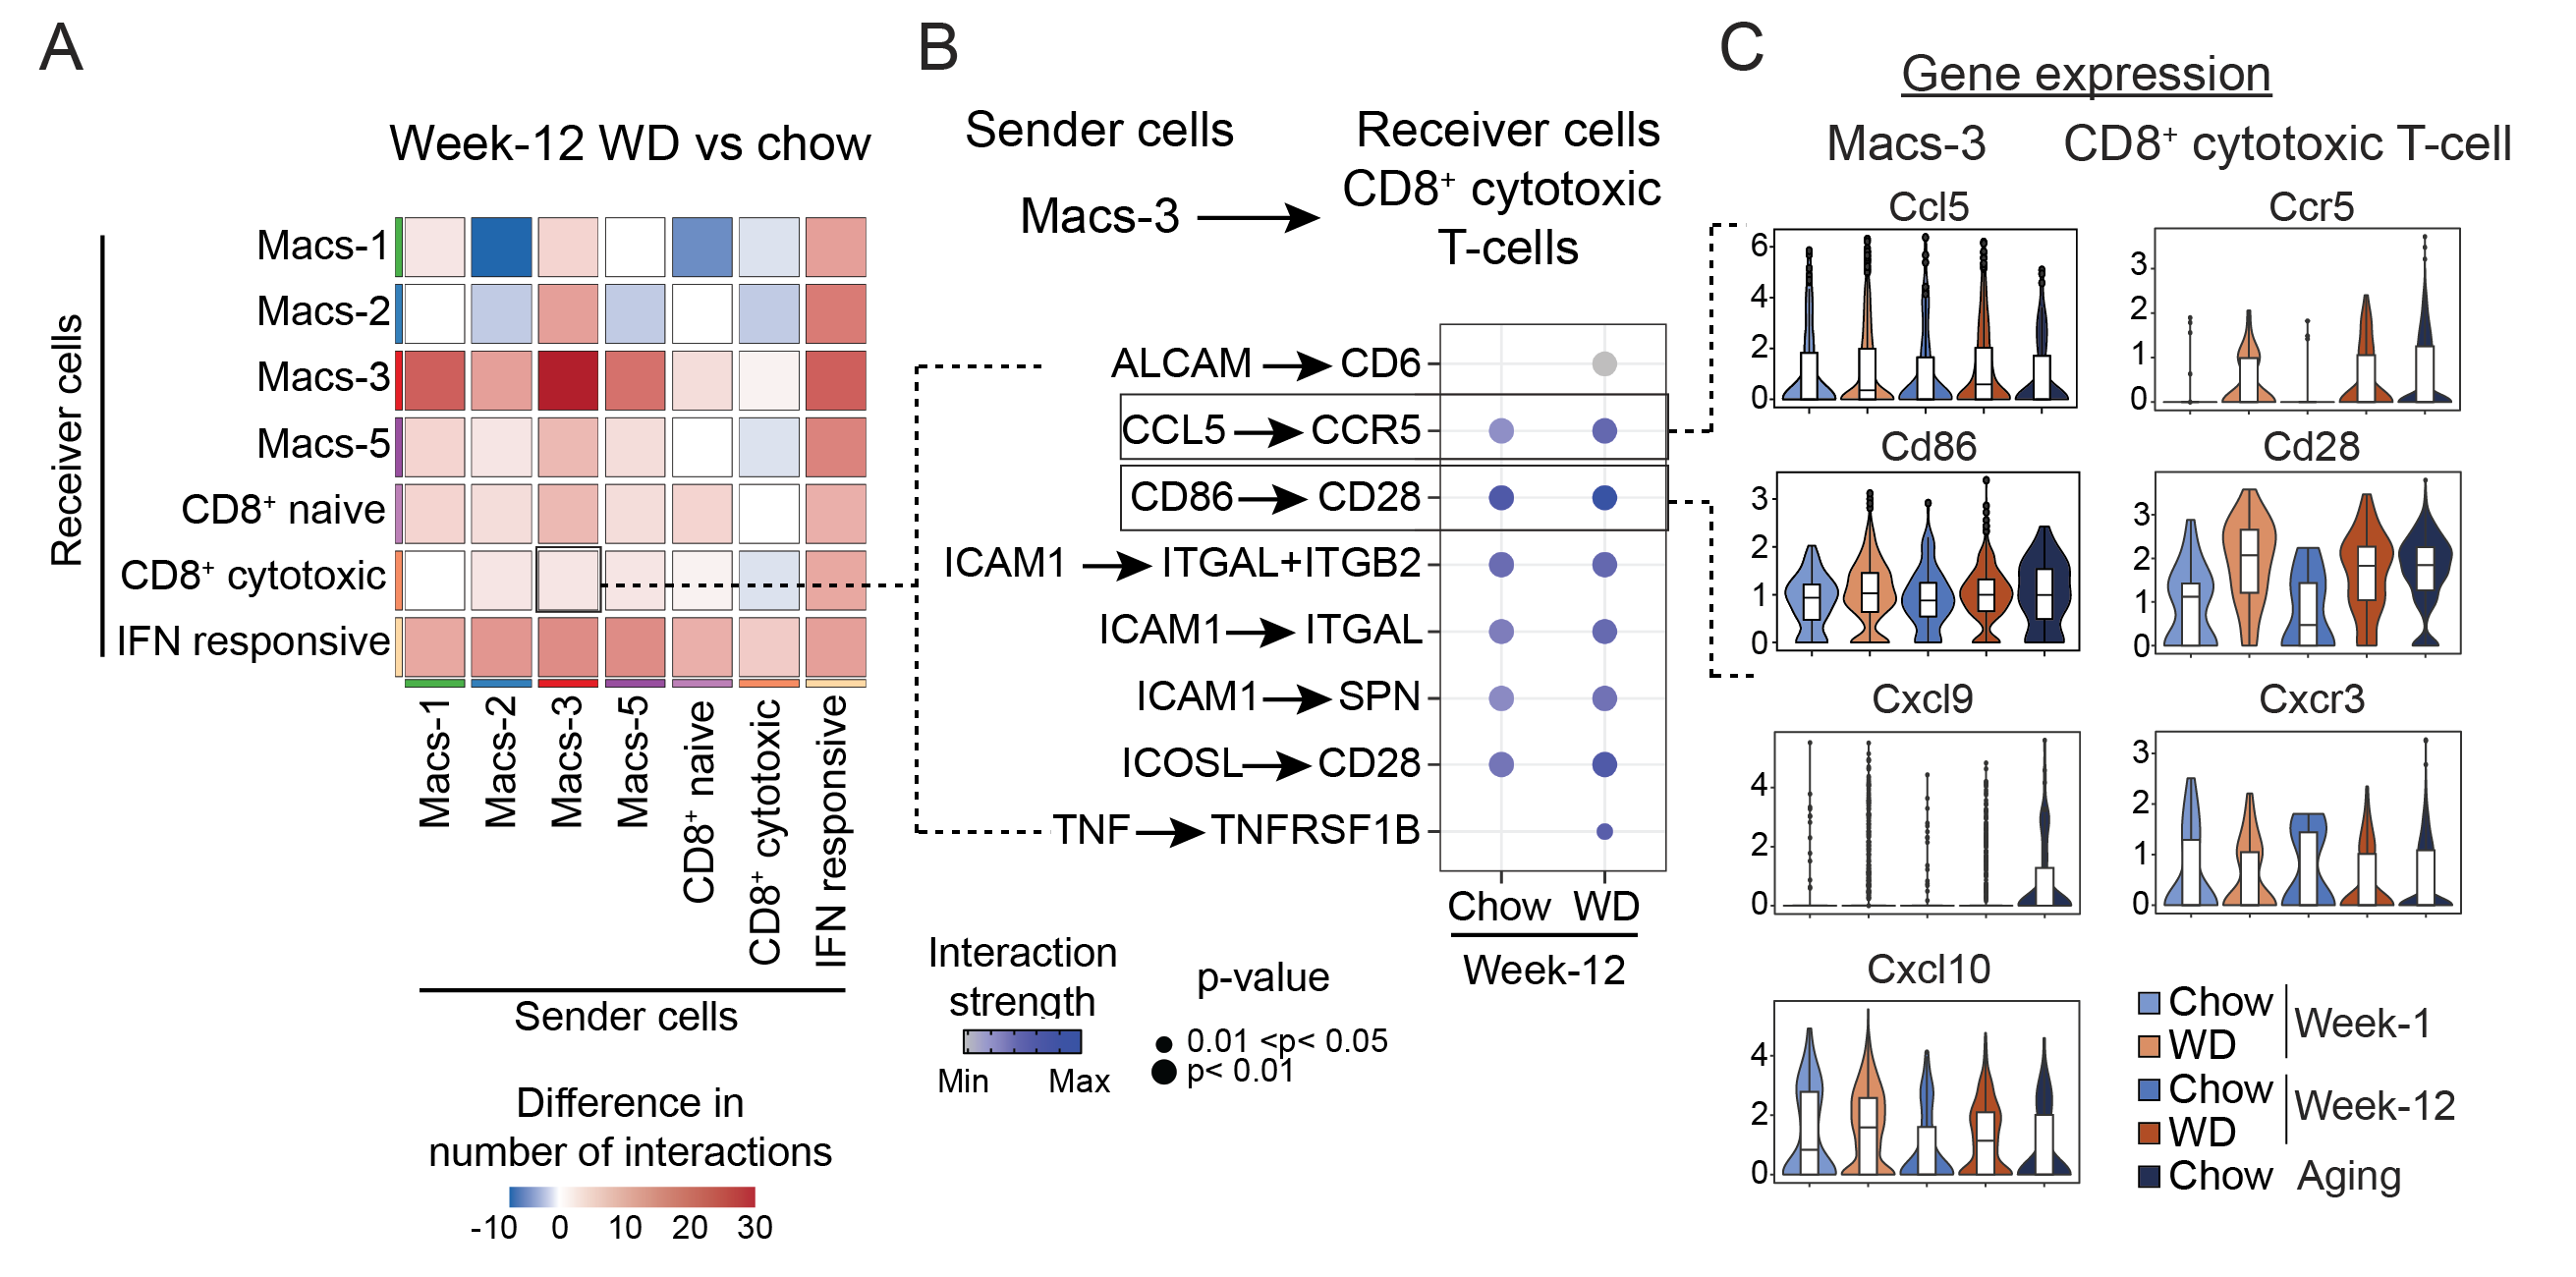
\includegraphics[width=\linewidth]{Chapter4/Fig/F2-7-01.png}
\caption[Intercellular interactions under chronic overnutrition]{\textbf{Intercellular interactions under chronic overnutrition.} \textbf{(A)} Heatmap depicting the difference in number of \gls{lr} interactions in the indicated macrophage and T-cell sub-populations between the \gls{wd} cohorts compared to the chow diet cohorts after 12 weeks of feeding. In the color bar, the red (or blue) represents increased (or decreased) number of interactions in the \gls{wd} data compared to chow data. The cells from different biological replicate cohorts were pooled together for the analysis. \textbf{(B)} Dot plot depicting the computed communication probability for the indicated \gls{lr} pairs which were enriched in the Week-12 \gls{wd} feeding cohorts, with signals from Macs-3 to CD8\textsuperscript{+} cytotoxic T-cells. The dot color and size represent the calculated communication probability and significance, respectively. p-values are computed from one-sided permutation test directly within CellChat. \textbf{(C)} Violin plots depicting the normalized expression of the highlighted ligands in Macs-3 and receptors in CD8\textsuperscript{+} cytotoxic T-cells in \textbf{(B)} across the different experimental conditions.}
\label{fig:chp2_scrna_cellchat2}
\end{figure}

and normal chow diet feeding after twelve weeks (W12), using CellChat \textbf{\cite{jin_cellchat_2023}}. Similar to the W1 analysis, we included all non-proliferating macrophage sub-populations and T-cells from the single-cell data. Compared to W1 feeding, the type-1 \gls{ifn}-responsive Macs-3 depicted an overall increase in numbers of outgoing and incoming interaction signals \textbf{(\autoref{fig:chp2_scrna_cellchat2} A)} as well an increase in their corresponding interaction strengths \textbf{(\autoref{fig:app_scrna_cellchat1}} middle\textbf{)}. To further explore the crosstalk between macrophages and T-cells, we focused on the intercellular interactions between Macs-3 and CD8\textsuperscript{+} cytotoxic T-cells. With the progression of overnutrition, the activated Macs-3 sub-population increased its communication with CD8\textsuperscript{+} cytotoxic T-cells, as evidenced by increased number of interactions \textbf{(\autoref{fig:chp2_scrna_cellchat2} A)}. Notable interactions between these two sub-populations comprise the action of C-C motif chemokine ligand 5 (CCL5) secreted by Macs-3 on the C-C chemokine receptor type 5 (CCR5) receptor present on CD8\textsuperscript{+} cytotoxic T-cells, as well as the engagement of the co-stimulatory signaling molecules CD86 on Macs-3 with CD28 on CD8\textsuperscript{+} cytotoxic T-cells, which are required for T-cell activation and survival \textbf{(\autoref{fig:chp2_scrna_cellchat2} B)} \textbf{\cite{sansom_cd28_2000}}. Within the Macs-3 sub-population, the expression of \textit{Ccl5} was exclusively triggered by \gls{wd} feeding, while \textit{Cd86} expression was common to both overnutrition and aging \textbf{(\autoref{fig:chp2_scrna_cellchat2} C)}. Additionally, the communication between Macs-3 and CD8\textsuperscript{+} cytotoxic T-cells featured a \gls{wd}-specific involvement of \textit{Cxcl10}, which acts through the \textit{Cxcr3} receptor on the CD8\textsuperscript{+} cytotoxic T-cells. Conversely, under aging conditions, \textit{Cxcl9} is the preferentially expressed ligand for \textit{Cxcr3} \textbf{(\autoref{fig:chp2_scrna_cellchat2} C)}.\\

\par It is well-established that \textit{Cxcl9} expression is triggered by the canonical type-1 \gls{ifn} pathway, whereas \textit{Ccl5} and \textit{Cxcl10} transcription is induced by the non-canonical type-1 \gls{ifn} signaling pathway \textbf{\cite{mazewski_type_2020}}, reflecting the distinct activation states of Macs-3 under the two different stress conditions \textbf{(\autoref{fig:chp2_scrna_macrophages_macs3_dge})}. Furthermore, the Macs-2 sub-population, which also exhibited non-canonical type-1 \gls{ifn} responses during overnutrition, up-regulated the transcription of \textit{Ccl5} and \textit{Cxcl10} in response to \gls{wd} compared to chow diet feeding and aging \textbf{(\autoref{fig:app_scrna_macrophages_macs2_dge})}. This suggests that Macs-2 cells may also contribute to the overnutrition- and aging- specific communication between macrophages and T-cells. Importantly, our \gls{imc} analysis revealed that F4/80\textsuperscript{-} and F4/80\textsuperscript{\textit{low}} macrophages, corresponding to the Macs-2 and Macs-3 sub-populations in the \gls{scr} data, respectively, show a positive correlation with CD8\textsuperscript{+} activated effector-like T-cells in the pancreatic tissue therefore indicating a mutual dependency between these sub-populations \textbf{(\autoref{fig:chp2_imc_correlation} A)}. Additionally, CD8\textsuperscript{+} and CD11c\textsuperscript{+} cells were frequently observed, both in the exocrine pancreas and within pancreatic islets and in close proximity to each other \textbf{(\autoref{fig:chp2_imc_correlation} B)}.\\% This further suggests the possibility of intercellular \gls{lri}s thereby perpetuating local islet inflammation in overnutrition.\\

% This suggests that the cytokine / chemokine-mediated communication between Macs-2 / Macs-3 sub-populations and the T-cells significantly differs between overnutrition and aging conditions, even though CD86 and CD28 mediated interactions remain consistent across these scenarios (\textbf{Fig.\ref{suppl_fig:cell_cell2}}).


\begin{figure}[t!]
\centering
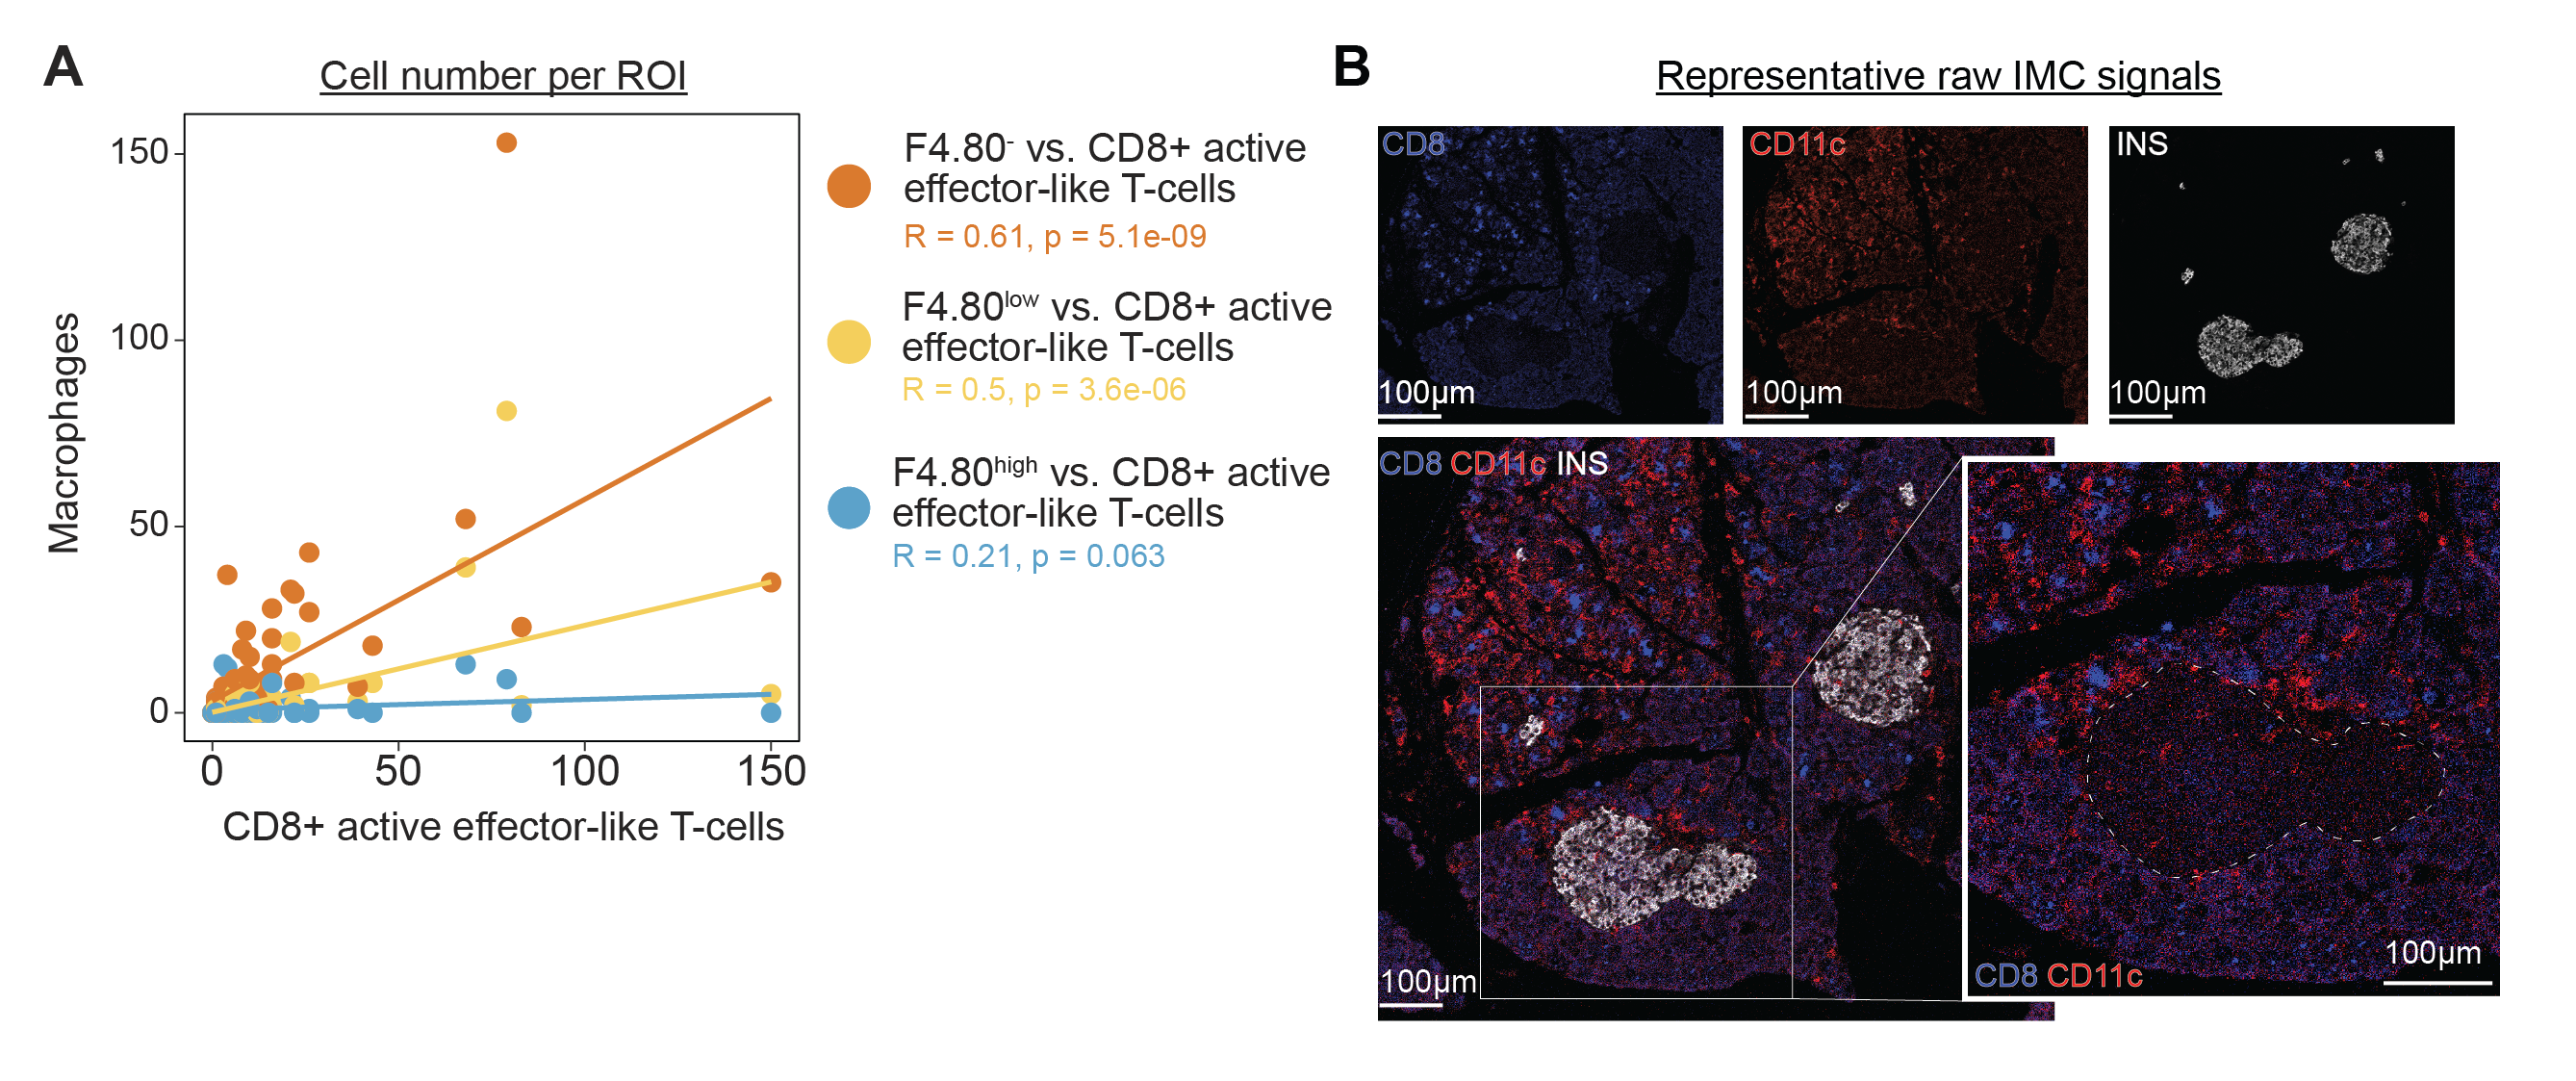
\includegraphics[width=\linewidth]{Chapter4/Fig/F2-8-01.png}
\caption[Co-localization of macrophages and T-cells within pancreas]{\textbf{Co-localization of macrophages and T-cells within pancreas and pancreatic islets.} \textbf{(A)} Scatter plot depicting the correlation between the counts of CD8\textsuperscript{+} activated effector-like T-cells and three macrophage sub-populations from the \gls{imc} analysis, within the same \glspl{roi}. Solid lines represent best fit in each correlation analysis. Pearson correlation coefficients and p-values for the corresponding macrophage sub-populations are included. \textbf{(B)} Representative \gls{roi} showing raw signals from the CD8 (blue), CD11c (red), and INS (white) channels. Scale bar, 100 \textmu m. \textit{This data and figure were originally generated by Dr. Matthias Barone and reused here with permission.}}
\label{fig:chp2_imc_correlation}

\end{figure}


\subsubsection{\large Intercellular interactions during aging}

%Observations from our data and evidence from a previous study points to the accumulation of T-cells in non-diabetic islets during aging \textbf{\cite{denroche_t_2021}}. Furthermore, another study indicated that 

\par  We examined intercellular interactions during aging compared to chow diet-fed non-aging cohorts for the non-proliferating macrophage and CD8\textsuperscript{+} T-cell sub-populations. Similar to the observations of increased interaction strengths in response to \gls{wd}, aging also resulted in similar increases in strengths of the incoming and outgoing interactions for the four macrophage sub-populations as well as the CD8\textsuperscript{+} naive and cytotoxic T-cells \textbf{(\autoref{fig:app_scrna_cellchat1}} right\textbf{)}. We observed that the CD8\textsuperscript{+} memory T-cells depicted the strongest interactions as well as a higher number of outgoing and incoming interactions amongst all the other sub-populations during aging \textbf{(\autoref{fig:chp2_scrna_cellchat3} A; \autoref{fig:app_scrna_cellchat1}} right\textbf{)}. This could be attributed to the aging-specific abundance of the CD8\textsuperscript{+} memory T-cells \textbf{(\autoref{fig:chp2_scrna_tcells1} B; \autoref{tab:app_scrna_cellnumbers})}. Similarly, despite the increase in number of interactions involving the \gls{ifn}-responsive T-cells during both, chronic \gls{wd} feeding and aging, we could not infer any significant signaling interactions using CellChat, possibly due to the overall low number of \gls{ifn}-responsive T-cells in the adult cohorts \textbf{(\autoref{fig:chp2_scrna_tcells1} B; \autoref{tab:app_scrna_cellnumbers})}. Interestingly, we observed more interactions in the aging cohort compared to adult cohorts of 10-week-old and 21-week-old mice in all sub-populations \textbf{(\autoref{fig:chp2_scrna_cellchat3} A)} indicating an altered landscape of immune crosstalk during aging.\\

\begin{figure}[b!]
\centering
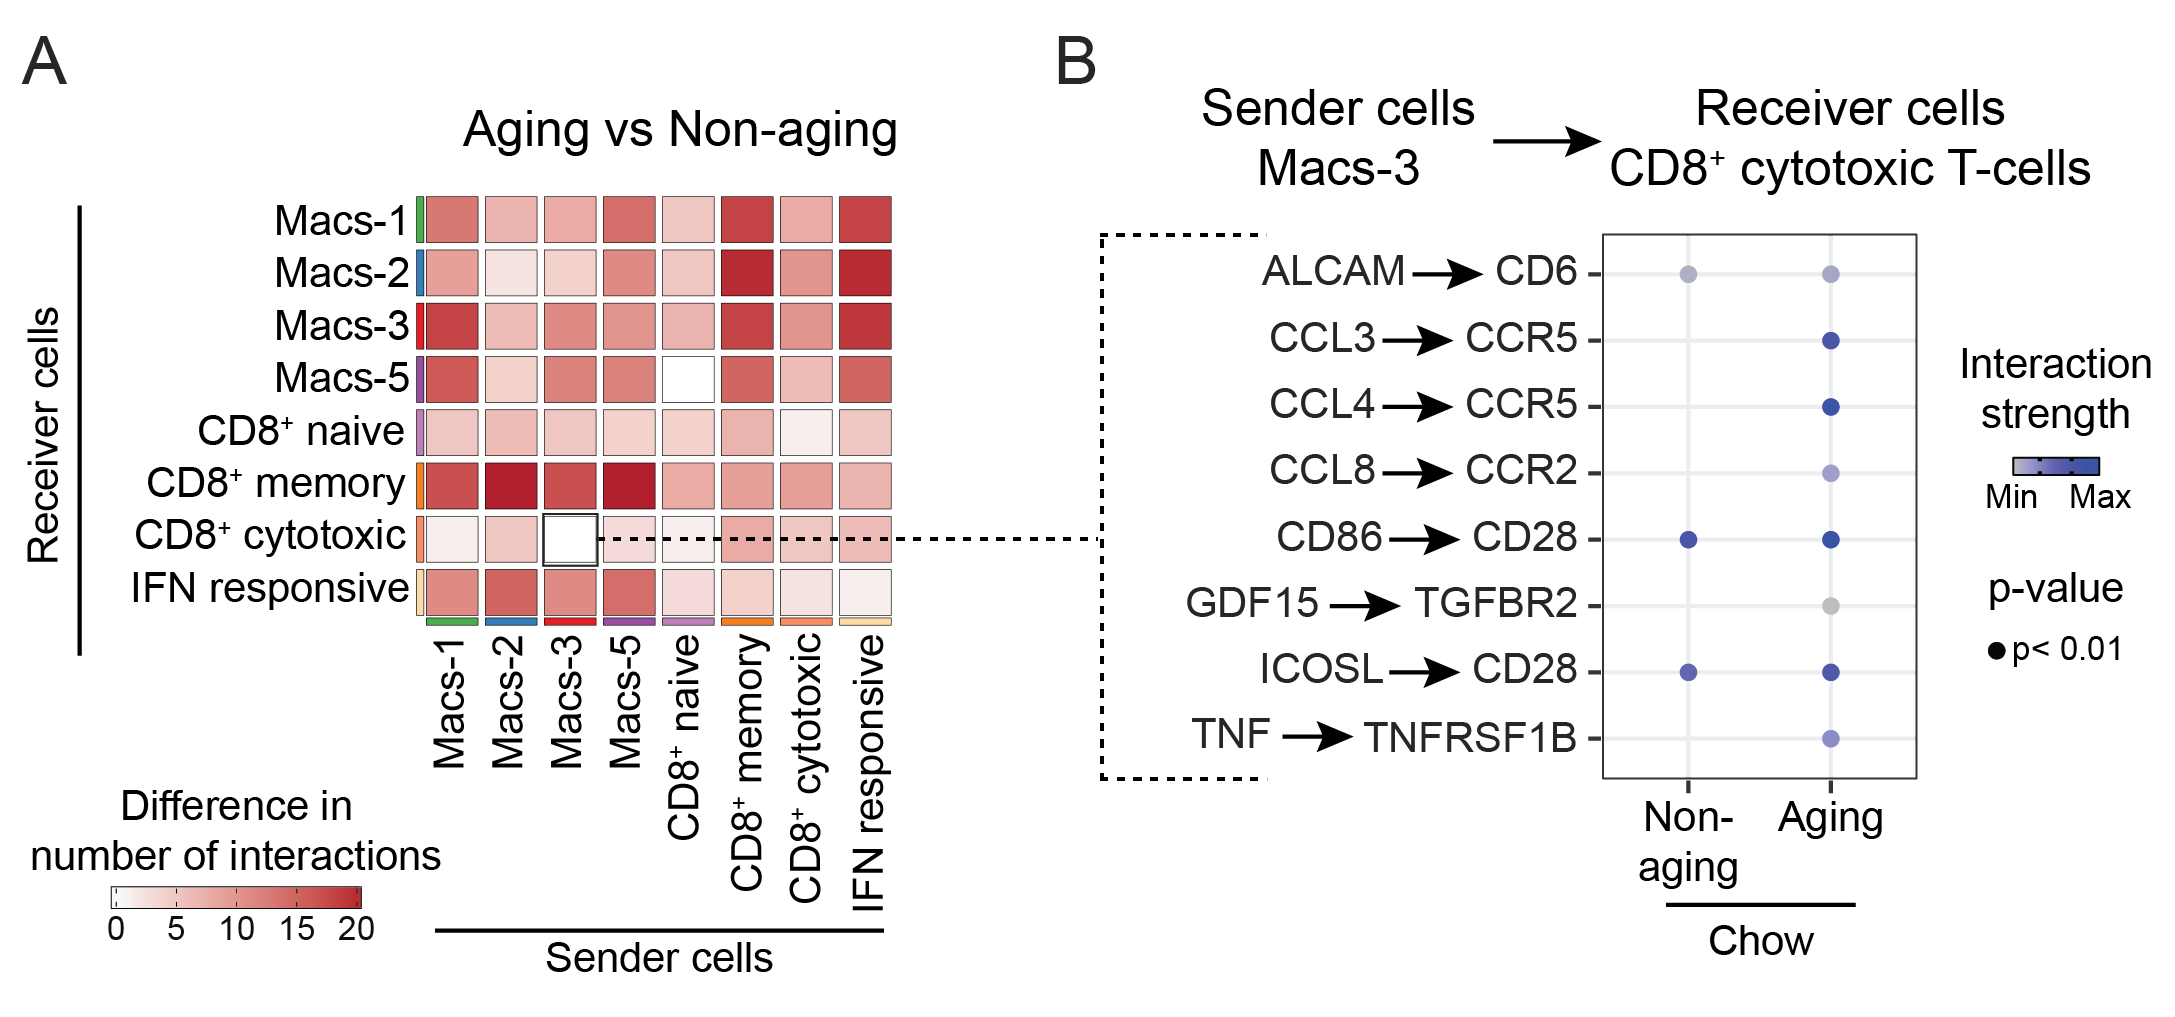
\includegraphics[width=\linewidth]{Chapter4/Fig/F2-A1-v3-02.png}
\caption[Intercellular interactions under aging]{\textbf{Intercellular interactions under aging.}
\textbf{(A)} Heatmap depicting the difference in number of \gls{lr} interactions in the indicated macrophage and T-cell sub-populations between the chow diet-fed aging cohorts compared to the chow diet-fed non-aging cohorts. In the color bar, the red represents the increased number of interactions in the aging data compared to non-aging data. The cells from different biological replicate cohorts were pooled together for the analysis. \textbf{(B)} Dot plot depicting the computed communication probability for the indicated \gls{lr} pairs which were enriched in aging, with signals from Macs-3 to CD8\textsuperscript{+}  cytotoxic T-cells. The dot color and size represent the calculated communication probability and significance, respectively. p-values are computed from one-sided permutation test directly within CellChat.}
\label{fig:chp2_scrna_cellchat3}
\end{figure}

\par To examine the overlap of intercellular interactions between macrophages and T-cells during overnutrition and aging, we focused on interactions between Macs-3 and CD8\textsuperscript{+} cytotoxic T-cells. In contrast to the observations of \gls{wd}-specific expression of \textit{Ccl5} \textbf{(\autoref{fig:chp2_scrna_cellchat2} C)}, interactions that were found to be enriched between Macs-3 and CD8\textsuperscript{+} cytotoxic T-cells during aging did not include CCL5. Instead, Macs-3 secreted other chemokines such as CCL3 and CCL4 which was predicted to interact with the CCR5 receptor, and CCL8 was predicted to interact with the CCR2 receptor on the cytotoxic T-cells \textbf{(\autoref{fig:chp2_scrna_cellchat3} B)}. Despite this contrast in interactions in response to \gls{wd} feeding and aging, the CD86-CD28 co-stimulatory interaction was shared between the two metabolic stresses \textbf{(\autoref{fig:chp2_scrna_cellchat3} B)}.\\

\par Collectively, our \gls{lri} analysis suggests that both of the inflammatory macrophage sub-populations in the pancreas and pancreatic islets actively communicate with cytotoxic T-cells. This communication relies on distinct chemokine / cytokine profiles under \gls{wd} and aging conditions, but utilizes the same co-stimulatory mechanisms. 

\clearpage

\section[Summary]{Summary}
\label{sec:chp2_summary}
\vspace{-5pt}
\par In this study, we employed \gls{imc} and \gls{scr} to profile immune cells within pancreatic tissue and pancreatic islets. Our goal was to integrate their phenotypic characteristics with spatial localization, providing a more comprehensive understanding of their roles under these conditions. Our multi-modal approach allowed us to characterize the heterogeneous landscape of immune cell types in the pancreatic tissue as well as within the islet niche. We identified several macrophage and T-cell sub-populations in both, \gls{imc} and \gls{scr} data, and linked them based on the expression of the several characteristic markers in the \gls{imc} panel as well as the corresponding genes in \gls{scr}.\\

\par More importantly, we discovered that:

\begin{enumerate}
    \item Obesity, induced by \gls{wd} feeding, significantly accelerated the age-dependent accumulation of a pro-inflammatory F4/80\textsuperscript{\textit{low}} Macs-3 macrophage sub-population and CD8\textsuperscript{+} cytotoxic T-cells. This likely suggests the stronger impact of diet on immune cell dynamics in the pancreatic tissue.
    \item The pro-inflammatory Macs-3 depicted distinct type-1 \gls{ifn} responses dependent on the stimulus: aging induced a canonical response with \textit{Stat1} activation, whereas overnutrition resulted in a non-canonical response marked by \textit{Stat3} activation and involved alternative pathways such as \gls{mtor} signaling. Our findings suggest that the type-1 \gls{ifn} response in islet-associated macrophages during metaflammation may be more strongly altered compared to the response in inflammaging.
    \item The numbers of F4/80\textsuperscript{\textit{low}} macrophages and the CD8\textsuperscript{+} activated-effector like T-cells exhibited positive correlation in the \gls{imc} data and intercellular interaction analyses between Macs-3 and CD8\textsuperscript{+} cytotoxic T-cells revealed a possible non-canonical type-1 \gls{ifn} signaling cascade during \gls{wd} feeding involving CCL5-CCR5 interaction along with the co-stimulatory mechanism of CD86-CD28.
\end{enumerate}

\par These findings are crucial for understanding the progression and development of \gls{t2d} and underscores the importance of considering both dietary and age-related factors in diabetes research and their roles in modulating inflammation that affects disease progression.\\


%Furthermore, our multi-modal approach also provided a detailed spatio-temporal characterization of other immune cells, islet endocrine cells as well as other relevant cell populations during overnutrition and aging

\newpage\null\thispagestyle{empty}


% By combining single cell expression profiling and common genetic variation of over one hundred individuals we can begin to assess the impact of genetic variability on expression in a continuous manner across early human development.
% We have imputed genotypes for all of our 125 samples \cite{kilpinen2017common}, so this study allows discovery of single cell eQTL along differentiation. 
% Using the developmental stages just described and methods similar to those described in the previous chapter, we mapped eQTL in each of the \gls{ipsc}, mesendo and defendo populations, yielding 1,833, 1,702 and 1,342 eGenes, respectively. 
% Briefly, we quantified each gene’s average expression level for each donor, experiment, and differentiation stage\footnote{This approach is the same as what is described in the first part of \textbf{Chapter \ref{chapter3}}, and similar to the `dr-mean' described in \textbf{section \ref{sec:best_practice}}, except that the aggregation is done at the experiment level rather than the sequencing run level.}, before using a linear mixed model to test for \textit{cis} eQTL, adapting approaches used for bulk RNA-seq profiles (+ and - 250 kb, MAF >5\% \cite{kilpinen2017common}).\\

% For comparison, we also performed eQTL mapping in cells collected on day1 and day3, i.e. the experimental time points commonly used to identify cells at mesendo and defendo stages \cite{hannan2013production}.
% Interestingly, this approach identified markedly fewer eGenes: 1,181 eGenes at day1, and 631 eGenes at day3.
% These results demonstrate the power of using the single-cell RNA-seq profiles to define relatively homogeneous differentiation stages in a data-driven manner (\textbf{Fig. \ref{fig:endodiff_stage_eqtl}}). 
% Notably, this observation was not merely a consequence of differences in the number of cells or donors considered in each cell population (\textbf{Fig. \ref{fig:endodiff_stage_eqtl}}). \\

% \begin{figure}[h]
% \centering
% \includegraphics[width=14cm]{Chapter4/Fig/endodiff_eqtl.png}
% \caption[eQTL maps of iPSC, mesendo, defendo]{\textbf{Mapping single cell eQTL at different developmental stages.}\\
% (a) Illustration of the single cell eQTL mapping strategy at various stages of differentiation.
% Shown is an example of a defendo-specific eQTL. 
% Box plots of gene expression stratified by the allelic state of
% rs9648854 at each stage, showing an association between rs9648854 and \textit{CNTNAP2} expression at the defendo stage, but not at earlier stages. 
% (b) Comparison of eQTL mapping using different strata of all cells.
% The use of pseudotime-based stages increases the number of detectable eQTL, compared to using the corresponding time point of collection.
% Bar plots represent number of eGenes (genes with at least one eQTL, at FDR < 10\%).
% (c) Similar to b, the number of donors for which gene expression data were assayed at day0, day1, and day3, compared to the number of donors in the pseudotime-inferred mesendo and defendo stages.
% (d) As for (c), with the number of cells.
% \url{https://github.com/ebiwd/EBI-Icon-fonts} by EBI Web Development is licensed under CC BY 4.0. }
% \label{fig:endodiff_stage_eqtl}
% \end{figure}

% Profiling multiple stages of endoderm differentiation allowed us to assess at which stage along this process individual eQTL can be detected as well as the level of sharing of genetic signal across time. 
% We observed substantial regulatory and transcriptional remodelling upon endoderm differentiation of iPSCs, with over 30\% of eQTL being specific to a single stage.
% To define pairwise replication (and conversely specificity) between two sets of test results we considered nominal significance (p value < 0.05) and consistent direction of the effect size.
% Importantly, we observed that stage-specificity of eQTL was not significantly explained by stage-specific gene expression (\textbf{Fig. \ref{fig:endodiff_stage_specific_eqtl}}).
% Our differentiation time course covers developmental stages that have never before been accessible to genetic analyses of molecular traits and thus this study provides the first eQTL maps at mesendoderm and definitive endoderm.
% We next explored whether any of the eQTL identified in these two studies were novel, and found that 349 of them have not been reported in either a recent iPSC eQTL study based on bulk RNA-seq \cite{mirauta2018population}, or in a compendium of eQTL identified from 49 tissues as part of the GTEx project \cite{gtex2017genetic}.
% An eQTL was defined as novel when it was not reported as lead variant (FDR < 10\%) in any of the tissues considered nor was it in \gls{ld} (see \textbf{section \ref{sec:gwas}}) with any reported lead variant, \gls{ld} assessed using $r^2<0.2$.\\

% Finally, we investigated the presence of lead switching events.
% These correspond to two distinct genetic variants that are identified as lead eQTL for the same gene at different stages of differentiation (at LD: $r^2<0.2$),
% We found lead switching events for 155 eGenes (an example in iPSC and defendo is illustrated in \textbf{Fig. \ref{fig:endodiff_stage_specific_eqtl}}). 
% To explore the potential regulatory role of these variants, we investigated whether the corresponding genetic loci also featured changes in histone modifications during differentiation. 
% To do so, we used ChIP-Sequencing to profile five histone modifications that are associated with promoter and enhancer usage (H3K27ac, H3K4me1, H3K4me3, H3K27me3, and H3K36me3) in human embryonic stem cells (hESCs) that were differentiated towards endoderm (using the same protocol employed above) and measured at equivalent time points (i.e. day0, day1, day2, day3, see \textbf{section \ref{sec:endodiff_chipseq}} for detailed experimental methods). 
% Interestingly, we observed corresponding changes in the epigenetic landscape for 20 of the lead switching events (i.e. stage-specific lead variants overlapped with stage-specific changes in histone modification status), suggesting a direct mechanism (\textbf{Fig. \ref{fig:endodiff_stage_specific_eqtl}}).

% \begin{figure}[htbp]
% \centering
% \includegraphics[width=12cm]{Chapter4/Fig/endodiff_stage_specific.png}
% \caption[Stage-specific eQTL]{\textbf{Stage-specific eQTL.}\\
% (a) Proportion of eQTL that are specific to a single stage, shared across two
% stages, or observed across all stages (sharing defined as a lead eQTL variant at one stage with nominal p value < 0.05 and consistent direction
% at another stage).
% (b) Proportion of stage-specific eGenes (genes with a stage-specific eQTL) that are expressed only at a single stage, expressed at two stages, or expressed at all stages. 
% Expressed is defined as normalised log2(CPM+1) > 2. 
% CPM: counts per million.
% (c) A lead switching event consistent with epigenetic remodelling. 
% The overlap of H3K4me1 with the eQTL SNPs across differentiation time points is shown by the coloured bars.}
% \label{fig:endodiff_stage_specific_eqtl}
% \end{figure}
% The availability of large numbers of cells per donor across a continuous differentiation trajectory from pluripotent stage to definitive endoderm enabled the analysis of dynamic changes of eQTL strength at fine-grained resolution. 
% To formally test for eQTL effects that change dynamically across differentiation (dynamic eQTL), we tested for associations between pseudotime (both linear and quadratic) and the genetic effect size using allele-specific expression (ASE) and a linear model (see \textbf{Box \ref{box:ase}}):

% \begin{equation}\label{eq:endodiff_ase_pseudotime}
%     \mathrm{ASE} = \alpha_1 \mathrm{pseudotime} + \alpha_2 \mathrm{pseudotime}^2 + \boldsymbol{\psi},
% \end{equation}

% where the genetic effect is defined based on \gls{ase} at the level of single cells, i.e. quantified as fractional read counts overlapping each allele for a given gene-SNP pair (see details in \textbf{Box \ref{box:ase}}).
% We assessed significance using a likelihood ratio test with two degrees of freedoom (i.e. $H_0: \alpha_1 = \alpha_2 = 0$). 
% For this analysis, we focused on the joint set of 4,422 eQTL lead variants (4,470 SNP-gene pairs) discovered at the iPSC, mesendo, and defendo stages and explored how they were modulated by developmental time (using our inferred pseudotime).
% In this way, we uncovered a total of 899 time dynamic eQTL at FDR < 10\%, including a substantial fraction of eQTL that were not identified as stage-specific by the discrete approach previously used (\textbf{page \pageref{fig:endodiff_stage_specific_eqtl}}).
% This analysis is somewhat complementary to the eQTL map perfomed on discrete differentiation stages (\textbf{Fig. \ref{fig:endodiff_stage_eqtl}}), which identified substantial stage-specific effects (\textbf{Fig. \ref{fig:endodiff_stage_specific_eqtl}}).
% Namely, we observe that in general stage-specific effects are weaker and unique to certain cell types.
% In contrast, the dynamic eQTL identified are detected to a certain extent across all cell types, but the strength of the effect is modulated by differentiation time. \\

% One obvious explanation for these subtle dynamic changes could be that they are simply reflecting changes in overall expression. 
% To visualise this, we used a sliding-window approach. 
% Because we need a rather large amount of cells to reliably estimate expression abundance for each individual, we slide a window containing 25\% of the cells along pseudotime by a step of 2.5\% cells.
% In each window, we considered average expression quantifications and estimate genetic effects using eQTL mapping, essentially performing the same analysis we performed in developmental stages in \textbf{section \ref{sec:endodiff_eqtl}}, now in each window.
% In parallel, we reassessed each eQTL in each window taking advantage of the full length transcript sequencing to measure \gls{ase}.
% Here, in each window, we quantified the deviation from 0.5 of the expression of the minor allele at the eQTL (ratio of reads phased to eQTL variants, \textbf{Fig. \ref{fig:endodiff_sliding_window}}). 
% Notably, ASE can be quantified in each cell and is independent of expression level, thus mitigating technical correlations between differentiation stage and genetic effect estimates (\textbf{Box \ref{box:ase}}). 

%****** Box on ASE to quantify genetic effects ******

% \newpage

% \begin{Comment}
% \hspace{-2.5mm}\textbf{Box\ref{box:ase}: Quantifying genetic effects using ASE}\label{box:ase}\\
% \small
% When full-transcript (phased) data is available, \gls{ase} can be used to quantify the genetic effect of a variant on expression as a single ratio, by quantifying the relative expression of one allele over the other.
% For a given eQTL - and the corresponding eQTL variant and eGene -  we i) select individuals that are heterozygous at the eQTL SNP of interest, ii) consider all exonic heterozygous variants on the corresponding eGene, iii) map reads to these SNPs, iv) aggregate all reads coming from the same chromosome and v) compute the ratio. 
% Conventionally, we look at ratios < 0.5 i.e. in the numerator goes the allele with fewer reads mapped to it:

% \vspace{5mm}

% \includegraphics[width=15cm]{Chapter4/Fig/ASE.png}

% If one of these alleles is more responsive to a particular environmental factor (e.g. because of preferential transcription factor binding), then \gls{ase} is expected to vary consistently with that factor. 
% This observation has previously been used to identify GxE interactions in gene expression across individuals \cite{knowles2017allele}. 
% Critically, these \gls{ase} tests are internally matched, because potentially confounding batch effects and technical variation should affect both alleles in each cell similarly.
% Additionally, this test increases power by reducing the number of parameters to estimate, i.e. instead of the standard test for interactions:  

% \begin{equation*}
%     \mathrm{expression} = \sum_{k=1}^{K} \mathbf{e}_k\alpha_k + \mathbf{g}\beta +
%     \sum_{k=1}^{K} \mathbf{g} \odot \mathbf{e}_k\gamma_k + \boldsymbol{\psi},
% \end{equation*}

% where for each of K environments $\mathbf{e}_k$ two terms must be added (to account for E and GxE), resulting in (2*K + 2) parameters needing to be estimated (including one effect size $\beta$ and the variance explained by the noise term $\sigma_n^2$, from $\boldsymbol{\psi} \sim \mathcal{N}(\mathbf{0}, \sigma_n^2\mathbf{I_n})$), we can run:

% \begin{equation*}
%     \mathrm{ASE} = \sum_{k=1}^{K} \mathbf{e}_k\alpha_k + \boldsymbol{\psi}, 
% \end{equation*}
% where we can test directly the effect of the K environments on ASE and therefore only K+1 parameters need estimation (the K $\alpha_k$'s and $\sigma_n^2$).

% \end{Comment}

% \begin{figure}[h]
% \centering
% \includegraphics[width=15.5cm]{Chapter4/Fig/endodiff_running_average.png}
% \caption[Schematic of the sliding window approach]{\textbf{Schematic of the sliding window approach.}\\
% Cells are binned based on pseudotime ordering, to (a) quantify average expression, (b) perform eQTL mapping, and (c) quantify average ASE.
% Each bin includes 25\% of cells, binned at incremental steps of 2.5\%.}
% \label{fig:endodiff_sliding_window}
% \end{figure}

% Both methods result in a measure of genetic effect dynamics, i.e. changing strength of genetic effects along differentiation. 
% Reassuringly, the two approaches were highly consistent across pseudotime (\textbf{Fig. \ref{fig:endodiff_dynamic_eqtl}}).
% To explore this hypothesis, we clustered the top dynamic eQTL (FDR <1\%) jointly based on both the relative gene expression dynamics (global expression changes along pseudotime, quantified in sliding windows as above), and on the genetic effect dynamics (using ASE). 
% This identified four basic dynamic patterns (\textbf{Fig. \ref{fig:endodiff_dynamic_eqtl}}): decreasing early (cluster A), decreasing late (cluster B), transiently increasing (cluster C), and increasing (cluster D). 
% \begin{figure}[htbp]
% \centering
% \includegraphics[width=15.5cm]{Chapter4/Fig/endodiff_pseudo_heatmap.png}
% \caption[Dynamic eQTL]{\textbf{Dynamic eQTL.}\\
% Clustered heatmap of global expression levels, eQTL effect sizes, and ASE across pseudotime for the top 311 genes with the strongest dynamic eQTL effects (FDR < 1\%; out of 785 at FDR < 10\%). 
% For each gene, the dynamic profiles of gene expression and ASE were jointly grouped using clustering analysis, with 4 clusters. 
% The membership of a genes's expression and ASE dynamics to one of these clusters is shown by colours in the right-hand panel. 
% All values in the heatmaps are z-scores, normalised by gene (row). 
% In particular, for ASE, average ASE values are plotted such that red indicates highest deviation from 0.5.
% The diagram in the top right summarises the four identified cluster dynamics, displaying the average dynamic profile of each cluster, computed as the average across z-score normalised gene expression/ASE profiles. 
% Selected examples of the dynamics of allele expression for different cluster-combinations are shown in the bottom right panel.
% Shaded regions indicate standard error (+/- 1 SEM).
% This figure is based on one by Daniel Seaton.}
% \label{fig:endodiff_dynamic_eqtl}
% \end{figure}
% As expected, stage-specific eQTL were grouped together in particular clusters (e.g. defendo specific eQTL in cluster D, \textbf{Fig. \ref{fig:endodiff_dynamic_eqtl_enrichment}}). 
% Notably, the dynamic profiles of gene expression and those of eQTL effects tended to be distinct, demonstrating that expression level is not the primary mechanism controlling variation in genetic effects. 
% In particular, genetic effects were not most pronounced when gene expression was high (\textbf{Fig. \ref{fig:endodiff_dynamic_eqtl}}).
% Distinct combinations of expression and eQTL dynamics result in different patterns of allelic expression over time. 
% This is illustrated by the mesendoderm-specific eQTL for \textit{VAT1L}. 
% Overall expression of \textit{VAT1L} decreases during differentiation, but expression of the alternative allele is repressed more quickly than that of the reference allele (\textbf{Fig. \ref{fig:endodiff_dynamic_eqtl}}). 
% This illustrates how \textit{cis} regulatory sequence variation can modulates the timing of expression changes in response to differentiation, similar to observations previously made in \textit{C. elegans} using recombinant inbred lines \cite{francesconi2014effects}. 
% In other cases, the genetic effect coincides with high or low expression, for example in the cases of \textit{THUMPD1} and \textit{PHC2} (\textbf{Fig. \ref{fig:endodiff_dynamic_eqtl}}). 
% These examples illustrate how common genetic variation is closely linked to the dynamics of gene regulation. 
% % \\

% We next asked whether dynamic eQTL were located in specific regulatory regions. 
% To do this, we evaluated the overlap of our identified dynamic eQTL with epigenetic marks defined using the hESC differentiation time series\footnote{using bulk, at equivalent time points along endoderm differentiation, see \textbf{section \ref{sec:endodiff_chipseq}} for methods.} (\textbf{Fig. \ref{fig:endodiff_dynamic_eqtl_enrichment}}). 
% This revealed an enrichment of dynamic eQTL in enhancer (i.e. H3K27ac and H3K4me1), and promoter (H3K4me3) marks as compared to non-dynamic eQTL (i.e. eQTL we identified which did not display dynamic changes along pseudotime, \textbf{Fig. \ref{fig:endodiff_dynamic_eqtl_enrichment}}), consistent with these SNPs being located in active regulatory elements.

% \vspace{2mm}

% \begin{figure}[htbp]
% \centering
% \includegraphics[width=15cm]{Chapter4/Fig/endodiff_dynamic_enrich.png}
% \caption[Characterisation of dynamic eQTL]{\textbf{Characterisation of dynamic eQTL.}\\
% (a) Summary of the identified cluster dynamics\footnotemark and assignment of stage-specific eQTLs to dynamic eQTL clusters. 
% The numbers of each of the 3 classes of stage-specific eQTL (i.e. iPSC-, mesendo- , and defendo-specific eQTLs) that are assigned to each of the 4 dynamic eQTL clusters.
% (b) Number of genes categorised by the combination of expression and ASE cluster from (a). 
% Average dynamics of expression clusters (rows) and ASE clusters (columns) are shown.
% (c) Overlap of dynamic eQTL variants from a with histone marks.
% The odds ratio compared to the background of all other eQTL variants is shown (*p value < 0.01; **p value < $1x10^{-4}$; Fisher’s exact test).}
% \label{fig:endodiff_dynamic_eqtl_enrichment}
% \end{figure}

% \footnotetext{displaying the average dynamic profile of each cluster, computed as the average values across z-score normalised gene expression/ASE profiles.}
% Cells, that make up the tissues, communicate through signaling molecules like ligands and receptors \textbf{\cite{armingol_deciphering_2021,armingol_diversification_2024}}, allowing cells to maintain homeostasis, respond to internal and external perturbations, and enabling proper tissue function. These cell-cell interactions (CCIs) culminate in altered gene expression \textbf{\cite{armingol_deciphering_2021,armingol_diversification_2024}}, and therefore it is crucial to understand how cells interact and communicate, in order to shed light on potential mechanisms underlying biological processes such as development and disease progression. The combination of single-cell transcriptomics and high-confidence \textbf{ligand-receptor interaction (LRI)} databases, has made it possible to infer putative intercellular communications by examining the co-expression of genes corresponding to the ligand-receptor pairs \textbf{\cite{wilk_comparative_2023}}.
% \\\\

%Disruptions in these cell-cell interactions (CCIs) can lead to disease. Advances in single-cell transcriptomics and ligand-receptor databases now allow for the analysis of these communications, shedding light on the mechanisms behind development and disease progression.% Cells are able to interact with and influence each other via specific signalling molecules such as ligands (growth factors, chemokines, cytokines), receptors, metabolites, ions, and structural or secreted proteins from the extracellular matrix. \textbf{\cite{armingol_deciphering_2021,armingol_diversification_2024}}. This allows cells to maintain homeostasis, respond to internal and external perturbations, thereby allowing the tissue to function properly. In the absence of proper interactions and coordination, disease ensues. This complex coordination is a result of \textbf{cell-cell interactions (CCIs)} \textbf{\cite{armingol_deciphering_2021}} whereby cells can send or received biochemical and physical signals, that ultimately influence phenotype and function. In particular, interactions mediated through ligands from sender cells and the corresponding cognate receptors on receiver cells are also known as \textbf{cell-cell communication (CCC)}, which culminates in altered gene expression \textbf{\cite{armingol_deciphering_2021,armingol_diversification_2024}}. Therefore, it is crucial to understand how cells interact and communicate, in order to shed light on potential mechanisms underlying biological processes such as development and disease progression. The combination of single-cell transcriptomics and high-confidence \textbf{ligand-receptor interaction (LRI)} databases, has made it possible to infer putative intercellular communications by examining the co-expression of genes corresponding to the ligand-receptor pairs \textbf{\cite{wilk_comparative_2023}}.

% Cells, that make up the tissues, constantly coordinate with each other and their microenvironment.     A plethora of computational tools have been developed to infer CCIs from transcriptomics data. These tools have been reviewed in-depth and extensively bench-marked, and I direct the readers to these publications for further reading \textbf{\cite{armingol_deciphering_2021,armingol_diversification_2024,liu_evaluation_2022,xie_comparison_2023,cheng_review_2023}}

%mouse pancreatic islets, we performed differential interaction analysis between   An up-regulation in intercellular communication among various immune cell sub-populations was observed in response to both acute (Figure 7A; Figure S7A) and chronic (Figure 7D; Figure S7A) overnutrition conditions. Notably, 

% Following quality control (QC), 36,044 cells were retained for downstream analysis, across which 11,231 genes were expressed.
% At each time point, cells from between 104 and 112 donors were captured, with each donor being represented by an average of 286 cells (after QC, \textbf{Fig. \ref{fig:endodiff_stats}}). 
% The success of the differentiation protocol was validated using canonical cell-surface marker expression: consistent with previous studies \cite{chu2016single}, an average of 72\% of cells were TRA-1-60(+) in the undifferentiated state (day0) and an average of 49\% of cells were CXCR4(+) three days post differentiation (day3, \textbf{Fig. \ref{fig:endodiff_stats}}).
 
% \begin{figure}[htbp]
% \centering
% \includegraphics[width=14cm]{Chapter4/Fig/endodiff_stats.png}
% \caption[Overview of experimental metrics]{\textbf{Overview of experimental metrics.}\\
% Statistics for number of cells, donors, experiments, days, and combinations. 
% Cell counts are shown after quality control.
% Additionally, shown are the percentages of cells that are positive for TRA-1-60, a pluripotency marker, positive for CXCR4, a definitive endoderm marker, and  positive for CXCR4 and negative for TRA-1-60, across all cell lines and all experiments.}
% \label{fig:endodiff_stats}
% \end{figure}



% \newpage

% \subsection{Sources of variation} 
% \label{sec:endodiff_sources_of_variation}


% To identify the main sources of variation in our dataset we performed variance component analysis for each of the genes, using a linear mixed model.
% Variance component analysis revealed the time point of collection as the main source of variation, followed by the cell line of origin and the experimental batch (\textbf{Fig. \ref{fig:endodiff_vca}}).\\

% \begin{figure}[h]
% \includegraphics[width=10cm]{Chapter4/Fig/endodiff_variance_component.png}
% \caption[Variance Component Analysis]{\textbf{Variance Component Analysis}.\\
% Summary of variance component analysis results for each of 4,546 highly variable genes, using a linear mixed model fit to individual genes to decompose expression variation into
% time point of collection, cell line and experimental batch.
% The number of genes for which each factor explains 10\%, 20\%, 30\% and 40\% of the variance respectively is indicated.}
% \label{fig:endodiff_vca}
% \end{figure}

% Next, we performed \gls{pca} on our dataset.
% To do so, we first identified the top 500 \gls{hvgs} defined as the most variable genes given a mean-variance trend calculated across all genes, using the function \textit{trendVar} as implemented in the R package scran.
% Consistent with the results from the variance component analysis (\textbf{Fig. \ref{fig:endodiff_vca}}), the first principal component (PC1) was aligned with differentiation time, motivating its use to order cells by their differentiation status (hereafter `pseudotime', \textbf{Fig. \ref{fig:endodiff_pca}}).\\

% \begin{figure}[h]
% \centering
% \includegraphics[width=14cm]{Chapter4/Fig/endodiff_pca_overview.png}
% \caption[Overview of dataset.]{\textbf{Overview of dataset.}\\
% Principal component analysis of gene expression profiles for 36,044 QC-passing
% cells, coloured by the time point of collection.
% PC1 effectively captures differentiation time and is defined as pseudotime.}
% \label{fig:endodiff_pca}
% \end{figure}

% Pseudotime inference is a common step in the analysis of \gls{scrnaseq} data along differentiation and development: while single cells are single snapshots along time, with enough points and considering that cells differentiate at different rates, they can be used to reconstruct a trajectory.
% In this case, the nature of the short and linear differentiation process of our data (i.e. iPSC $\rightarrow$ mesendoderm $\rightarrow$ definitive endoderm) meant that PC1 captured the differentiation trajectory.
% For comparison, we did apply alternative pseudotime inference methods, which yielded similar orderings (\textbf{Fig. \ref{fig:endodiff_pseudotimes}}).
% Further validation of our inferred pseudotime was provided by the temporal expression dynamics of known marker genes that characterise endoderm differentiation, which was captured by our ordering of cells as expected (\textbf{Fig. \ref{fig:endodiff_stages}}).

% \begin{figure}[htbp]
% \centering
% \includegraphics[width=14cm]{Chapter4/Fig/endodiff_pseudotimes.png}
% \caption[Evaluation of pseudotime definition]{\textbf{Evaluation of pseudotime definition by comparison with alternative approaches.}\\
% (a) Comparison of the pseudotime defined based on principal component analysis with diffusion pseudotime (DPT) \cite{haghverdi2016diffusion}. 
% The diffusion map was generated using 15 nearest neighbours and the first 20 PCs across the top 500 most highly variable genes.  
% (b) Comparison of our defined pseudotime with an alternative measure of pseudotime based on projection of each cell on to a principal curve (using princurve as implemented in R \cite{hastie1989principal}) calculated using the first two principal components from the top 500 most highly variable genes. 
% (c) Comparison of our pseudotime to the average expression of 124 co-expressed genes associated with cell differentiation. 
% (d) Scatter plot-derived loess curves of \gls{facs} markers as a function of the our PCA-based pseudotime, showing expected trends.}
% \label{fig:endodiff_pseudotimes}
% \end{figure}

% \subsection{Defining discrete developmental stages}

% While the continuous measure of pseudotime nicely highlights the dynamics of gene expression over time, in order to map eQTL, and to be able to exploit methods similar to those described in the previous chapter (\textbf{Chapter  \ref{chapter3}}), it was also important to define homogeneous populations of cells that represent specific developmental stages.
% To do so, we assign our cells to one of three non-overlapping stages, corresponding to the three canonical stages of endoderm differentiation: \gls{ipsc}, mesendoderm (mesendo) and definitive endoderm (defendo).
% In particular, we utilise i) the ordering of cells along our inferred pseudotime ii) the expression of the previously described markers of differentiation progress and iii) the cell's day of collection to determine the cell assignment to each stage (\textbf{Fig. \ref{fig:endodiff_stages}}).
% Specifically, we assign all day0 cells to the iPSC cluster given their very high homogeneity.
% Next, cells were assigned to the mesendoderm stage if they were collected at either day1 or day2, and had pseudotime values corresponding to the peak expression of \textit{Brachyury} (\textit{T}) along pseudotime (pseudotime between 0.15 and 0.5, \textbf{Fig. \ref{fig:endodiff_stages}}).  
% Similarly, cells were assigned to definitive endoderm if they were collected at day2 or day3 and had pseudotime values higher than 0.7, corresponding to a pseudotime window with maximal expression of \textit{GATA6} (\textbf{Fig. \ref{fig:endodiff_stages}}).
% In total, we assigned 28,971 cells (about $\sim$80\% of all cells) to one of the three stages. 
% A smaller fraction of cells with intermediate pseudotime (between 0.5 and 0.7, n=7,073) could not be confidently assigned to a canonical stage of differentiation; these cells were largely collected at day2, at which stage rapid changes in expression profiles are expected, reflecting a transitional population of cells.
% I note that these cells were excluded for the purposes of the initial stage eQTL mapping (results in \textbf{section \ref{sec:endodiff_eqtl}}), but are included in all other analyses. 

% \vspace{2mm}

% \begin{figure}[h]
% \centering
% \includegraphics[width=14cm]{Chapter4/Fig/endodiff_stages.png}
% \caption[Developmental stages]{\textbf{Marker gene expression in pseudotime-based developmental states.}\\
% Expression of exemplar canonical markers for iPSC (\textit{NANOG}), mesendoderm (\textit{T}) and definitive endoderm (\textit{GATA6}) along pseudotime.
% Developmental stages were defined taking into consideration i) the day of collection, ii) the expression of canonical markers, and iii) the position along pseudotime.}
% \label{fig:endodiff_stages}
% \end{figure}